
  %input macros (i.e. write your own macros file called MacroFile1.tex)
%\newcommand{\PdfPsText}[2]{
  \ifpdf
     #1
  \else
     #2
  \fi
}

\newcommand{\IncludeGraphicsH}[3]{
  \PdfPsText{\includegraphics[height=#2]{#1}}{\includegraphics[bb = #3, height=#2]{#1}}
}

\newcommand{\IncludeGraphicsW}[3]{
  \PdfPsText{\includegraphics[width=#2]{#1}}{\includegraphics[bb = #3, width=#2]{#1}}
}

\newcommand{\InsertFig}[3]{
  \begin{figure}[!htbp]
    \begin{center}
      \leavevmode
      #1
      \caption{#2}
      \label{#3}
    \end{center}
  \end{figure}
}


%%% Local Variables: 
%%% mode: latex
%%% TeX-master: "~/Documents/LaTeX/CUEDThesisPSnPDF/thesis"
%%% End: 

\documentclass[oneside,openany,11pt,fleqn]{Classes/CUEDthesisPSnPDF}

\usepackage{babel}
\usepackage[default,scale=0.95]{opensans}
\usepackage[T1]{fontenc}
%\usepackage[utf8]{inputenc}
\usepackage[letterspace=8]{microtype}
\usepackage{amsmath}
\usepackage{mathtools}
\usepackage{enumerate}
\usepackage{geometry}
\usepackage{ragged2e}
\usepackage{titlesec}
\usepackage{sfmath}
\usepackage{verbatim}
\usepackage{totcount}

% FIGURE CAPTION OPTIONS
\usepackage{caption}
\DeclareCaptionLabelSeparator{vertbar}{ | }
\captionsetup{justification=justified, singlelinecheck=false, labelfont=bf, font=footnotesize, labelsep=vertbar}

\titleformat{\chapter}{\Huge \bfseries}{\thechapter}{15pt}{\Huge}
\titlespacing*{\chapter}{0pt}{-25pt}{10pt}

% DEFINE SOME MATH OPERATORS
\newcommand{\op}{\operatorname}
\newcommand{\bpm}{\begin{pmatrix}}
\newcommand{\epm}{\end{pmatrix}}
\newcommand{\bvm}{\begin{vmatrix}}
\newcommand{\evm}{\end{vmatrix}}
\newcommand{\Lshr}{\rotatebox[origin=c]{180}{$\Lsh$}}
\newcommand{\RRightarrow}{\rotatebox[origin=c]{90}{\scalebox{0.7}{$\Downarrow\downarrow$}}}
\newcommand{\LLeftarrow}{\rotatebox[origin=c]{90}{\scalebox{0.7}{$\Uparrow\uparrow$}}}
\numberwithin{equation}{chapter}
\DeclareMathOperator*{\argmin}{arg\,min}

% DEFINE SOME COLOURS
\definecolor{mygreen}{rgb}{0,.5,0}
\definecolor{mygray}{rgb}{0.9,0.9,0.9}
\definecolor{gray}{rgb}{0.7,0.7,0.7}
\definecolor{psign}{rgb}{0.9  ,0.1,0.1}
\definecolor{pregime}{rgb}{0.9,0.5,0.0}
\definecolor{pregimet}{rgb}{0.6,0.2,0.2}
\definecolor{pexpo}{rgb}{0.1,0.4,0.7}

% CODE LISTING ENVIRONMENTS
\usepackage{listings}
\usepackage{xcolor}
\usepackage{listings}
\usepackage{xcolor}

%\input{Classes/julia_listings_unicode} % full unicode support

\lstdefinelanguage{Julia}{
    % functions
    keywords=[3]{abs,abs2,abspath,accept,accumulate,accumulate!,acos,acos_fast,acosd,acosh,acosh_fast,acot,acotd,acoth,acsc,acscd,acsch,adjoint,adjoint!,all,all!,allunique,angle,angle_fast,any,any!,append!,apropos,ascii,asec,asecd,asech,asin,asin_fast,asind,asinh,asinh_fast,assert,asyncmap,asyncmap!,atan,atan2,atan2_fast,atan_fast,atand,atanh,atanh_fast,atexit,atreplinit,axes,backtrace,base,basename,beta,big,bin,bind,binomial,bitbroadcast,bitrand,bits,bitstring,bkfact,bkfact!,blkdiag,broadcast,broadcast!,broadcast_getindex,broadcast_setindex!,bswap,bytes2hex,cat,catch_backtrace,catch_stacktrace,cbrt,cbrt_fast,cd,ceil,cfunction,cglobal,charwidth,checkbounds,checkindex,chmod,chol,cholfact,cholfact!,chomp,chop,chown,chr2ind,circcopy!,circshift,circshift!,cis,cis_fast,clamp,clamp!,cld,clipboard,close,cmp,coalesce,code_llvm,code_lowered,code_native,code_typed,code_warntype,codeunit,codeunits,collect,colon,complex,cond,condskeel,conj,conj!,connect,consume,contains,convert,copy,copy!,copysign,copyto!,cor,cos,cos_fast,cosc,cosd,cosh,cosh_fast,cospi,cot,cotd,coth,count,count_ones,count_zeros,countlines,countnz,cov,cp,cross,csc,cscd,csch,ctime,ctranspose,ctranspose!,cummax,cummin,cumprod,cumprod!,cumsum,cumsum!,current_module,current_task,dec,deepcopy,deg2rad,delete!,deleteat!,den,denominator,deserialize,det,detach,diag,diagind,diagm,diff,digits,digits!,dirname,disable_sigint,display,displayable,displaysize,div,divrem,done,dot,download,dropzeros,dropzeros!,dump,eachindex,eachline,eachmatch,edit,eig,eigfact,eigfact!,eigmax,eigmin,eigvals,eigvals!,eigvecs,eltype,empty,empty!,endof,endswith,enumerate,eof,eps,equalto,error,esc,escape_string,evalfile,exit,exp,exp10,exp10_fast,exp2,exp2_fast,exp_fast,expanduser,expm,expm!,expm1,expm1_fast,exponent,extrema,eye,factorial,factorize,falses,fd,fdio,fetch,fieldcount,fieldname,fieldnames,fieldoffset,filemode,filesize,fill,fill!,filter,filter!,finalize,finalizer,find,findfirst,findin,findlast,findmax,findmax!,findmin,findmin!,findn,findnext,findnz,findprev,first,fld,fld1,fldmod,fldmod1,flipbits!,flipdim,flipsign,float,floor,flush,fma,foldl,foldr,foreach,frexp,full,fullname,functionloc,gamma,gc,gc_enable,gcd,gcdx,gensym,get,get!,get_zero_subnormals,getaddrinfo,getalladdrinfo,gethostname,getindex,getipaddr,getkey,getnameinfo,getpeername,getpid,getsockname,givens,gperm,gradient,hash,haskey,hcat,hessfact,hessfact!,hex,hex2bytes,hex2bytes!,hex2num,homedir,htol,hton,hvcat,hypot,hypot_fast,identity,ifelse,ignorestatus,im,imag,in,include_dependency,include_string,ind2chr,ind2sub,indexin,indices,indmax,indmin,info,insert!,instances,intersect,intersect!,inv,invmod,invperm,invpermute!,ipermute!,ipermutedims,is,is_apple,is_bsd,is_linux,is_unix,is_windows,isabspath,isapprox,isascii,isassigned,isbits,isblockdev,ischardev,isconcrete,isconst,isdiag,isdir,isdirpath,isempty,isequal,iseven,isfifo,isfile,isfinite,ishermitian,isimag,isimmutable,isinf,isinteger,isinteractive,isleaftype,isless,isletter,islink,islocked,ismarked,ismatch,ismissing,ismount,isnan,isodd,isone,isopen,ispath,isperm,isposdef,isposdef!,ispow2,isqrt,isreadable,isreadonly,isready,isreal,issetgid,issetuid,issocket,issorted,issparse,issticky,issubnormal,issubset,issubtype,issymmetric,istaskdone,istaskstarted,istextmime,istril,istriu,isvalid,iswritable,iszero,join,joinpath,keys,keytype,kill,kron,last,lbeta,lcm,ldexp,ldltfact,ldltfact!,leading_ones,leading_zeros,length,less,lexcmp,lexless,lfact,lgamma,lgamma_fast,linearindices,linreg,linspace,listen,listenany,lock,log,log10,log10_fast,log1p,log1p_fast,log2,log2_fast,log_fast,logabsdet,logdet,logging,logm,logspace,lpad,lq,lqfact,lqfact!,lstat,lstrip,ltoh,lu,lufact,lufact!,lyap,macroexpand,map,map!,mapfoldl,mapfoldr,mapreduce,mapreducedim,mapslices,mark,match,matchall,max,max_fast,maxabs,maximum,maximum!,maxintfloat,mean,mean!,median,median!,merge,merge!,method_exists,methods,methodswith,middle,midpoints,mimewritable,min,min_fast,minabs,minimum,minimum!,minmax,minmax_fast,missing,mkdir,mkpath,mktemp,mktempdir,mod,mod1,mod2pi,modf,module_name,module_parent,mtime,muladd,mv,names,nb_available,ncodeunits,ndigits,ndims,next,nextfloat,nextind,nextpow,nextpow2,nextprod,nnz,nonzeros,norm,normalize,normalize!,normpath,notify,ntoh,ntuple,nullspace,num,num2hex,numerator,nzrange,object_id,occursin,oct,oftype,one,ones,oneunit,open,operm,ordschur,ordschur!,pairs,parent,parentindexes,parentindices,parse,partialsort,partialsort!,partialsortperm,partialsortperm!,peakflops,permute,permute!,permutedims,permutedims!,pi,pinv,pipeline,pointer,pointer_from_objref,pop!,popdisplay,popfirst!,position,pow_fast,powermod,precision,precompile,prepend!,prevfloat,prevind,prevpow,prevpow2,print,print_shortest,print_with_color,println,process_exited,process_running,prod,prod!,produce,promote,promote_rule,promote_shape,promote_type,push!,pushdisplay,pushfirst!,put!,pwd,qr,qrfact,qrfact!,quantile,quantile!,quit,rad2deg,rand,rand!,randcycle,randcycle!,randexp,randexp!,randjump,randn,randn!,randperm,randperm!,randstring,randsubseq,randsubseq!,range,rank,rationalize,read,read!,readandwrite,readavailable,readbytes!,readchomp,readdir,readline,readlines,readlink,readstring,readuntil,real,realmax,realmin,realpath,recv,recvfrom,redirect_stderr,redirect_stdin,redirect_stdout,redisplay,reduce,reducedim,reenable_sigint,reim,reinterpret,reload,relpath,rem,rem2pi,repeat,replace,replace!,repmat,repr,reprmime,reset,reshape,resize!,rethrow,retry,reverse,reverse!,reverseind,rm,rol,rol!,ror,ror!,rot180,rotl90,rotr90,round,rounding,rowvals,rpad,rsearch,rsearchindex,rsplit,rstrip,run,scale!,schedule,schur,schurfact,schurfact!,search,searchindex,searchsorted,searchsortedfirst,searchsortedlast,sec,secd,sech,seek,seekend,seekstart,select,select!,selectperm,selectperm!,send,serialize,set_zero_subnormals,setdiff,setdiff!,setenv,setindex!,setprecision,setrounding,shift!,show,showall,showcompact,showerror,shuffle,shuffle!,sign,signbit,signed,signif,significand,similar,sin,sin_fast,sinc,sincos,sind,sinh,sinh_fast,sinpi,size,sizehint!,sizeof,skip,skipchars,skipmissing,sleep,slicedim,sort,sort!,sortcols,sortperm,sortperm!,sortrows,sparse,sparsevec,spawn,spdiagm,speye,splice!,split,splitdir,splitdrive,splitext,spones,sprand,sprandn,sprint,spzeros,sqrt,sqrt_fast,sqrtm,squeeze,srand,stacktrace,start,startswith,stat,std,stdm,step,stride,strides,string,stringmime,strip,strwidth,sub2ind,subtypes,success,sum,sum!,sumabs,sumabs2,summary,supertype,svd,svdfact,svdfact!,svdvals,svdvals!,sylvester,symdiff,symdiff!,symlink,systemerror,take!,takebuf_array,takebuf_string,tan,tan_fast,tand,tanh,tanh_fast,task_local_storage,tempdir,tempname,thisind,tic,time,time_ns,timedwait,to_indices,toc,toq,touch,trace,trailing_ones,trailing_zeros,transcode,transpose,transpose!,tril,tril!,triu,triu!,trues,trunc,truncate,trylock,tryparse,typeintersect,typejoin,typemax,typemin,unescape_string,union,union!,unique,unique!,unlock,unmark,unsafe_copy!,unsafe_copyto!,unsafe_load,unsafe_pointer_to_objref,unsafe_read,unsafe_store!,unsafe_string,unsafe_trunc,unsafe_wrap,unsafe_write,unshift!,unsigned,uperm,valtype,values,var,varinfo,varm,vcat,vec,vecdot,vecnorm,versioninfo,view,wait,walkdir,warn,which,whos,widemul,widen,withenv,workspace,write,xor,yield,yieldto,zero,zeros,zip,applicable,eval,fieldtype,getfield,invoke,isa,isdefined,nfields,nothing,setfield!,throw,tuple,typeassert,typeof,uninitialized},%
    % module functions
    keywords=[3]{asum,axpby!,axpy!,blascopy!,dot,dotc,dotu,gbmv,gbmv!,gemm,gemm!,gemv,gemv!,ger!,hemm,hemm!,hemv,hemv!,her!,her2k,her2k!,herk,herk!,iamax,nrm2,sbmv,sbmv!,scal,scal!,symm,symm!,symv,symv!,syr!,syr2k,syr2k!,syrk,syrk!,trmm,trmm!,trmv,trmv!,trsm,trsm!,trsv,trsv!),abs,abs2,abspath,accept,accumulate,accumulate!,acos,acos_fast,acosd,acosh,acosh_fast,acot,acotd,acoth,acsc,acscd,acsch,adjoint,adjoint!,all,all!,allunique,angle,angle_fast,any,any!,append!,apropos,argmax,argmin,ascii,asec,asecd,asech,asin,asin_fast,asind,asinh,asinh_fast,assert,asyncmap,asyncmap!,atan,atan2,atan2_fast,atan_fast,atand,atanh,atanh_fast,atexit,atreplinit,axes,backtrace,base,basename,beta,bfft,bfft!,big,bin,bind,binomial,bitbroadcast,bitrand,bits,bitstring,bkfact,bkfact!,blkdiag,brfft,broadcast,broadcast!,broadcast_getindex,broadcast_setindex!,bswap,bytes2hex,cat,catch_backtrace,catch_stacktrace,cbrt,cbrt_fast,cd,ceil,cfunction,cglobal,charwidth,checkbounds,checkindex,chmod,chol,cholfact,cholfact!,chomp,chop,chown,chr2ind,circcopy!,circshift,circshift!,cis,cis_fast,clamp,clamp!,cld,clipboard,close,cmp,coalesce,code_llvm,code_lowered,code_native,code_typed,code_warntype,codeunit,codeunits,collect,colon,complex,cond,condskeel,conj,conj!,connect,consume,contains,conv,conv2,convert,copy,copy!,copysign,copyto!,cor,cos,cos_fast,cosc,cosd,cosh,cosh_fast,cospi,cot,cotd,coth,count,count_ones,count_zeros,countlines,countnz,cov,cp,cross,csc,cscd,csch,ctime,ctranspose,ctranspose!,cummax,cummin,cumprod,cumprod!,cumsum,cumsum!,current_module,current_task,dct,dct!,dec,deconv,deepcopy,deg2rad,delete!,deleteat!,den,denominator,deserialize,det,detach,diag,diagind,diagm,diff,digits,digits!,dirname,disable_sigint,display,displayable,displaysize,div,divrem,done,dot,download,dropzeros,dropzeros!,dump,eachindex,eachline,eachmatch,edit,eig,eigfact,eigfact!,eigmax,eigmin,eigvals,eigvals!,eigvecs,eltype,empty,empty!,endof,endswith,enumerate,eof,eps,equalto,error,esc,escape_string,evalfile,exit,exp,exp10,exp10_fast,exp2,exp2_fast,exp_fast,expand,expanduser,expm,expm!,expm1,expm1_fast,exponent,extrema,eye,factorial,factorize,falses,fd,fdio,fetch,fft,fft!,fftshift,fieldcount,fieldname,fieldnames,fieldoffset,filemode,filesize,fill,fill!,filt,filt!,filter,filter!,finalize,finalizer,find,findfirst,findin,findlast,findmax,findmax!,findmin,findmin!,findn,findnext,findnz,findprev,first,fld,fld1,fldmod,fldmod1,flipbits!,flipdim,flipsign,float,floor,flush,fma,foldl,foldr,foreach,frexp,full,fullname,functionloc,gamma,gc,gc_enable,gcd,gcdx,gensym,get,get!,get_zero_subnormals,getaddrinfo,getalladdrinfo,gethostname,getindex,getipaddr,getkey,getnameinfo,getpeername,getpid,getsockname,givens,gperm,gradient,hash,haskey,hcat,hessfact,hessfact!,hex,hex2bytes,hex2bytes!,hex2num,homedir,htol,hton,hvcat,hypot,hypot_fast,idct,idct!,identity,ifelse,ifft,ifft!,ifftshift,ignorestatus,im,imag,in,include_dependency,include_string,ind2chr,ind2sub,indexin,indices,indmax,indmin,info,insert!,instances,intersect,intersect!,inv,invmod,invperm,invpermute!,ipermute!,ipermutedims,irfft,is,is_apple,is_bsd,is_linux,is_unix,is_windows,isabspath,isapprox,isascii,isassigned,isbits,isblockdev,ischardev,isconcrete,isconst,isdiag,isdir,isdirpath,isempty,isequal,iseven,isfifo,isfile,isfinite,ishermitian,isimag,isimmutable,isinf,isinteger,isinteractive,isleaftype,isless,isletter,islink,islocked,ismarked,ismatch,ismissing,ismount,isnan,isodd,isone,isopen,ispath,isperm,isposdef,isposdef!,ispow2,isqrt,isreadable,isreadonly,isready,isreal,issetgid,issetuid,issocket,issorted,issparse,issticky,issubnormal,issubset,issubtype,issymmetric,istaskdone,istaskstarted,istextmime,istril,istriu,isvalid,iswritable,iszero,join,joinpath,keys,keytype,kill,kron,last,lbeta,lcm,ldexp,ldltfact,ldltfact!,leading_ones,leading_zeros,length,less,lexcmp,lexless,lfact,lgamma,lgamma_fast,linearindices,linreg,linspace,listen,listenany,lock,log,log10,log10_fast,log1p,log1p_fast,log2,log2_fast,log_fast,logabsdet,logdet,logging,logm,logspace,lpad,lq,lqfact,lqfact!,lstat,lstrip,ltoh,lu,lufact,lufact!,lyap,macroexpand,map,map!,mapfoldl,mapfoldr,mapreduce,mapreducedim,mapslices,mark,match,matchall,max,max_fast,maxabs,maximum,maximum!,maxintfloat,mean,mean!,median,median!,merge,merge!,method_exists,methods,methodswith,middle,midpoints,mimewritable,min,min_fast,minabs,minimum,minimum!,minmax,minmax_fast,missing,mkdir,mkpath,mktemp,mktempdir,mod,mod1,mod2pi,modf,module_name,module_parent,mtime,muladd,mv,names,nb_available,ncodeunits,ndigits,ndims,next,nextfloat,nextind,nextpow,nextpow2,nextprod,nnz,nonzeros,norm,normalize,normalize!,normpath,notify,ntoh,ntuple,nullspace,num,num2hex,numerator,nzrange,object_id,occursin,oct,oftype,one,ones,oneunit,open,operm,ordschur,ordschur!,pairs,parent,parentindexes,parentindices,parse,partialsort,partialsort!,partialsortperm,partialsortperm!,peakflops,permute,permute!,permutedims,permutedims!,pi,pinv,pipeline,plan_bfft,plan_bfft!,plan_brfft,plan_dct,plan_dct!,plan_fft,plan_fft!,plan_idct,plan_idct!,plan_ifft,plan_ifft!,plan_irfft,plan_rfft,pointer,pointer_from_objref,pop!,popdisplay,popfirst!,position,pow_fast,powermod,precision,precompile,prepend!,prevfloat,prevind,prevpow,prevpow2,print,print_shortest,print_with_color,println,process_exited,process_running,prod,prod!,produce,promote,promote_rule,promote_shape,promote_type,push!,pushdisplay,pushfirst!,put!,pwd,qr,qrfact,qrfact!,quantile,quantile!,quit,rad2deg,rand,rand!,randcycle,randcycle!,randexp,randexp!,randjump,randn,randn!,randperm,randperm!,randstring,randsubseq,randsubseq!,range,rank,rationalize,read,read!,readandwrite,readavailable,readbytes!,readchomp,readdir,readline,readlines,readlink,readstring,readuntil,real,realmax,realmin,realpath,recv,recvfrom,redirect_stderr,redirect_stdin,redirect_stdout,redisplay,reduce,reducedim,reenable_sigint,reim,reinterpret,reload,relpath,rem,rem2pi,repeat,replace,replace!,repmat,repr,reprmime,reset,reshape,resize!,rethrow,retry,reverse,reverse!,reverseind,rfft,rm,rol,rol!,ror,ror!,rot180,rotl90,rotr90,round,rounding,rowvals,rpad,rsearch,rsearchindex,rsplit,rstrip,run,scale!,schedule,schur,schurfact,schurfact!,search,searchindex,searchsorted,searchsortedfirst,searchsortedlast,sec,secd,sech,seek,seekend,seekstart,select,select!,selectperm,selectperm!,send,serialize,set_zero_subnormals,setdiff,setdiff!,setenv,setindex!,setprecision,setrounding,shift!,show,showall,showcompact,showerror,shuffle,shuffle!,sign,signbit,signed,signif,significand,similar,sin,sin_fast,sinc,sincos,sind,sinh,sinh_fast,sinpi,size,sizehint!,sizeof,skip,skipchars,skipmissing,sleep,slicedim,sort,sort!,sortcols,sortperm,sortperm!,sortrows,sparse,sparsevec,spawn,spdiagm,speye,splice!,split,splitdir,splitdrive,splitext,spones,sprand,sprandn,sprint,spzeros,sqrt,sqrt_fast,sqrtm,squeeze,srand,stacktrace,start,startswith,stat,std,stdm,step,stride,strides,string,stringmime,strip,strwidth,sub2ind,subtypes,success,sum!,sumabs,sumabs2,summary,super,supertype,svd,svdfact,svdfact!,svdvals,svdvals!,sylvester,symdiff,symdiff!,symlink,systemerror,take!,takebuf_array,takebuf_string,tan,tan_fast,tand,tanh,tanh_fast,task_local_storage,tempdir,tempname,thisind,tic,time,time_ns,timedwait,to_indices,toc,toq,touch,trace,trailing_ones,trailing_zeros,transcode,transpose,transpose!,tril,tril!,triu,triu!,trues,trunc,truncate,trylock,tryparse,typeintersect,typejoin,typemax,typemin,unescape_string,union,union!,unique,unique!,unlock,unmark,unsafe_copy!,unsafe_copyto!,unsafe_load,unsafe_pointer_to_objref,unsafe_read,unsafe_store!,unsafe_string,unsafe_trunc,unsafe_wrap,unsafe_write,unshift!,unsigned,uperm,valtype,values,var,varinfo,varm,vcat,vec,vecdot,vecnorm,versioninfo,view,wait,walkdir,warn,which,whos,widemul,widen,withenv,workspace,write,xcorr,xor,yield,yieldto,zero,zeros,zip,broadcast_getindex,broadcast_indices,broadcast_setindex!,broadcast_similar,dotview,apropos,doc,countfrom,cycle,drop,enumerate,flatten,partition,product,repeated,rest,take,zip,get_creds!,with,calloc,errno,flush_cstdio,free,gethostname,getpid,malloc,realloc,strerror,strftime,strptime,systemsleep,time,transcode,dlclose,dlext,dllist,dlopen,dlopen_e,dlpath,dlsym,dlsym_e,find_library,adjoint,adjoint!,axpby!,axpy!,bkfact,bkfact!,chol,cholfact,cholfact!,cond,condskeel,copy_transpose!,copyto!,cross,det,diag,diagind,diagm,diff,dot,eig,eigfact,eigfact!,eigmax,eigmin,eigvals,eigvals!,eigvecs,factorize,getq,givens,gradient,hessfact,hessfact!,isdiag,ishermitian,isposdef,isposdef!,issuccess,issymmetric,istril,istriu,kron,ldltfact,ldltfact!,linreg,logabsdet,logdet,lq,lqfact,lqfact!,lu,lufact,lufact!,lyap,norm,normalize,normalize!,nullspace,ordschur,ordschur!,peakflops,pinv,qr,qrfact,qrfact!,rank,scale!,schur,schurfact,schurfact!,svd,svdfact,svdfact!,svdvals,svdvals!,sylvester,trace,transpose,transpose!,transpose_type,tril,tril!,triu,triu!,vecdot,vecnorm,html,latex,license,readme,isexpr,quot,show_sexpr,add,available,build,checkout,clone,dir,free,init,installed,pin,resolve,rm,setprotocol!,status,test,update,deserialize,serialize,blkdiag,droptol!,dropzeros,dropzeros!,issparse,nnz,nonzeros,nzrange,permute,rowvals,sparse,sparsevec,spdiagm,spones,sprand,sprandn,spzeros,catch_stacktrace,stacktrace,cpu_info,cpu_summary,free_memory,isapple,isbsd,islinux,isunix,iswindows,loadavg,total_memory,uptime,atomic_add!,atomic_and!,atomic_cas!,atomic_fence,atomic_max!,atomic_min!,atomic_nand!,atomic_or!,atomic_sub!,atomic_xchg!,atomic_xor!,nthreads,threadid,applicable,eval,fieldtype,getfield,invoke,isa,isdefined,nfields,nothing,setfield!,throw,tuple,typeassert,typeof,uninitialized},%
    % types and modules
    keywords=[2]{AbstractArray,AbstractChannel,AbstractDict,AbstractDisplay,AbstractFloat,AbstractIrrational,AbstractMatrix,AbstractRNG,AbstractRange,AbstractSerializer,AbstractSet,AbstractSparseArray,AbstractSparseMatrix,AbstractSparseVector,AbstractString,AbstractUnitRange,AbstractVecOrMat,AbstractVector,Adjoint,Any,ArgumentError,Array,AssertionError,Bidiagonal,BigFloat,BigInt,BitArray,BitMatrix,BitSet,BitVector,Bool,BoundsError,BufferStream,CapturedException,CartesianIndex,CartesianIndices,Cchar,Cdouble,Cfloat,Channel,Char,Cint,Cintmax_t,Clong,Clonglong,Cmd,CodeInfo,Colon,Complex,ComplexF16,ComplexF32,ComplexF64,CompositeException,Condition,ConjArray,ConjMatrix,ConjVector,Cptrdiff_t,Cshort,Csize_t,Cssize_t,Cstring,Cuchar,Cuint,Cuintmax_t,Culong,Culonglong,Cushort,Cvoid,Cwchar_t,Cwstring,DataType,DenseArray,DenseMatrix,DenseVecOrMat,DenseVector,Diagonal,Dict,DimensionMismatch,Dims,DivideError,DomainError,EOFError,EachLine,Enum,Enumerate,ErrorException,Exception,ExponentialBackOff,Expr,Factorization,Float16,Float32,Float64,Function,GlobalRef,GotoNode,HTML,Hermitian,IO,IOBuffer,IOContext,IOStream,IPAddr,IPv4,IPv6,IndexCartesian,IndexLinear,IndexStyle,InexactError,InitError,Int,Int128,Int16,Int32,Int64,Int8,Integer,InterruptException,InvalidStateException,Irrational,KeyError,LabelNode,LinSpace,LineNumberNode,LinearIndices,LoadError,LowerTriangular,MIME,Matrix,MersenneTwister,Method,MethodError,MethodTable,Missing,MissingException,Module,NTuple,NamedTuple,NewvarNode,Nothing,Number,ObjectIdDict,OrdinalRange,OutOfMemoryError,OverflowError,Pair,PartialQuickSort,PermutedDimsArray,Pipe,Ptr,QuoteNode,RandomDevice,Rational,RawFD,ReadOnlyMemoryError,Real,ReentrantLock,Ref,Regex,RegexMatch,RoundingMode,RowVector,SSAValue,SegmentationFault,SerializationState,Set,Signed,SimpleVector,Slot,SlotNumber,Some,SparseMatrixCSC,SparseVector,StackFrame,StackOverflowError,StackTrace,StepRange,StepRangeLen,StridedArray,StridedMatrix,StridedVecOrMat,StridedVector,String,StringIndexError,SubArray,SubString,SymTridiagonal,Symbol,Symmetric,SystemError,TCPSocket,Task,Text,TextDisplay,Timer,Transpose,Tridiagonal,Tuple,Type,TypeError,TypeMapEntry,TypeMapLevel,TypeName,TypeVar,TypedSlot,UDPSocket,UInt,UInt128,UInt16,UInt32,UInt64,UInt8,UndefRefError,UndefVarError,UniformScaling,Uninitialized,Union,UnionAll,UnitRange,Unsigned,UpperTriangular,Val,Vararg,VecElement,VecOrMat,Vector,VersionNumber,WeakKeyDict,WeakRef,BLAS,Base,Broadcast,DFT,Docs,Iterators,LAPACK,LibGit2,Libc,Libdl,LinAlg,Markdown,Meta,Operators,Pkg,Serializer,SparseArrays,StackTraces,Sys,Threads,Core,Main},%
    % literals
    keywords=[1]{true,false,nothing,missing,im,uninitialized,NaN,NaN16,NaN32,NaN64,Inf,Inf16,Inf32,Inf64,ARGS,C_NULL,ENDIAN_BOM,ENV,LOAD_PATH,PROGRAM_FILE,STDERR,STDIN,STDOUT,VERSION},
    % keywords
    keywords=[1]{mutable,immutable,struct,begin,end,function,macro,quote,let,local,global,const,abstract,module,baremodule,using,import,export,in,if,else,elseif,for,while,do,try,catch,finally,return,break,continue},%
    sensitive=true,
    morecomment=[l]{\#},
    morecomment=[n]{\#=}{=\#},
    morestring=[s]{"}{"},
    morestring=[m]{'}{'},
    alsoletter=!?
}

\lstset{
    language         = Julia,
    backgroundcolor  = \color[HTML]{F2F2F2},
    basicstyle       = \ttfamily\small\color[HTML]{19177C},
    numberstyle      = \scriptsize\color[HTML]{7F7F7F},
    keywordstyle     = [1]{\color[HTML]{1BA1EA}},
    keywordstyle     = [2]{\color[HTML]{0F6FA3}},
    keywordstyle     = [3]{\color[HTML]{0000FF}},
    stringstyle      = \color[HTML]{F5615C},
    commentstyle     = \color[HTML]{AAAAAA},
    rulecolor        = \color[HTML]{000000},
    frame=lines,
    xleftmargin=5pt,
    framexleftmargin=25pt,
    framextopmargin=4pt,
    framexbottommargin=4pt,
    tabsize=4,
    captionpos=b,
    breaklines=true,
    breakatwhitespace=false,
    showstringspaces=false,
    showspaces=false,
    showtabs=false,
    columns=fullflexible,
    keepspaces=true,
    numbers=left
}
\lstdefinelanguage{JuliaLocal}[]{Julia}{}

%\textls{}
%\MakeUppercase{}
\usepackage{textcomp}

%\title{\begin{flushleft}Nobody needed those bits anyway \end{flushleft}}
\title{Low-precision climate computing:\\Preserving information despite fewer bits}

\ifpdf
  \author{Milan Kl\"ower}
  \subdepartment{Atmospheric, Oceanic and Planetary Physics}
  \department{Department of Physics} 
  \college{Jesus College}
  \university{University of Oxford}
% insert below the file name that contains the crest in-place of 'UnivShield'
  \crest{
\includegraphics[width=.25\textwidth]{Figures/ox_brand_cmyk_pos.pdf}}

%
% insert below the file name that contains the crest in-place of 'UnivShield'
% \crest{\IncludeGraphicsW{UnivShield}{40mm}{14 14 73 81}}
%
%\renewcommand{\submittedtext}{change the default text here if needed}
\supervisorone{Prof. Tim Palmer, University of Oxford}
\supervisortwo{Dr. Peter D\"{u}ben, European Centre for Medium-Range Weather Forecasts}
\degree{Doctor of Philosophy}
%\subj{Climate Physics: Meteorology and Physical Oceanography}
\degreedate{Oxford, September 2021}

% turn of those nasty overfull and underfull hboxes
\hbadness=10000
\hfuzz=50pt

% Put all the style files you want in the directory StyleFiles and usepackage like this:
%\usepackage{StyleFiles/watermark}

% Comment out the next line to get single spacing
\onehalfspacing

\begin{document}

%\language{english}

% A page with the abstract on including title and author etc may be
% required to be handed in separately. If this is not so, then comment
% the below 3 lines (between '\begin{abstractseparte}' and
% 'end{abstractseparate}'), normally like a declaration ... needs some more
% work, mind as environment abstracts creates a new page!
% \begin{abstractseparate}
%   \begin{abstracts}

Who needs those bits anyway?

\end{abstracts}

% \end{abstractseparate}

% Using the watermark package which is in StyleFiles/
% and to remove DRAFT COPY ONLY appearing on the top of all pages comment out below line
%\watermark{DRAFT COPY ONLY}

\newgeometry{textwidth=15cm,textheight=23cm}
\maketitle
\restoregeometry

%set the number of sectioning levels that get number and appear in the contents
\setcounter{secnumdepth}{2}
\setcounter{tocdepth}{2}

\frontmatter % book mode only
\pagenumbering{roman}
%\begin{dedication}

\textbf{DON'T PANIC}

\end{dedication}

\newpage
\thispagestyle{empty}

%\textbf{Word count}\\
%\vspace{1em}
%\begin{tabular}{rl}
%352& Abstract\\
%933& Introduction\\
%2484& Section 2\\
%2923& Section 3\\
%2618& Section 4\\
%808& Section 5\\
%686& Conclusions\\
%10,804& Total
%\end{tabular}

\newgeometry{textwidth=15cm,textheight=23cm}

\begin{dedication}

\textbf{DON'T PANIC}

\end{dedication}

\begin{abstracts}

Who needs those bits anyway?

\end{abstracts}

\restoregeometry

\tableofcontents
%\listoffigures
%\renewcommand{\nompreamble}{\markboth{Nomenclature}{Nomenclature}}
%\printnomenclature[0.85in]  %% Print the nomenclature
%\addcontentsline{toc}{chapter}{Nomenclature}
%\markboth{\sc{Nomenclature}}{\sc{Nomenclature}}

\mainmatter % book mode only
\chapter{Introduction}
\label{chap:introduction}

Numerical models of weather and climate use binary numbers to calculate and store information.
All information in a climate model, or its data output, is encoded into bits. Representing
real numbers with bits bisects for every bit the real axis into different sections, similar to a binary tree.
While there are various ways to encode a real number into bits, some bits will be more significant, others
less, to encode a good approximation. For example, flipping the sign bit will
generally result in the most significant change of the represented number. Flipping other bits will
cause a much less significant change. Depending on the encoding and the number of bits used,
some bits will be more essential than others in a climate model or its data to obtain a meaningful
simulation. Especially the least significant bits may provide a precision that is more precise than
necessary to resolve the uncertainty inherent in most numbers in climate data or their computation.

The uncertainty of weather or climate data, whether simulated or measured, depends on many different
factors and use cases. While it may be crucial to distinguish between 0\textdegree{C} and slightly warmer
to measure frost on a field, the exact temperature on a single field will have negligible impact on the
global mean surface temperature averaged over decades. On the other hand, a weather forecast for a
given location is rarely more than 1\textdegree{C} accurate, but to quantify global warming from year to year,
a higher precision of 0.1\textdegree{C} or even 0.01\textdegree{C} is needed \citep{Haustein2017}. In general
every number will come with a different uncertainty, some of which will amplify during calculation or cancel out.

While the uncertainty in climate computations and data is variable, the precision of binary number formats
has been standardised since the 1980s \citep{IEEE1985,IEEE2008}. Consequently, only two levels of precision
are widely available (single and double precision) for all areas of computing, regardless of the varying levels of
required precision per application. So-called single-precision floating-point numbers use 32 bits to encode a
real number, providing at least 7 decimal places of precision in the representable range between $10^{-38}$
and $10^{38}$. Double-precision floating-point numbers use 64 bits instead, resolving numbers over more
than 600 orders of magnitude at a precision of more than 16 decimal places. 

64-bit computations are the de facto standard for scientific computing. Most programming languages use
it as the default precision, which enabled decades of scientific calculations while ignoring the remaining,
in most cases indeed negligible, rounding errors. Applications where computational performance is not essential,
or where optimisations for lower precision have not been applied, are generally advised to use 64 bits.
However, many areas of high-performance computing, including the data compression and storage,
can benefit from low-precision computations \citep{Palmer2015}. Requiring the world's largest supercomputers,
numerical weather prediction and climate projections are such high-performance computing applications \citep{Bauer2021a}.

On many processors two 32-bit computations can be vectorised into a single 64-bit operation, effectively
making computations with 32 bits twice as fast as with 64 bits. Similarly, the vectorisation of 16 or even 8-bit
computations, if supported, allow for 4 or 8 times as many operations within the same time \citep{Sato2020}.
But vectorisation is not the only advantage of low-precision computing. The performance bottleneck of many
applications is the speed at which data can be loaded from memory \citep{Muller2019a}. Decreasing the time
it takes for the computation alone will not increase performance if the processor has to wait for data to be loaded
from memory. However, such a memory-bound application would greatly benefit if every number in memory is stored
in only 32, 16 or even 8 bit instead of 64, which reduces the data volume transferred between memory and processor.
An array of 16-bit numbers is loaded four times as fast from memory, compared to an array of the same size but with
64 bits per entry.

While most processors only support 32 and 64-bit computations, more freedom is available for data compression and storage:
In principle, numbers encoded with an arbitrary number of bits can be packed into an array, such that also
10, 17 or 31 bits per number are possible \citep{WMO2003}. Although those bits will need to be unpacked into 32 or 64 bits for 
post-processing, the data volume would be greatly reduced, lowering storage requirements in data archives.
Consequently, the bits per number can directly reflect the uncertainty in data, provided such an uncertainty is known.
Storing more bits to preserve a higher precision therefore corresponds to storing \emph{false information} as the
uncertainty masks the unnecessarily high precision \citep{Jeffress2017}. In general, it is an open question how to distinguish between
real and false information in data, as the uncertainties may be unknown. This question directly translates to
the bits per number, of which only as few as essential should be used to preserve the real information.

Modern hardware has started to support also 16-bit computations next to the traditional 32 and 64 bits,
adding so-called half precision to the set of available levels of precision for computing \citep{Jouppi2018,Odajima2020}.
Fugaku, the fastest supercomputer as of June 2021 (\href{https://top500.org}{TOP500}, \cite{Dongarra2011}), consists
of many million processors all of which are capable to compute 16-bit numbers four times as fast as 64 bits. However, these 
16-bit half-precision floating-point numbers have a reduced precision of less than 4 decimal places over a limited range from
$6 \cdot 10^{-8}$ to $65504$. Numbers with an absolute value smaller or larger cannot be represented. Using 16-bit computations in 
complex simulations is therefore challenging \citep{Klower2020a}: The range of numbers occurring in simulation has to be controlled,
which requires scaling of algorithms to avoid very small and very large numbers outside the representable range.
Rounding errors arising from computations at lower precision should not exceed other errors, which may require
some algorithms to be resilient to low precision such that rounding errors do not accumulate over time \citep{Higham2002}.
For complex simulations it is often difficult to understand in which computations precision or range issues arise
as most error analysis is based on the data output and not on intermediate results within a simulation \citep{Fevotte2019,Jezequel2008}.

Simulations with 64 bits are not rounding error-free, but the error analysis is challenging or impossible in
situations where analytical solutions are unknown. Even higher precision can be used as a reference, assumed to be
error-free, but simulated systems can differ from their analytic counterparts at any finite precision \citep{Boghosian2019}.
As an alternative, interval arithmetic simultaneously rounds up and down to contain the exact result and therefore provides
an upper and lower bound on the rounding error \citep{Gustafson2015}. However, in many chaotic systems these bounds
diverge quickly and the interval becomes meaningless as the effective error is highly overestimated.

A weather or climate model simulates a chaotic system such that every rounding error grows and eventually causes the
simulated weather to change globally \citep{Lorenz1963,Palmer2014b}. In practice, the statistics of any low precision
simulation have to be compared to the statistics from a high precision reference. A transition to lower precision
can then be considered if no significant deviation of the simulated statistics with a changing precision is found. Such a comparison
can be understood as a Turing test \citep{Turing1950, Baker2019} in which a low precision simulation or data set has to pass in
comparison to a high precision reference with respect to any metrics that are considered important for a simulation's use cases.
For weather forecast models higher rounding errors may be acceptable if the skill in predicting the weather at a given location within
a week is not degraded \citep{Duben2014}. However, the impacts of rounding errors on such complex systems can be diverse
and not obvious. While a change in precision impacts the simulation of every chaotic dynamical system, the usefulness of a simulation
can be unaffected even over a large range of precision \citep{Palmer2015}.

In this thesis, several open questions of low-precision climate computing are addressed. Chapter \ref{chap:methods} introduces
the methods that are used throughout several following chapters. Various binary number formats are presented that can be used
to approximate real numbers. Some formats are widely available standards, others are recently proposed alternatives.
The concepts of how different number formats encode information into bits are essential to understanding how changing
precision affects climate simulations and data. How non-standard number formats can be used flexibly in simulations
is explained with code composability. Error norms are discussed which quantify the rounding errors arising from
different available rounding modes. The last section in this chapter introduces core concepts of information theory to analyse the
information contained within the bits of binary numbers.

Chapter \ref{chap:compression} develops the concept of information-preserving compression for climate data. The bitwise real
information content is defined and proposed as a metric to distinguish between the real and false information in climate data.
Using a large set of atmospheric data, the real information content leads to an individual precision for every variable like
temperature or humidity, objectively representing its uncertainty. Consequently, only the real information is subject
to data compression while discarding bits without information.

Chapter \ref{chap:orbits} investigates the impact of rounding errors from various numbers format in representing simple
chaotic dynamical systems. Bitwise periodic orbits are systematically analysed to better understand how the structure
of attractors is affected with lower precision. Invariant measures quantify the statistics of a simulated system, which are
compared as a function of the number format and its precision.

Chapter \ref{chap:shallow_water} explores the scope of various 16-bit formats when simulating the shallow water model,
a medium-complexity fluid circulation model. The impact of rounding errors on the simulated dynamics is analysed,
including geostrophy and gravity waves. Short-term forecasts are used to assess the growth of rounding errors arising
from 16-bit calculations and when mixing 16 and 32 bits of precision used for different calculations within the simulation.

Chapter \ref{chap:hardware} implements the fluid circulation model
\href{https://github.com/milankl/ShallowWaters.jl}{ShallowWaters.jl} on 16-bit hardware. The Fujitsu
processor A64FX is used to investigate the potential of accelerating weather and climate models with 16-bit calculations. The
simulated shallow water equations are systematically rescaled to fit into the limited range of representable numbers
with 16 bit. A compensated time integration is presented that reduces precision issues with 16 bits. The chapter
concludes with an analysis of the performance gain between 64, 32 and 16 bits on A64FX.

Chapter \ref{chap:conclusions} summarises all previous chapters and discusses an outlook of low-precision climate
computing for improved forecasts of the global weather and the Earth's climate system in the future.

\chapter{General methods}
\label{chap:methods}

This chapter presents the methods that are used in several of the following chapters. We introduce various binary number formats and
their rounding modes, and present error norms to quantify the resulting rounding errors. It follows a section focusing on
programming aspects around type-flexibility and composability to illustrate how custom number formats can be used within
the Julia programming language. The chapter closes with an introduction to information theory to explain the essential concepts
to quantify information in binary number formats.

\section{Binary number formats}
\label{sec:numbers}

This section describes encodings for binary integers (section \ref{sec:integers}), and different formats that approximate real numbers:
Fixed-point numbers (section \ref{sec:fixpoints}),
floating-point numbers (section \ref{sec:floats}),
logarithmic fixed-point numbers (section \ref{sec:logfixs}),
posits (section \ref{sec:posits}) and the self-organising numbers sonums (section \ref{sec:sonums}).

\subsection{Integers}
\label{sec:integers}

\subsubsection{Unsigned integers}

Non-negative integers are represented in binary as unsigned integers. An $n$-bit unsigned integer is a sequence of $n$ bits
$b_1, ..., b_n$ which are decoded into the integer $u$ as a sum of powers of two with exponents $n-1,n-2,...,1,0$
\begin{equation}
	u = \sum_{i=1}^{n} b_i 2^{n-i}
	\label{eq:uint}
\end{equation}
We hereby use the big-endian notation \citep{Cohen1981,James1990}, such that the first bit $b_1$ represents the most significant figure and the last bit $b_n$ the
least significant. For example, the $n=4$ bit unsigned integer \texttt{0101} is decoded as
$0 \cdot 2^3 + 1 \cdot 2^2 + 0 \cdot 2^1 + 1 \cdot 2^0$ and therefore represents the integer $5$ in decimal.

$n$-bit signed integers will be referred to as UInt$n$, such that the 8-bit version is called UInt8, and so on. It is often convenient to
write the hexadecimal format to represent unsigned integers or any bit sequence in general. We prefix a hexadecimal with
\texttt{0x}, such that \texttt{1100010010100101} in binary is equivalent to \texttt{0xc4a5} in hexadecimal. Always 4 bits are hereby
grouped and represented with one of the 16 symbols from 0-9 and a-f for the 16 possible states from \texttt{0000} (=\texttt{0x0})
to \texttt{1111} (=\texttt{0xf}).

The range of representable integers with UInt$n$ is 0 to $2^n-1$. Addition, subtraction and multiplication with a result within this
range is exact so that no rounding has to be applied. A result outside this range is in most implementations subject to a \emph{wrap-around}
behaviour which is equivalent to subsequent modulo operation with $2^n$. For example, for UInt16 we have \texttt{0xffff + 0x1 = 0x0}, i.e.
adding 1 to 65536 would return 0; or \texttt{0x0000 - 0x1 = 0xffff}, i.e. subtracting 1 from 0 returns 65536. Such an example of modulo
arithmetic avoids special cases (like NaN for floats, see section \ref{sec:floats}), but can easily yield catastrophic results when integers
are used to approximate real numbers for scientific simulations.

\subsubsection{Signed integers}
While unsigned integers cannot represent negative numbers, signed integers use the first bit $b_1$ to indicate the sign ($b_1 = 0$ is
positive and $b_1 = 1$ negative). One way to decode an $n$-bit signed integer is the sign and magnitude representation
\begin{equation}
	s = (-1)^{b_1}\sum_{i=2}^{n} b_i 2^{n-i-1}
	\label{eq:int}
\end{equation}
which covers the range $[-2^{n-1}-1,2^{n-1}-1]$ but uses two bitpatterns to encode 0 (\texttt{0x00$\dots$00} = +0 and \texttt{0x10$\dots$00} = -0).
However, to avoid multiple representations of zero and to simplify hardware implementations, the sign and magnitude representation
is rarely used. The most common representation uses the two's complement, which flips all bits in a sequence (i.e. \texttt{0 $\to$ 1} and \texttt{1 $\to$ 0})
and adds \texttt{1}. For example, the two's complement of \texttt{0101} is \texttt{1011}. The two's complement representation of negative
integers, i.e. the sign bit is 1, first flips all magnitude bits and then adds $1$ before using Eq. \ref{eq:int} for decoding. For example,
in the 4-bit signed integer format Int4 a value is stored as \texttt{{\color{psign}1}110} (the sign bit is marked in red). The magnitude bits of
\texttt{{\color{psign}1}110} are then converted using the two's complement to \texttt{{\color{psign}1}010} (\texttt{110} is bit flipped into \texttt{001}
and then adding \texttt{1} yields \texttt{010}), which is the sign and magnitude representation (SignMag) that can be decoded using Eq. \ref{eq:int}
into $-2$ in decimal: \texttt{{\color{psign}1}110}$_{\op{Int4}} \to$ \texttt{{\color{psign}1}010}$_{\op{SignMag}} \to -2$. 

Signed integers with the two's complement representation are in $[-2^{n-1},2^{n-1}-1]$, which is subject to a similar wrap-around behaviour 
for arithmetic results beyond the representable range as for unsigned integers. The two's complement representation
is favoured in hardware implementations as no distinction has to be made between signed and unsigned types for the
arithmetic operations addition, subtraction and multiplication \citep{Choo2003}.

\subsection{Fixed-point numbers}
\label{sec:fixpoints}

Fixed-point numbers extend the integer format with fraction bits in order to better approximate real numbers. 
An $n$-bit fixed-point number format uses next to $n_i$ signed integer bits also $n_f$ fraction bits to encode 
an additional sum of powers of two with negative exponents $-1,-2,...,-n_f$. Note that $n = n_i + n_f$, so
every additional fraction bit reduces the number of integer bits. A common notation is, for example,
Q6.10, which is the 16-bit fixed-point format with 6 signed integer bits and 10 fraction bits.
A positive fixed-point number is decoded into $x$ as
\begin{equation}
x = (-1)^{b_1}\sum_{i=2}^{n_i} b_i 2^{n-i-1}  + \sum_{i=1}^{n_f} b_{n_i+i} 2^{-i}
\label{eq:fixpoints}
\end{equation}
The first summation is identical to the signed integers (Eq. \ref{eq:int}), and therefore might use the sign and magnitude
representation as presented here, or the two's complement alternatively. Using $n_f = 1$ can only encode real numbers
at a distance of $\tfrac{1}{2}$ apart, so the representable numbers are $0,\tfrac{1}{2},1,\tfrac{3}{2},2,...$, but using more fraction
bits allows a higher precision. For $n_f=10$ fraction bits, numbers with a spacing of $2^{-10} \approx 0.001$ are representable,
which is also the smallest representable positive number called \emph{minpos}. However, this comes at the cost of a reduced
largest representable number \emph{maxpos} and therefore a smaller range $maxpos-minpos$ (Table \ref{tab:formats}).
For the format Q6.10 with 6 integer bits and 10 fraction bits the largest representable number is $maxpos = \mathtt{0x7fff} = 2^5-1 + \sum_1^{10} 2^{-i}
\approx 31.999$. Results beyond maxpos will trigger in many implementations also a wrap-around behaviour as for integers.

In the following we consider the range of a number format to be $maxpos-minpos$, and the dynamic range as
$\tfrac{maxpos}{minpos}$, usually given in $\log_{10}(\tfrac{maxpos}{minpos})$ orders of magnitude. For a 16-bit fixed-point
number format the range is approximately $2^{n_i-1}$ and therefore decreases with fewer integer bits.
However, the dynamic range is always $2^{n-1}$ and therefore only increases for more bits in an $n$-bit format. For Q6.10
the range is less than $32$ and the dynamic range is 4.5 orders of magnitude.

Choosing the number of integer bits $n_i$ and fraction bits $n_f$ is equivalent to interpreting the bits of a fixed-point number
as an integer with the scaling factor $2^{-n_f}$. Flexibility regarding the range can therefore be achieved with
integer arithmetic if fixed-point numbers are used \citep{Russell2017}. Unfortunately, the very limited range at the cost of precision 
is unsuited for many applications. Nevertheless, they provide exact addition, subtraction and multiplication (as with integers) unless an
overflow or underflow to 0 occurs. They can be suited to represent monetary values for example. However, fixed-point numbers
are rarely used since standardized floating-point numbers became widely available in the 1980s and 1990s.

\subsection{Floating-point numbers}
\label{sec:floats}

While fixed-point numbers have constant accuracy, meaning a fixed number of digits after the decimal point, floating-point
numbers (or simply floats) were introduced for a \emph{floating} decimal point. In consequence, they have an approximately constant
number of significant digits across a wide range of representable numbers. Floating-point numbers achieve this by
encoding an exponent which is multiplied to the significand (also called mantissa).

The floating-point format is standardized in \cite{IEEE1985,IEEE2008} which defines how the bits $b_1,...,b_n$ of an
$n$-bit float are converted into a real number $x$ in terms of a sign bit, $n_e$ exponent and $n_m$ mantissa bits.
Most floats (hence they are called \emph{normal floats}) are decoded as
\begin{equation}
x = (-1)^{sign~bit} \cdot 2^{e-bias} \cdot (1+f)
\label{eq:float}
\end{equation}
and exceptions are discussed in Eq. \ref{eq:float_all}. The exponent bits are interpreted as an unsigned integer $e$, such that $e-bias$ converts
them effectively to signed integers, with $bias = 2^{n_e-1}-1$. Consequently, both positive and negative exponents can be represented,
for absolute values of $x$ larger than 1 and in between 0 and 1, respectively. The bias changes with the number of exponent
bits $n_e$ to have logarithmically a similar range for very large and very small numbers: $e-bias$ is any power of two in
$[-2^{n_e-1}+2,2^{n_e-1}-1]$ for $e=1,...,2^{n_e}-2$. Note, $e=0$ and $e=2^{n_e}-1$ are reserved for special cases such as 0 and infinity,
which will be introduced in Eq. \ref{eq:float_all}.

The mantissa bits $m_1,...,m_{n_m}$ are interpreted as the fraction $f = \sum_{i=1}^{n_m} m_i 2^{-i}$, identical to the fraction bits
of fixed-point numbers (see Eq. \ref{eq:fixpoints}). Including the so-called hidden bit (which represents the addition with $2^0 = 1$
in Eq. \ref{eq:float}) the term $(1+f)$ is in the bounds $[1,2)$, and therefore encodes the significant digits behind the decimal (or binary)
point.

An 8-bit float, for example, encodes the closest float to $\pi = 3.14159...$ with a sign bit (red), $n_e = 3$ exponent bits (blue) and
$n_m=4$ mantissa bits (black) as
\begin{equation}
{\color{psign}0}{\color{pexpo}100}1001_{\op{Float8}} = (-1)^{\color{psign}0} \cdot 2^{{\color{pexpo}4}-bias}
\cdot (1+2^{-1}+2^{-4}) = 3.125 \approx \pi
\label{eq:float8}
\end{equation}
with $bias=2^{n_e-1} - 1 = 3$ here.

In order to also encode 0, plus and minus infinity ($\pm$Inf), and Not-A-Number (NaN), there are exceptions to Eq. \ref{eq:float} that
are discussed in the following: When all exponent bits and mantissa bits are \texttt{0} a float is decoded as 0. If the exponent bits are
all \texttt{0} but the mantissa bits are not ($f>0$) a float is decoded as one of the subnormal numbers, which were introduced to uniformly
fill the gap between 0 and the smallest normal number $2^{-2^{n_e-1}+2}$ (also called \emph{floatmin}) that can be obtained from
Eq. \ref{eq:float}. Another exception to Eq. \ref{eq:float} occurs when all exponent bits are \texttt{1}, in which case the float is decoded
as $\pm \infty$ (depending on the sign bit) if the mantissa bits are all \texttt{0}. However, for any non-zero mantissa bits ($f>0$) the float is
decoded as NaN. In summary,
\begin{equation}
x = \begin{cases}
(-1)^s \cdot 2^{e-bias} \cdot (1+f) \quad &\text{if}~e > 0,\phantom{^{n_e}-1~\text{and}~f > 0} \quad \text{(normals)} \\
(-1)^s \cdot 2^{1-bias} \cdot f \quad &\text{if}~e=0\phantom{^{n_e}-1}~\text{and}~f > 0, \quad \text{(subnormals)} \\
(-1)^s \cdot 0 \quad &\text{if}~e=0\phantom{^{n_e}-1}~\text{and}~f = 0, \quad (\pm 0) \\
(-1)^s \cdot \infty \quad &\text{if}~e=2^{n_e}-1~\text{and}~f = 0, \quad (\pm \text{Inf}) \\
\text{NaN} \quad &\text{if}~e=2^{n_e}-1~\text{and}~f > 0, \quad \text{(Not-A-Number).}
\end{cases}
\label{eq:float_all}
\end{equation}

Floating-point formats cover a wide range of representable numbers. The smallest positive float is called \emph{minpos}, which is the
smallest subnormal number encoded as \texttt{0x00$\dots$01}, $minpos = 2^{2-2^{n_e - 1}-n_m}$. The largest positive float is called
\emph{floatmax} or \emph{maxpos} which occurs for $e=2^{n_e}-2$ (the exponent bits are \texttt{0x11...10}) and 
$f=2-2^{-n_m}$ (the mantissa bits are \texttt{0x11...11}), hence $maxpos = 2^{2^{n_e}-1}\left(1-2^{-n_m-1}\right)$. For an illustration 
of the dynamic range covered by some common floating-point formats see Fig. \ref{fig:methods_decprec_floats}. More exponent
bits allow for a wider dynamic range as both minpos and maxpos effectively scale with $2^{\pm2^{n_e}}$ (positive sign for maxpos,
negative sign for minpos). However, more exponent bits also mean less mantissa bits which reduces the precision. Consequently,
for a given number of total bits per float there is a trade-off between range and precision, similar to the trade-off for fixed-point numbers.
For more details on the precision of floats see section \ref{sec:decimal_precision}.

Due to the exponent bits floats are approximately logarithmically distributed on the real number line with about half of the representable
numbers packed between -1 and 1. However, due to the mantissa bits being a sum of powers of two with negative exponents floats
are also piecewise uniformly (or linearly) distributed. Within a given range of two powers of two $[2^i,2^{i+1})$, e.g. $[1,2)$ or
$[\tfrac{1}{8},\tfrac{1}{4})$ only the mantissa bits change, such that the distance $\delta$ between two subsequent 
floats is always equal and $\delta = 2^{i-n_m}$. But for the next larger power of two, this distance doubles, whereby
this doubling accounts for the approximately logarithmic distribution of floats throughout the dynamic range. The distance $\delta$ is
closely related to the rounding error and discussed in more detail in section \ref{sec:roundnearest}.

The two most common floating-point formats are Float32 and Float64. Float32 is a 32-bit format with $n_e=8$ exponent bits and
$n_m=23$ mantissa bits. Float64 is a 64-bit format with $n_e=11$ exponent bits and $n_m=52$ mantissa bits. Both have been 
standardized in \cite{IEEE1985}. Recently more widely available on specialised hardware are the two 16-bit low precision formats
Float16 (5 exponent bits and 10 mantissa bits) and BFloat16 (8 exponent bits and 7 mantissa bits, a truncated version of Float32).
The number $\pi = 3.14159...$ is encoded in these formats as (sign bit in red, exponent bits in blue, mantissa bits in black)
\begin{align}
\text{Float64:}& \quad {\color{psign}0}{\color{pexpo}10000000000}10010010000111111011 \nonumber \\
			& \quad 01010100010001000010110100011000 = 3.141592653589793 \nonumber \\
\text{Float32:}& \quad {\color{psign}0}{\color{pexpo}10000000}10010010000111111011011 = 3.1415927 \nonumber \\
\text{Float16:}& \quad {\color{psign}0}{\color{pexpo}10000}1001001000 = 3.140625 \nonumber \\
\text{BFloat16:}& \quad {\color{psign}0}{\color{pexpo}10000000}1001001 = 3.140625
\end{align}
While both Float16 and BFloat16 represent $\pi$ as 3.140625 note that Float16 is three bits more precise, which just happen to be all \texttt{0}.
A summary of the characteristic of these floating-point formats is found in Table \ref{tab:formats}. For a more in-depth discussion of
the precision of these formats see section \ref{sec:decimal_precision}.

\subsection{Logarithmic fixed-point numbers}
\label{sec:logfixs}

The major difference between floats and integers (or fixed-point numbers) is their ability to represent very large and very small
numbers simultaneously at similar precision. The floating-point format achieves this with exponent bits such that the floats are
approximately logarithmically spaced out on the positive and negative part of the real number line. This motivates us to define
a logarithmic fixed-point number format (in short logfix), which is not a hybrid format of linear and logarithmic spacing as floats are, but
follows a perfect logarithmic spacing. We implement the logfix formats presented here as the software emulator 
\href{https://github.com/milankl/LogFixPoint16s.jl}{LogFixPoint16s.jl} and further technical details can be found therein.

Logfixs are an appealing number format as multiplication, division, square root and power are exact and do not include any rounding
errors unless the result is outside the representable range. This property is equivalent to fixed-point numbers being exact
on addition and subtraction, which, due to the logarithm, translates to multiplication and division for logfixs. We design an $n$-bit logfix
format with one sign bit $s$, and in the exponent $n_i$ signed integer bits followed by $n_f$ fraction bits,
such that $n = 1 + n_i + n_f$. The decoding of a logfix number is defined as
\begin{equation}
x = (-1)^{b_1} \cdot 2^k
\label{eq:logfix}
\end{equation}
with the exponent $k = i + f$ being a fixed-point number with $n_i$ integer bits and $n_f$ fraction bits. The signed integer $i$
is in $[-2^{n_i-1},2^{n_i-1}-1]$ (one bit is effectively used for the sign of the exponent) and uses a biased representation similar
to floats. The fraction $f$ is in $[0,1)$ and identical to the mantissa encoding in floating-point numbers (but without the hidden bit)
$f = \sum_{i=1}^{n_f} b_{1+n_i+i} 2^{-i}$.

Eq. \ref{eq:logfix} has only two exceptions: The bit pattern \texttt{0x00$\dots$00} is reserved to encode zero and \texttt{0x10$\dots$00}
to encode Not-A-Real (NaR, which combines NaN with $\pm \infty$ into a single bitpattern and is borrowed from the design of
posits, see section \ref{sec:posits}). Hence, $x=0$ if $b_1 = k = 0$ and $x = \text{NaR}$ if $b_1 = 1$ but $k=0$.

The trade-off between precision and range is for logfixs similar to floats when choosing a corresponding number of bits:
The logfix format with $n_i=5$ integer bits and $n_f=10$ fraction bits is similar to Float16 with 5
exponent bits and 10 mantissa bits. Using $n_i=8$ integer bits and $n_f=7$ fraction bits is similar to BFloat16, such that
we call these two logfix formats LogFixPoint16 and BLogFixPoint16 in analogy. The smallest representable positive number
for logfixs is $minpos = 2^{-2^{n_i-1} + 2^{-n_f}}$ which is encoded as \texttt{0x00$...$01}. The largest representable number
for logfixs is $maxpos = 2^{2^{n_i-1} - 2^{-n_f}}$ encoded as \texttt{0x011$...$1}, such that for our design of logfixs $maxpos = \tfrac{1}{minpos}$, meaning that
the dynamic range is symmetric around 1.


Multiplication, division, square root and power are easily implemented for a logarithmic number format with integer arithmetic. 
Multiplication of two numbers $x,y$, for example, is equivalent to the addition of the exponents
\begin{equation}
xy = (-1)^{s_x \veebar s_y} \cdot 2^{k_x + k_y}
\label{eq:logfix_mul}
\end{equation}
with $\veebar$ being the logical xor-operation on the sign bits $s_x,s_y$. Exceptions to Eq. \ref{eq:logfix_mul} occur for $x = \text{NaR}$
or $y = \text{NaR}$ in which case $xy = \text{NaR}$, or if no NaRs are present but if $x=0$ or $y=0$ then $xy= 0$. The multiplication 
is then followed by checking for underflows ($xy < \tfrac{1}{2}minpos$) or overflows ($xy > maxpos$), in which case 0 or NaR is returned,
respectively. 

Addition and subtraction for logfixs is based on the Gaussian logarithms $G^+,G^-$ which are functions of the argument $a$
\begin{align}
G^+(a) = -a + \log_2(1+2^a) \nonumber \\
G^-(a) = -a + \log_2(1-2^a)
\label{eq:gauss_log}
\end{align}
The evaluation of the Gaussian logarithms makes addition and subtraction for logfixs much more complicated than the other arithmetic operations.
The result $z = (-1)^{s_z} \cdot 2^{k_z}$ of an addition $x+y = z$ is given by
\begin{align}
k_z &= \log_2(\vert x \vert + \vert y \vert) \nonumber \\
	&= k_y - (k_y - k_x) + \log_2(1+2^{k_y - k_x})  = k_y + G^+(k_y-k_x)
\label{eq:logfix_add}
\end{align}
and similar for subtraction $y-x = z$
\begin{align}
k_z &= \log_2(\vert y \vert - \vert x \vert) \nonumber \\
	&= k_y - (k_y-k_x) + \log_2(1-2^{k_y - k_x}) = k_y + G^-(k_y-k_x)
\label{eq:logfix_sub}
\end{align}
for $y \geq x \geq 0$, which can be generalised to all $x,y$ by rewriting $x+y$ as $y+x$ or $x-y = -(y-x)$, etc. The result of the base-2 logarithm $\log_2$
inside the Gaussian logarithms has to be rounded to a fixed-point number like $k_x$ and $k_y$ for the subsequent addition. This rounding introduces an error
as addition and subtraction with logfixs is not exact in general. We will discuss rounding for logfixs in section \ref{sec:roundnearest}.

Instead of evaluation the Gaussian logarithms on every arithmetic operation, they can be precomputed as only a function of the single argument
$k_y-k_x$. For an $n$-bit logfix format there are only $2^{n-1}-1$ different values for $k_y-k_x$, such that in 16 bit the two precomputed table
lookups have an upper bound of $32767$ entries each. In practice, such table lookups are considerably smaller as for $k_y \gg k_x$  the functions
$G^+,G^-$ approach zero, as their increment on $k_y$ is eventually round back to $k_y$. Consequently, there will be a maximum resolvable
difference $k_y-k_x$ beyond which $G^+$ and $G^-$ do not have to be computed. For the $n=16$-bit format LogFixPoint16 with $n_f=10$
fraction bits the two table lookups are each 24KB large (11805 entries at 16 bit per entry). For BLogFixPoint16 ($n_f=7$ fraction bits) the two
table lookups are even smaller at 2KB each (1092 entries at 16 bit per entry). While the small sizes of these table lookups are promising
for low-precision hardware implementations, addition and subtraction remain the performance and precision bottleneck for logfix
formats. The size of these table lookups increases exponentially with the number of bits, meaning that implementations
for 32-bit or 64-bit logfixs cannot be based on table lookups. Such high-precision logfix formats will only be possible
if the logarithms can be computed directly.  Although the design of floats is mathematically more complicated
(compare Eq. \ref{eq:float_all} to Eq. \ref{eq:logfix}), they enjoy full hardware support, such that there's currently no 
competitive hardware based on logfix arithmetic available that could be used as an alternative to floats.

	\subsection{Posit numbers}
	\label{sec:posits}

Posit numbers arise from a projection of the real axis onto a circle (Fig. \ref{fig:circle}), with only one bitpattern for zero and one
for Not-a-Real (NaR, or complex infinity), which serves as a replacement for Not-a-Number (NaN). The circle is split into
\emph{regimes}, determined by a constant $useed$, which always marks the north-west on the posit circle (Fig. \ref{fig:circle}b).
Regimes are defined by $useed^{\pm1}$, $useed^{\pm2}$, $useed^{\pm3}$, etc. To encode these regimes into bits, posit
numbers extend floating-point arithmetic by introducing regime bits that are responsible for the dynamic range of representable
numbers. Instead of having a fixed length, regime bits are defined as the sequence of identical bits after the sign bit, which are
eventually terminated by an opposite bit. The flexible length allows the significand (or mantissa) to occupy more bits when less
regime bits are needed, which is the case for numbers around one. A resulting higher precision around one is traded against a
gradually lower precision for large or small numbers. A positive posit number $p$ is decoded as
\citep{Gustafson2017,Gustafson2017a,Klower2019} (negative posit numbers are converted first to their two's complement, see
Eq. \ref{eq:2comp})
\begin{equation}
p = (-1)^{sign~bit} \cdot useed^k \cdot 2^e \cdot (1+f)
\label{eq:posit}
\end{equation}
where $k$ is the number of regime bits. $e$ is the integer represented by the exponent bits and $f$ is the fraction which is
encoded in the fraction (or significant) bits. The base $useed = 2^{2^{e_s}}$ is determined by the number of exponent bits
$e_s$. More exponent bits increase - by increasing $useed$ - the dynamic range of representable numbers for the cost of precision.
The exponent bits themselves do not affect the dynamic range by changing the value of $2^e$ in Eq. \ref{eq:posit}. They fill gaps of
powers of 2 spanned by $useed = 4,16,256,...$ for $e_s=1,2,3,...$, and every posit number can be written as $p = \pm 2^n \cdot (1+f)$
with a given integer $n$ \citep{Gustafson2017,Chen2018}. We will use a notation where Posit($n$,$e_s$) defines the posit numbers
with $n$ bits including $e_s$ exponent bits. A posit example is provided in the Posit(8,1)-system (i.e. $useed = 4$)
\begin{equation}
57 \approx {\color{psign}0}{\color{pregime}111}{\color{pregimet}0}{\color{pexpo}1}11_{\op{Posit}(8,1)} = (-1)^{\color{psign}0}
\cdot 4^{\color{pregime}2} \cdot 2^{\color{pexpo}1} \cdot (1+2^{-1}+2^{-2}) = 56
\label{eq:posit_pos}
\end{equation}
The sign bit is given in red, regime bits in orange, the terminating regime bit in brown, the exponent bit in blue and the fraction bits in black.
The $k$-value is inferred from the number of regime bits, that are counted as negative for the bits being 0, and positive, but subtract 1,
for the bits being 1. The exponent bits are interpreted as unsigned integer and the fraction bits follow the IEEE floating-point standard
for significant bits. For negative numbers, i.e. the sign bit being 1, all other bits are first converted to their two's complement (\cite{Choo2003},
denoted with an underscore subscript) by flipping all bits and adding 1,
\begin{equation}
\begin{split}
-0.28 &  \approx 11011110_{\op{Posit}(8,1)} = {\color{psign}1}{\color{pregime}0}{\color{pregimet}1}{\color{pexpo}0}0010\_ \\
& = (-1)^{\color{psign}1} \cdot 4^{\color{pregime}-1} \cdot 2^{\color{pexpo}0} \cdot (1+2^{-3}) = -0.28125.
\end{split}
\label{eq:2comp}
\end{equation}
After the conversion to the two's complement, the bits are interpreted in the same way as in Eq. \ref{eq:posit_pos}.

Posits also come with a no overflow/no underflow-rounding mode: Where floats overflow and return infinity when the exact result of an
arithmetic operation is larger than the largest representable number ($maxpos$), posit arithmetic returns $maxpos$ instead, and similarly
for underflow where the smallest representable positive number ($minpos$) is returned. This is motivated as rounding to infinity returns a
result that is infinitely less correct than $maxpos$, although often desired to indicate that an overflow occurred in the simulation.
Instead, it is proposed to perform overflow-like checks on the software level to simplify exception handling on hardware \citep{Gustafson2017a}.
Many functions are simplified for posits, as only two exceptions cases have to be handled, zero and NaR. Conversely, Float64 has more than
$10^{15}$ bitpatterns reserved for NaN, but these only make up $< 0.05\%$ of all available bit patterns. The percentage of redundant
bitpatterns for NaN increases for floats with fewer exponent bits (Table \ref{tab:formats}), and only poses a noticeable issue for Float16
and Float8.

The posit number framework also highly recommends \emph{quires}, an additional register on hardware to store intermediate results.
Dot-product operations are fused with quire arithmetic and can therefore be executed with a single rounding error, which is only applied
when converting back to posits. The quire concept could also be applied to floating-point arithmetic (fused multiply-add is available on
some processors), but is technically difficult to implement on hardware for a general dot-product as the required registers would need
to be much larger in size. For fair comparison we do not take quires into account in this study. The posit number format is explained in
more detail in \cite{Gustafson2017a}. In order to use posits on a conventional CPU we developed for the Julia programming language
\citep{Bezanson2017} the posit emulator \emph{SoftPosit.jl} \citep{Klower2019a}, which is a wrapper for the C-based library SoftPosit
\citep{Leong2020}. The type-flexible programming paradigm, facilitated by the Julia language, is outlined in \ref{sec:julia}.

\subsection{Self-organizing numbers}
\label{sec:sonums}

The design of floating-point numbers in the 1970s and 1980s was motivated to meet several criteria: (i) hardware-friendly, i.e. the number format was designed to map easily from existing arithmetic circuits into bits; (ii) multi-purpose, i.e. initially declared as format for \emph{scientific computations} it was supposed to be able to represent very large numbers $O(10^{-100})$ to $O(10^{-300})$ as well as very tiny numbers $O(10^{-100})$ to $O(10^{-300})$ with the same precision, to allow the use in many different fields of science (iii) error analysis-friendly, i.e. especially Float64 was designed to allow for very precise calculations, such that most scientists would not need to perform a numerical error analysis.

In the following we will relax these criteria and seek to find a number format that has the lowest rounding errors for a given application. We thereby ignore any hardware limitations, and create this number format purely on the basis of a software emulator. In fact, we end up designing it based on look-up tables. Arithmetic operations are with look-up tables not functions that calculate the result based on the inputs, but return the result from an array where the inputs determine the indices. This is in general only feasible for a small set of different inputs, as the underlying arrays have to be stored in memory. Look-up tables for 16-bit arithmetic, as considered here, are of a size of several GB which is unfeasible for current computing hardware. Look-up tables therefore are stored in RAM whereas a storage in much smaller low-level caches is necessary for speed. Every additional bit quadruples the size, such that look-up tables are only attractive for very low precision number formats or can be used for software emulators for up to 16 bit. We also do not aim to create a multi-purpose number format, but conversely a number format that is flexible enough to accommodate the precision requirements of a given algorithm as good as possible.

Motivated by the decimal precision analysed in the previous sections for floats and posits, the new number format is supposed to represent numbers in a given application with most precision for the numbers that occur most frequently and with no bitpatterns for numbers that never occur. Consequently, this number format is supposed have bitpatterns that occur equally frequent. This concept aligns with maximising entropy, which will be discussed in the next section. In analogy to the unsupervised learning of self-organizing maps, which are mostly used in two or more dimensions, we call the new number format self-organizing numbers, or \emph{sonums} in short. Note that the self-organization is here carried out on the real number axis, i.e. in one dimension.

We will make use of ideas introduced by the posit framework as introduced in section \ref{sec:posits} as most redundant bitpatterns that occur in floats ($\pm0$,$\pm\infty$, and a very large share of bitpatterns for NaNs, see Table \ref{tab:formats}) are removed for posits and only 2 bitpatterns for zero and NaR are retained as exceptions. The sonum circle is therefore designed in analogy to the posit circle (Fig. \ref{fig:circle}), but will be populated differently except for zero and NaR, which are mapped to identical bitpatterns for both formats. As illustrated in Fig. \ref{fig:sonum_circle} sonums retain the symmetry with respect to zero, such that there is a reversible map (the two's complement, \cite{Choo2003}) between a number and its negation. However, sonums do not have a symmetry with respect to the multiplicative inverse as posits or floats have (note that for posits or floats this symmetry is only perfect when the significand is zero, otherwise rounding is applied, and excluding subnormal numbers). In the illustrated sonum circle it is therefore the idea to keep the real number value for $s_1$ to $s_7$  flexible and subject to training.
In fact, sonums can be trained to replicate exactly the behaviour of posits with the same number of bits, but for any number of exponent bits. An $n$-bit sonum format has $m = 2^{n-1} - 1$ real number values that have to be defined. For 4-bit sonums $m=7$, for 8-bit $m=127$ and for 16-bit $m=32767$. The size of the look-up tables scales with $m^2$ and is therefore quartic with the number of bits. Making use of commutativity for addition and multiplication as well as anti-commutativity for subtraction, the size reduces by a factor of two for those operations. The required size is therefore about 8KB per table for 8 bit and about 1GB per table for 16 bit. Division tables are twice that size. Sonums bear some similarity with type II unums, the predecessor of posits \citep{Gustafson2017}.

In the following we will describe the maximum entropy training (also called quantile quantization) for sonums and present ways to train sonums to minimize the decimal rounding error.

%\begin{figure}
%\center
%\includegraphics[width=0.4\textwidth]{Figs/sonum4.pdf}
%\caption{The 4bit sonum circle. Two bitpatterns are predefined: zero and NaR (Not-a-Real, or complex infinity), the remaining bitpatterns $s_1$ to $s_7$ can be user-defined and are usually subject to training based on provided data. Sonums are always symmetric with respect to zero.}
%\label{fig:sonum_circle}
%\end{figure}

Given a data set $D$, regarded as $j$-element array of real numbers or a high precision approximation, we wish to find the sonum values $s_i$ for $i \in {1,...,2^{n-1}-1}$ to maximise the entropy for an $n$-bit sonum format when representing the numbers in $D$. The information entropy $H$ (or Shannon entropy, \cite{MacKay2003a}) is defined as
\begin{equation}
     H = -\sum_i p_i \log_2(p_i)
     \label{eq:entropy}
\end{equation}
where $i$ is one possible state (here: bitpattern) with probability $p_i$, such that $\sum_ip_i = 1$ (Note that we define $p_i \log_2(p_i) = 0$ for $p_i = 0$). As we use the logarithm with base 2, the information entropy has units of bits. For a uniformly distributed probability, i.e. $p_i = \tfrac{1}{m}$ with $m$ possible states the entropy is maximised to $n = \log_2(m)$ bits. In other words, the entropy is maximised when all states are equally likely and is zero for a discrete Dirac delta distribution.

We apply the concept of information entropy to the encoding of the standard uniform distribution $U(0,1)$ between $0$ and $1$ with Float16, as an example (Fig. \ref{fig:matrixsolve}). Analysing the bitpattern histogram, we observe no bitpatterns in Float16 occur that are associated with negative numbers or numbers larger than 1. Converting the frequency of occurrence of every bitpattern into a probability $p_i$, we calculate the entropy as 12 bit of theoretically 16 bit that are available in Float16. This can be roughly interpreted as follows: The sign bit is unused as only positive numbers occur. One bit is redundant as only values in $(0,1)$ occur and none in $(1,\infty)$. Another two bits are unused due to the uneven bitpattern distribution between $(0,1)$.

Maximising the entropy for the standard uniform distribution $U(0,1)$ with sonums means that the values $s_i, i \in \{1,...,m\}$ will be associated with numbers that are equi-distantly distributed between $0$ and $1$. In theory therefore, $s_i = \tfrac{i}{m}$, which corresponds to the fixed-point numbers with a range from $0$ to $1$. In practice, one bitpattern is reserved for $0$ and one for NaR, such that the entropy is not perfectly maximised. Furthermore, due to the symmetry with respect to zero, sonums have only 15 bit entropy as half the bitpatterns are reserved for all $-s_i$, which are not actually used. This poses only an issue in this artificial example, as many applications produce numbers that are symmetric with zero.

The generalization to arbitrary distributions, i.e. for any data set $D$, is therefore proposed as follows. In short, the array $D$ is first sorted then split into $m$ chunks of equal size. For each chunk the midpoint is found which is identified as the corresponding value for $s_i$. This can be written as an algorithm as shown in Fig. \ref{fig:maxent_training}. We use the arithmetic average between the minimum and maximum value (i.e. midpoint) in each chunk to satisfy the round-to-nearest rounding mode.

%\begin{figure}[htbp]
%\small
%\begin{minted}[breaklines,escapeinside=||,mathescape=true,baselinestretch=0.7, linenos, numbersep=3pt, bgcolor=mygray,gobble=2, frame=lines, fontsize=\small, framesep=2mm]{julia}
%function maxentropy_classification(m::Int,data::AbstractArray)
%
%    N = length(data)
%    n = N ÷ m       # integer division: number of data points per chunk
%
%    # throw away random data for equally sized chunks of data
%    data = shuffle(data[:])[1:n*m]
%    sort!(data)
%
%    # reshape data into a matrix, each chunk one column
%    datam = reshape(view(data,:),(n,m))
%
%    # array of sonum values
%    s = Array{Float64,1}(undef,m)
%
%    for i in 1:m
%        # midpoint: arithmetic mean of min and max within chunk
%        s[i] = (datam[1,i] + datam[end,i])/2
%    end
%
%    return s
%end
%\end{minted}
%\caption{A maximum entropy classification algorithm to train sonums.}
%\label{fig:maxent_training}
%\end{figure}

Once sonums are trained (i.e. the values $s_i$ are set) the decimal precision can be calculated. An example is given in Fig. \ref{fig:Sonum_decprec}, which shows how decimal precision of sonums follow the distribution of data from the Lorenz 1996 model, which will be introduced and discussed in section \ref{sec:sonumL96}. After training the look-up tables have to be filled, which means that every arithmetic operation between all possible unique pairs of sonums is precomputed. This is for 8-bit sonums (Sonum8) fast, and even for 16-bit sonums (Sonum16) completed within a few minutes. Subsequently, sonums can be used as a number format like floats and posits, however, sonums will presumably only yield reliable results for the application they were trained on. We will investigate in section \ref{sec:sonumL96} how sonums compare to floats and posits in the Lorenz 1996 system.

%\begin{figure}
%\includegraphics[width=1\textwidth]{Figs/Sonum_L96_decprec.png}
%\caption{Decimal precision of sonums trained on data from the Lorenz 1996 model via maximum entropy. (a) Decimal precision of Sonum16 in comparison to Float16 and Posit(16,1). Note that the decimal precision distribution is shifted by one decade to the right to account for the scaling $s=10^{-1}$ used. (b) Histogram of the numbers that occur in Lorenz 1996 that were used for training.}
%\label{fig:Sonum_decprec}
%\end{figure}

%\section{Minimising the decimal error}

In the previous section we discussed a maximum entropy approach for training sonums, however, there are other training approaches possible that we want to investigate. Given a data set $D_j, j \in \{1,...,N\}$ of length $N$, and a maximum entropy-trained set of sonum values $s_i, i \in \{1,...,m\}$ we may want to know whether the $s_i$ actually minimize the average rounding error $ARE$
\begin{equation}
    ARE = \frac{1}{N}\sum_j^N \vert D_j - \op{round}_s(D_j) \vert
    \label{eq:ARE}
\end{equation}
with
\begin{equation}
    \op{round}_s(x) = \argmin_{s_i \in s} \vert x - s_i \vert
    \label{eq:rounds}
\end{equation}
being the round-to-nearest rounding function for a given set of sonums $s$. Alternatively, one could require the average decimal error $ADE$ to be minimized
\begin{equation}
    ADE = \frac{1}{N}\sum_j^N \vert \log_{10}(\frac{D_j}{\op{round}_s(D_j)}) \vert
    \label{eq:ADE}
\end{equation}
which is equivalent to the (linear) average rounding error $ARE$ when the logarithm with base 10 is applied to $D_j$ beforehand and the rounding function is changed accordingly. Based on the framework around decimal precision presented in the previous section one may argue that it is more important to minimize $ADE$ than $ARE$, but further analysis is needed to assess this with respect to a statistic like forecast error.

How to find $s$ given $D$ to minimize either $ARE$ or $ADE$? We are therefore seeking a one-dimensional classification method that sorts all values in $D$ into classes $s_i$. A classification is therefore a clustering and the two terms can be used interchangeably. Using the Jenks Natural Breaks Classification \citep{Jenks1971} is proposed and presented in the following in a modified version, that was found to be better suited in first tests for our applications. The Jenks classification is usually applied on multi-modal distributions with a few classes. Here, we are attempting to find up to 32767 (for 16-bit sonums) classes from millions of data points or more, which complicates the convergence of this iterative algorithm.  The original Jenks algorithm is a method to minimize in-class variance while maximizing the variance between classes.

The modified Jenks classification algorithm is presented in a simplified version.
\begin{itemize}
    \item[(0)] Convert all $D_j$ to their absolute value $\vert D_j \vert$.
    \item[(1)] Define $m$ (arbitrary) initial classes, each with an upper break point $b_i$, such that all $D_j$ within the previous break point $b_{i-1}$ and the $i$-th break point $b_i$ belong to class $i$. The $m$-th class break point is the maximum in $D_j$. We choose the maximum entropy method of the previous section as a initial classification.
\end{itemize}
Then loop over
\begin{itemize}
    \item[(2)] For each class $i$, calculate an (unnormalized) error norm $E_i$ of values in that class with respect to the class midpoint. The error can be the total rounding error or the total decimal error for example.
    \item[(3)] Calculate the sum of the error norms of all classes $\sum_i E_i$, which is important to assess convergence. Dividing by $N$ yields the average rounding or decimal error, depending on which error norm was used.
    \item[(4)] For each class $i$ except the last one, compare the error $E_i$ to the next class error $E_{i+1}$.
    \item[(4.1)] If $E_i < E_{i+1}$: Increase $b_i$ by $r$, which will be defined shortly. That means, shift the break point to the right on the real axis to make the $i$-th class bigger and the $(i+1)$-th class smaller. This will increase $E_i$ and decrease $E_{i+1}$.
    \item[(4.2)] Else: Decrease $b_i$ by $r$.
\end{itemize}
Choosing an appropriate value for $r$, which is a flux of data point from one class to a neighbouring class, is difficult. We found that $r$ should scale with the size of the donating class, such that a certain share of points should be passed on. Additionally, we decrease the flux $r$ if the previous flux direction was opposite (4.2 was evaluated instead of 4.1 or vice versa), which is helpful to aid convergence. However, we increase the flux $r$ if the previous flux direction was the same, which accelerates convergence.

In the next section we will test sonums against floats and posits. At the moment we will restrict this analysis to sonums which were trained with the maximum entropy classification. Using sonums with minimised rounding error or decimal error is subject to further analysis to satisfy convergence.

%\section{Sonums in Lorenz 1996}
%\label{sec:sonumL96}

Sonum16 will be tested against floats and posits in the one-level Lorenz 1996 model \cite{Hatfield2018,Lorenz1998}, which is a simple chaotic weather model, described by the following equations
\begin{equation}
    \frac{dX_k}{dt} = X_{k-1}(X_{k+1} - X_{k-2}) - X_k + F
    \label{eq:L96}
\end{equation}
with $k \in \{1,2,...,36\}$. Periodic boundary conditions are applied, such that $X_{0} = X_{36}$ and $X_{37} = X_1$. The first term on the right-hand side represents advection and the second is a relaxation term. The forcing is set to $F=8$ and independent of space and time. Although the Lorenz 1996 model can be extended to a two or three-level version, such that levels can be interpreted as large, medium and small-scale variables, the model used here is the simple one-level version. The model is spun-up from rest $X_k = 0$ with a small perturbation in one variable. Scaling can be applied by multiplication with a constant $s$, such that $\hat{X}_k = sX_k$
\begin{equation}
    \frac{d\hat{X}_k}{dt} = s^{-1}\hat{X}_{k-1}(\hat{X}_{k+1} - \hat{X}_{k-2}) - \hat{X}_k + F
    \label{eq:L96s}
\end{equation}
which controls the range of numbers, occuring in the simulation. As similarly suggested for the Lorenz 63 model \citep{Klower2019}, we use $s=10^{-1}$ (which is precomputed) for the simulation of Eq. \ref{eq:L96s} with posits to center the arithmetic operations around $1$. This is beneficial for posit arithmetic as otherwise the prognostic variables $X_k$ are $O(10)$.

%\begin{figure}
%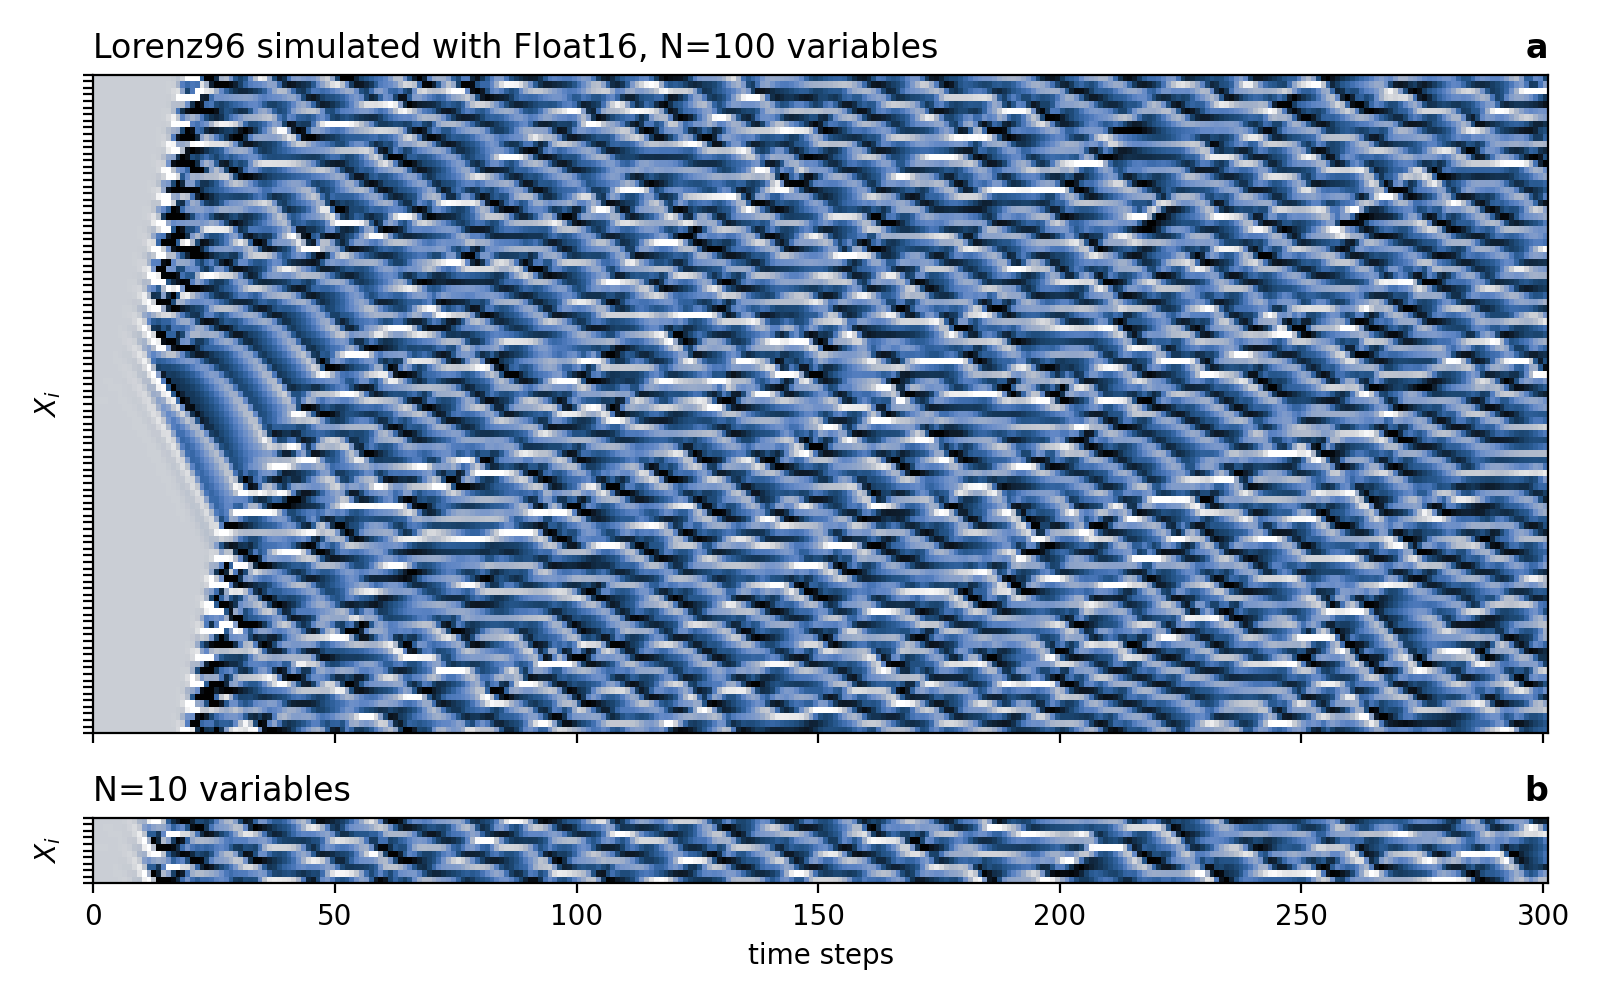
\includegraphics[width=1\textwidth]{Figs/hovmoeller.png}
%\caption{Solution of the Lorenz 1996 model presented as Hovmoeller diagram. (a) Float64 arithmetic, (b) Posit(16,1) arithmetic.}
%\label{fig:L96_hovmoeller}
%\end{figure}

A Hovmoeller diagram illustrates the chaotic dynamics simulated by the Lorenz 1996 model (Fig. \ref{fig:L96_hovmoeller}). The initial perturbation in $X_1$ is advected throughout the domain within the first time steps. After this first wake, the model's state becomes chaotic. Posit(16,1) represents well the dynamic, as shown in the comparison with Float64 for reference.

To quantify the forecast error, we run a set of 1000 forecasts per number format, starting from a random time step of a long control simulation. The simulation with Float64 is taken as reference truth. Float16 has an exponential error growth that starts much earlier than the error growth for Posit(16,1) (Fig. \ref{fig:L96_error}). Both formats have on average an identical error growth rate. Posits clearly cause a reduced rounding error compared to floats at all lead times, making posits a better suited number format for the simulation of the Lorenz 1996 model.

We now use the long control simulation with Float64 to produce a dataset that contains all prognostic variables as well as the arithmetic results of all intermediate terms calculated for the tendencies. 16-bit sonums are trained with this dataset, such that they can self-organize around the numbers that occur most frequently within the Lorenz 1996 model (Fig. \ref{fig:Sonum_decprec}b). Consequently, Sonum16 has a slightly higher decimal precision compared to posits for the mode of the data distribution. A second mode is created for the tendencies, for which numbers of the order of $10^{-1}$ frequently occur. The decimal precision of Sonum16 drastically drops beyond the largest numbers $O(100)$ in the Lorenz 1996 model, as no bitpatterns have to be used to encode these real numbers.

After training, the sonum circle (Fig. \ref{fig:sonum_circle}) is defined. All arithmetic operations are precomputed creating look-up tables for multiplication, addition and subtraction. No look-up table is created for division as the Lorenz 1996 equations (Eq. \ref{eq:L96s}) are written division-free ($s^{-1}$ is precomputed). We can now quantify the forecast error as for floats and posits, running a set of 1000 forecasts from the same initial conditions as used for floats and posits.

Sonum16 has a smaller forecast error compared to posits for the important lead times where the normalised RMSE exceeds 1\% (Fig. \ref{fig:L96_error}). Interestingly, although the error growth is much faster for the first time steps, it levels off afterwards and approaches the same error growth rate as for floats and posits once the normalised RMSE exceeds about 1\%. This points towards a higher potential of Sonum16, when the cause of the initial rapid error growth is understood and circumvented with adjustments in the training method. As discussed in the previous section, sonums can be trained to minimize the average decimal rounding error, an aspect that requires further analysis to understand the optimal distribution of decimal precision for a given application. Nevertheless, sonums already provide perspectives towards an optimal number format for a given application. The main characteristics presumably are: (i) high precision for the most frequently occurring numbers, (ii) a tapered precision towards the smallest numbers and (iii) no redundant bitpatterns for very large and very small numbers that do not occur. Posits fulfill these criteria better than floats, which is likely the reason why they outperform floats in the applications presented here.

%\begin{figure}
%\includegraphics[width=1\textwidth]{Figs/L96_error.pdf}
%\caption{Error growth in the Lorenz 1996 system as simulated with Float16, Posit(16,1) or Sonum16. The error has been normalised by the climatological forecast error. Shaded areas denote the interquartile range of 1000 forecasts with the respective format.}
%\label{fig:L96_error}
%\end{figure}

\subsection{Summary on number formats}
\label{sec:summary_formats}

\begin{table}[htbp]
\center
\begin{tabular}{l | r | r | l | l | r | r}
Format & bits & exp bits & $minpos$ & $maxpos$ & $\epsilon$ &  \% NaR \\
\hline
Float64    & $64$ & $11$ & $5.0 \cdot 10^{-324}$ & $1.8 \cdot 10^{308}$  & $16.3$ & $0.0$ \\
Float32    & $32$ & $8$ & $1.0 \cdot 10^{-45}$ & $3.4 \cdot 10^{38}$ & $7.6$ & $0.4$ \\
Float16    & $16$ & $5$ & $6.0 \cdot 10^{-8}$ & $65504$ & $3.7$ & $3.1$ \\
BFloat16    & $16$ & $8$ & $ 9.2 \cdot 10^{-41}$ & $3.4 \cdot 10^{38}$ & $2.8$ & $0.4$  \\
Float8 & $8$ & $3$ & $1.5 \cdot 10^{-2}$ & $15.5$ & $1.9$ & $12.5$\\
\hline
Posit32    & $32$ & $2$ &  $7.5 \cdot 10^{-37}$ & $7.5 \cdot 10^{37}$ & $8.8$ & $0.0$ \\
Posit(16,1) & $16$ & $1$ & $3.7 \cdot 10^{-9}$ & $3.7 \cdot 10^{9}$ & $4.3$ & $0.0$\\
Posit(16,2) & $16$ & $2$ & $1.4 \cdot 10^{-17}$ & $1.4 \cdot 10^{17}$ & $4.0$ & $0.0$\\
Posit(8,0) & $8$ & $0$ & $1.5 \cdot 10^{-2}$ & $64$ & $2.2$ & $0.4$  \\
\hline
Int16 & $16$ & $0$ & $1$ & $32767$ & $0.8$ & $0$\\
Q6.10 & $16$ & $0$ & $9.8 \cdot 10^{-4}$ & $32.0$ & $3.7$ & $0$\\
\hline
LogFixPoint16 & $16$ & $15$ & $5.4 \cdot 10^{-20}$ & $1.8 \cdot 10^{19}$ & $3.2$ & $0.0$\\
BLogFixPoint16 & $16$ & $15$ & $5.4 \cdot 10^{-20}$ & $9.1 \cdot 10^{18}$ & $2.6$ & $0.0$
\end{tabular}
\vspace{10pt}
\caption{\textbf{Some characteristics of various number formats.} $minpos$ is the smallest representable positive number,
$maxpos$ the largest. The machine precision $\epsilon$, is the decimal precision at $1$ (see section \ref{sec:decimal_precision}).
\% NaR denotes the percentage of bit patterns that represent Not-A-Number (NaN), infinity or Not-A-Real (NaR).}
\label{tab:formats}
\end{table}


\section{Rounding modes}
\label{sec:rounding}

\subsection{Round to nearest}
\label{sec:roundnearest}

\subsection{Stochastic rounding}
\label{sec:stochastic_rounding} 

The default rounding mode for floats and posits is round-to-nearest tie-to-even. In this rounding mode an exact result $x$ is rounded
to the nearest representable number $x_i$. In case $x$ is half-way between two representable numbers, the result will be tied to the
even. A floating-point number $x_i$ is considered to be even, if its significand ends in a zero bit. These special cases are therefore
alternately round up or down, which removes a bias that otherwise persists (see Eq. \ref{eq:biased_rounding} for an example of biased rounding).
Let $x_1$ and $x_2$ be the closest two representable numbers to $x$ and $x_1 \leq x < x_2$ then
\begin{equation}
\op{round}_{\op{nearest}}(x) =
\begin{cases}
x_1 \quad &\op{if} x - x_1 < x_2 - x,  \\
x_1 &\op{if} x-x_1 = x_2 - x \op{~and~} x1 \op{~even}, \\
x_2 &\op{else}.
\end{cases}
\label{eq:roundnearest}
\end{equation}

For stochastic rounding, rounding of $x$ down to a representable number $x_1$ or up to $x_2$ occurs at probabilities that are proportional
to the distance between $x$ and $x_1$, $x_2$, respectively. Let $\delta$ be the distance between $x_1,x_2$, then

\begin{equation}
\op{round}_{\op{stoch}}(x) =
\begin{cases}
x_1 \quad &\op{with~probability}\quad 1 - \delta^{-1}(x - x_1)  \\
x_2 &\op{with~probability}\quad  \delta^{-1}(x - x_1).
\end{cases}
\label{eq:stochround}
\end{equation}

This behaviour is illustrated in Fig. \ref{fig:stochround}. In case that $x$ is already identical with a representable number no rounding is applied
and the chance to obtain another representable number is zero. For $x$ being half way between two representable numbers, the chance of
round up or round down is 50\%. The introduced absolute rounding error for stochastic rounding is always at least as big as for round-to-nearest,
and when low-probability round away from nearest occurs, it can be up to $\pm \delta$, whereas for round-to-nearest the error is bound by
$\pm \tfrac{\delta}{2}$. Although the average absolute rounding error is therefore larger for stochastic rounding, the expected rounding error
decreases towards zero for repeated roundings
\begin{equation}
\lim_{N\to \infty}\frac{1}{N} \sum_i^N \op{round}_{\op{stoch}}(x) = x
\end{equation}
as follows by inserting Eq. \ref{eq:stochround}. Stochastic rounding is therefore exact in expectation.

The stochastic rounding mode is implemented for Float16 and BFloat16. Software emulations of both number formats rely on conversion to Float32,
such that the exact result (to the precision provided by Float32) is known before conversion back to 16 bit. Instead of calculating the probabilities
given in Eq. \ref{eq:stochround}, we add a stochastic perturbation $\xi \in [-\tfrac{\delta}{2},\tfrac{\delta}{2}]$ to $x$ before round-to-nearest.
Let $r$ be uniformly distributed in $[0,1]$ then Eq. \ref{eq:stochround} can then be rewritten as

\begin{equation}
\op{round}_{\op{stoch}}(x) =
\begin{cases}
\op{round}_{\op{nearest}}(x +\tfrac{\delta}{2}(r - \tfrac{x-x_1}{\delta}) \quad & \op{if} x_1 = 2^n \op{~and~} x-x_1 < \tfrac{\delta}{4}  \\
\op{round}_{\op{nearest}}(x + \delta(r-\tfrac{1}{2})) & \op{else}.
\end{cases}
\end{equation}

The special case only occurs for $x$ being within $\tfrac{\delta}{4}$ larger than a floating-point number $x_1 = 2^n$, that means with zero significand.
In this case the distance from $x_1$ to the previous float is only $\tfrac{\delta}{2}$, which has to be accounted for.


\subsection{Efficient bitwise implementations}
\label{sec:bitwiseop}

\section{Error norms}
\label{sec:error_norms}

\subsection{Mean and absolute error}
\label{sec:meanabs_error}

\subsection{Relative error}
\label{sec:relative_error}
	
\subsection{Decimal error and precision}
\label{sec:decimal_precision}

\begin{figure}[tbhp]
	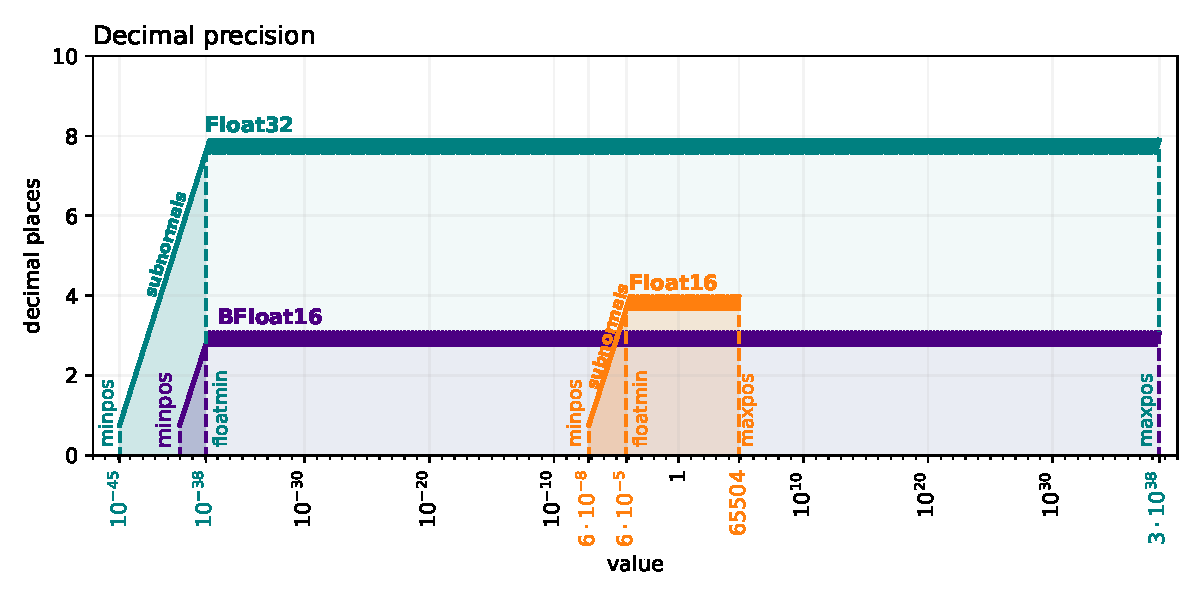
\includegraphics[width=1\textwidth]{Figures/methods/float32_16_bfloat_decprec.pdf}
	\caption{\textbf{Decimal precision of Float16, BFloat16 and Float32 over the range of representable numbers.}
	The decimal precision is worst-case, i.e. given in terms of decimal places that are at least correct after rounding
	(see section \ref{sec:decimal_precision}). The smallest representable number (minpos), the smallest normal number
	(floatmin) and the largest representable number (maxpos) are denoted with vertical dashed lines (see section \ref{sec:floats}).
	The subnormal range is between minpos and floatmin.}
	\label{fig:methods_decprec_floats}
\end{figure}


The decimal precision is defined as \citep{Gustafson2017,Gustafson2017a}
\begin{equation}
\op{decimal} \op{precision} = -\log_{10} \vert \log_{10}( \frac{x_\text{repr}}{x_\text{exact}} ) \vert
\end{equation}
where $x_\text{exact}$ is the exact result of an arithmetic operation and $x_\text{repr}$ is the representable number
that $x_\text{exact}$ is rounded to, given a specified rounding mode. For the common round-to-nearest rounding mode,
the decimal precision approaches infinity when the exact result approaches the representable number and has a minimum
in between two representable numbers. This minimum defines the \emph{worst-case} decimal precision, i.e. the decimal
precision when the rounding error is maximised. The worst-case decimal precision is the number of decimal places that
are at least correct after rounding.

Fig. \ref{fig:decimal_precision} compares the worst-case decimal precision for various 16 and 8-bit floats and posits,
as well as 16-bit integers, the fixed-point format Q6.10 (6 integer bits, 10 fraction bits) and logarithmic fixed-point numbers
LogFixPoint16 and Approx14. Float16 has a nearly constant decimal precision of almost 4 decimal places, which decreases
for the subnormal numbers towards the smallest representable number $minpos$. 16-bit posits, on the other hand, show an
increased decimal precision for numbers around 1 and a wider dynamic range, in exchange for less precision for numbers
around $10^4$ as well as $10^{-4}$.  The machine precision $\epsilon$ (in analogy to the machine error, also known as
machine epsilon), defined as half the distance between 1 and the next representable number, is given in terms of decimal
precision and is summarised in Table \ref{tab:formats} for the various formats. Due to the no overflow/no underflow-rounding
mode, the decimal precision is slightly above zero outside the dynamic range.

The decimal precision of 16-bit integers is negative infinity for any number below 0.5 (round to 0) and maximised for the
largest representable integer $2^{15} - 1 =  32767$. Similar conclusions hold for the fixed-point format Q6.10, as the decimal
precision is shifted towards smaller numbers by a factor of $\tfrac{1}{2}$ for each additional fraction bit.

\section{Type-flexibility through code composability}
\subsection{A type-flexible programming paradigm}

Julia's programming paradigms of \emph{multiple-dispatch} and \emph{type-stability} facilitate the use of arbitrary number formats
without the need to rewrite an algorithm, while compiling functions for specific types \citep{Bezanson2017}. As this is an essential
feature of Julia and extensively made use of here, we briefly outline the benefits of Julia by computing the harmonic sum
$\sum_{i=1}^\infty \tfrac{1}{i}$ with various number types as an example. Analytically the harmonic sum diverges, but with
finite precision arithmetic several issues arise. With an increasing sum the precision is eventually lower than required to
represent the increment of the next summand. The integer i as well as its inverse $\tfrac{1}{i}$ have to be representable
in a given number format, and are also subject to rounding errors.

%\begin{figure}[htbp]
%\small
%\begin{minted}[breaklines,escapeinside=||,mathescape=true,baselinestretch=0.7, linenos, numbersep=3pt, bgcolor=mygray,gobble=2,
%frame=lines, fontsize=\small, framesep=2mm]{julia}
%function harmonic_sum(::Type{T},steps::Int=2000) where T
%
%    s = zero(T)
%    o = one(T)
%
%    for i in 1:steps
%
%        s_old = s
%        s += o/T(i)
%
%        if s == s_old    # check for convergence
%            println(Float64(s),i)
%            break
%        end
%    end
%end
%\end{minted}
%\caption{A type-flexible harmonic sum function in the Julia language.}
%\label{fig:harmsum}
%\end{figure}

Executing the function \texttt{harmonic\_sum} for the first time with a type \texttt{T} as the first argument, triggers Julia's
\emph{just-in-time} compiler (Fig. \ref{fig:harmsum}). The function is type-stable, as the types of all variables are declared
and therefore known to the compiler. At the same time Julia allows for type-flexibility, as its \emph{multiple-dispatch} means
that calling \texttt{harmonic\_sum} with another type \texttt{T2} will result in a separately compiled function for \texttt{T2}.
We can therefore compute the harmonic sum with arbitrary number types, as long as the zero-element \texttt{zero(T)};
the one-element \texttt{one(T)}; addition; division; conversion from integer and conversion to float are defined for \texttt{T}.

%\begin{figure}[htbp]
%\small
%\begin{minted}[breaklines,escapeinside=||,mathescape=true,baselinestretch=0.7, linenos, numbersep=3pt, bgcolor=mygray, gobble=2,
%frame=lines, fontsize=\small, framesep=2mm]{julia}
%julia> using SoftPosit
%julia> using BFloat16s
%julia> harmonic_sum(Float16)
%(7.0859375, 513)
%
%julia> harmonic_sum(BFloat16)
%(5.0625, 65)
%
%julia> harmonic_sum(Posit16)
%(7.77734375, 1024)
%\end{minted}
%\caption{Harmonic sum example use of the posit emulator \emph{SoftPosit.jl} in the Julia shell. \texttt{Posit16} is the Posit(16,1) standard.}
%\label{fig:harmsum2}
%\end{figure}

The harmonic sum converges after 513 elements when using Float16 (Fig. \ref{fig:harmsum2}). The precision of BFloat16
is so low that the sum already converges after 65 elements, as the addition of the next term $1/66$ is rounded back to
5.0625. We identify the addition of small terms to prognostic variables of size $\mathcal{O}(1)$ as one of the major challenges
with low precision arithmetic, which is discussed in more detail in section \ref{sec:mixed}. Using Posit(16,1), the sum only converges
after 1024 terms, due to the higher decimal precision of posits between 1 and 10.

\subsection{Analysis number formats}

\section{Information theory}
\label{sec:information}

\subsection{Entropy}
\label{sec:entropy}

\subsection{Mutual information}
\label{sec:mutual_information}

\subsection{Preserved information}
\label{sec:preserved_information}



\chapter{Information-preserving \nobreak{compression} for climate data}
\label{chap:compression}

%% CONTRIBUTION
\small \paragraph{Contributions} This chapter is largely based on the following publication\footnote{with the following author contributions.
Conceptualisation: MK, MR, JJD. Data curation: MR, JJD, MK. Formal Analysis: MK. Methodology: MK. Visualisation: MK. Writing –
original draft: MK. Writing – review \& editing: MK, PDD, MR, JJD, TNP.}

\vspace{\baselineskip}
\indent M Klöwer, M Razinger, JJ Dominguez, PD Düben and TN Palmer, 2021. \emph{Compressing atmospheric data into its real
information content}, \textbf{Nature Computational Science}, accepted. Preprint \href{https://doi.org/10.21203/rs.3.rs-590601/v1}{10.21203/rs.3.rs-590601/v1}
\vspace{\baselineskip}
\hrule
\vspace{\baselineskip}
\normalsize

\paragraph{Abstract.} Hundreds of petabytes of data are produced annually at weather and climate forecast centres worldwide.
Compression is inevitable to reduce storage and to facilitate data sharing. Current techniques do not distinguish the real from
the false information in data. We define the bitwise real information content from information theory for data from the Copernicus
Atmospheric Monitoring Service (CAMS). Most variables contain less than 7 bits of real information per value, which are also highly
compressible due to spatio-temporal correlation. Rounding bits without real information to zero facilitates lossless compression
algorithms and encodes the uncertainty within the data itself. The entire CAMS data is compressed by a factor of 17x, relative to
64-bit floats, while preserving 99\% of real information. Combined with 4-dimensional compression to exploit the spatio-temporal
correlation, factors beyond 60x are achieved without an increase in forecast errors. A data compression Turing test is proposed to
optimise compressibility while minimising information loss for the end use of weather and climate forecast data. 

\section{Introduction}
\label{sec:compression_introduction}

Many supercomputing centres in the world perform operational weather and climate simulations several times per day \citep{Bauer2015}.
The European Centre for Medium-Range Weather Forecasts (ECMWF) produces 230TB of data on a typical day and
most of the data is stored on magnetic tapes in its archive. The data production is predicted to quadruple within the
next decade due to an increased spatial resolution of the forecast model \citep{Bauer2020,Voosen2020,Schar2020}.
Initiatives towards operational predictions with global storm-resolving simulations, such as Destination Earth
\citep{Bauer2021,Bauer2021a} or DYAMOND \citep{Stevens2019}, with a grid spacing of a couple of
kilometres will further increase data volume. This data describes physical and chemical variables of atmosphere, ocean
and land in up to 6 dimensions: three in space, time, forecast lead time, and the ensemble dimension. The latter results
from calculating an ensemble of forecasts to estimate the uncertainty of predictions \citep{Molteni1996,Palmer2019}.
Most geophysical and geochemical variables are highly correlated in all of those dimensions, a property that is rarely
exploited for climate data compression, although multidimensional compressors are being developed
\citep{Ballester-Ripoll2020,Lindstrom2014,vonLarcher2019,Zhao2020,Di2016}.

Floating-point numbers are the standard to represent real numbers in binary form. 64-bit double precision floating-point
numbers (Float64) consist of a sign bit, 11 exponent bits representing a power of two, and 52 mantissa bits allowing for
16 decimal places of precision across more than 600 orders of magnitude (\cite{IEEE1985} and section \ref{sec:floats}).
Most weather and climate models are based on Float64 arithmetics, which has been questioned as the transition to 32-bit single
precision floats (Float32) does not necessarily decrease the quality of forecasts \citep{Vana2017,TintoPrims2019}. Many bits in Float32
only contain a limited amount of information as even 16-bit arithmetic has been shown to be sufficient for parts of weather
and climate applications \citep{Hatfield2019,Klower2020a,Ackmann2021,Dawson2018,Fan2019}.
The information, as defined by Shannon information theory \citep{Shannon1948,MacKay2003,Kleeman2011},
for simple chaotic dynamical systems is often zero for many of the 32 bits in Float32 \citep{Jeffress2017}.
This supports the general concept of low-precision climate modelling for calculations and data storage, as, at least in theory,
many rounding errors are entirely masked by other uncertainties in the chaotic climate system
\citep{Palmer2014a,Palmer2015}.

The bitwise information content has been formulated for predictability in dynamical systems \citep{Jeffress2017}.
It quantifies how much individual bits in the floating-point representation contribute to the information necessary
to predict the state of a chaotic system at a later point in time. This technique has been used to optimise the
simulation of simple chaotic systems on inexact hardware to reduce the precision as much as possible. Here, we
extend the bitwise information content to distinguish between bits with real and false information in data and to
quantify the preserved real information in data compression. 

Data compression for floating-point numbers often poses a trade-off in size, precision and speed
\citep{Silver2017,Kuhn2016a,Hubbe2013}:
Higher compression factors for smaller file sizes can be achieved with lossy compression, which reduces
the precision and introduces rounding errors. Additionally, higher compression requires more sophisticated
compression algorithms, which can decrease compression and/or decompression speed. A reduction in
precision is not necessarily a loss of real information, as occurring rounding errors are relative to a reference
that itself comes with uncertainty. Here, we calculate the bitwise real information content \citep{Shannon1948,Jeffress2017,Kleeman2011}
of atmospheric data to discard bits that contain no information \citep{Zender2016,Kouznetsov2020} and only compress the real
information content. Combined with modern compression algorithms \citep{Lindstrom2014,Lindstrom2006} the multi-dimensional
correlation of climate data is exploited for higher compression efficiency \citep{Baker2016,Baker2019,Woodring2011}.

\section{Data}
\label{sec:compression_data}

\subsection{Copernicus Atmospheric Monitoring Service}
\label{sec:CAMS}

CAMS data is analysed for one time step on 01/12/2019 12:00 UTC, bilinearly regridded onto a regular 0.4\textdegree{}x0.4\textdegree{}
longitude-latitude grid using climate data operators (cdo) v1.9. All 137 vertical model levels are included.
Furthermore, global fields of temperature from ECMWF’s ensemble prediction system with 91 vertical levels are
used from the first 25 members of a 50-member 15-day ensemble forecast starting on 24 Sept 2020 00:00 UTC.
Bilinear regridding onto a regular 0.2\textdegree{}x0.2\textdegree{} longitude-latitude grid, similar as for the CAMS data, is applied.
All compression methods here include the conversion from Float64 to Float32.

Only longitude-latitude grids are considered in this paper. However, the methodology can be applied to other grids too.
For example, ECMWF’s octahedral grid collapses the two horizontal dimensions into a single horizontal dimension
which circles on latitude bands around the globe starting at the South Pole till reaching the North Pole \citep{Malardel2016}.
Fewer grid points of the octahedral grid reduce the size, but the correlation in latitudinal direction cannot be exploited.

\subsection{Grid definitions}
\label{sec:grid_definitions}

The compression methods described here are applied to gridded binary data. Data on structured grids can be represented as a tensor,
such that for two dimensions that data can be arranged in a matrix $A$  with elements $a_{ij}$ and $i,j$ indices.
Adjacent elements in $A$, e.g. $a_{ij}$ and $a_{i+1,j}$, are also adjacent grid points. Every element $a_{ij}$ is a floating-point number,
or in general a number represented in any binary format. The $n$ bits in $a_{ij}$ are described as bit positions, including sign, exponent
and mantissa bits. In the following we will consider sequences of bits that arise from incrementing the indices $i$ or $j$ while holding the
bit position fixed. For example, the sequence of bits consisting of the first mantissa bit in $a_{ij}$, then the first mantissa bit in $a_{i+1,j}$,
and so on. We may refer to these bits as bits from adjacent grid points. Every bit position in elements of $A$ is itself a matrix, e.g.
the matrix of sign bits across all grid points.

\section{Methods}
\label{sec:compression_methods}

\subsection{Real information content}
\label{sec:real_information}

The Shannon information entropy $H$ in units of bits \citep{Shannon1948} takes for a bitstream $b = b_1b_2...b_k...b_l$, i.e. a sequence
of bits of length $l$, the form
	\begin{equation}
	H = -p_0\log_2(p_0) - p_1\log_2(p_1)
	\label{eq:bit_unconditional_entropy}
	\end{equation}
with $p_0,p_1$ being the probability of a bit $b_k$ in $b$ being $0$ or $1$ (see section \ref{sec:entropy}).
The entropy is maximised to 1 bit for equal probabilities $p_0 = p_1 = \tfrac{1}{2}$ in $b$. We derive the mutual information
\citep{Schreiber2000,Kraskov2004,Pothapakula2019}
of two bitstreams $r = r_1r_2...r_k...r_l$ and $s = s_1s_2...s_k...s_l$ (see section \ref{sec:mutual_information}). The mutual
information is defined via the joint probability mass function $p_{rs}$, which here takes the form of a 2x2 matrix
 	\begin{equation}
	p_{rs} = \begin{pmatrix} p_{00} & p_{01} \\ p_{10} & p_{11} \end{pmatrix}
	\end{equation}
with $p_{ij}$ being the probability that the bits are in the state $r_k = i$ and $s_k = j$ simultaneously and $p_{00} + p_{01} + p_{10} + p_{11} = 1$.
The marginal probabilities follow as column or row-wise additions in $p_{rs}$, e.g. the probability that $r_k = 0$ is $p_{r=0} = p_{00} + p_{01}$.
The mutual information $M(r,s)$ of the two bitstreams $r,s$ is then
	\begin{equation}
	M(r,s) = \sum_{r=0}^1 \sum_{s=0}^1 p_{rs} \log_2 \left( \frac{p_{rs}}{p_{r=r}p_{s=s}} \right)
	\end{equation}
We now consider the two bitstreams $r,s$ being the preceding and succeeding bits (for example in space or time) in a single bitstream $b$,
i.e. $r=b_1b_2...b_{l-1}$ and $s=b_2b_3...b_l$. As explained in section \ref{sec:grid_definitions}, this can for example be the
bitstream of all first mantissa bits in the gridded data. Considering $r,s$ as the preceding and succeeding bits is equivalent to
the bitwise mutual information in adjacent grid points.
The (unconditional) entropy is then effectively $H = H(r) = H(s)$ as in Eq. \ref{eq:bit_unconditional_entropy} and for $l$ being very large.
The conditional entropies $H_0,H_1$ (see section \ref{sec:cond_entropy}) are conditioned on the state of the preceding bit
$b_{k-1}$ being $0$ or $1$, respectively
	\begin{align}
	H_0 &= -p_{00} \log_2(p_{00}) - p_{01} \log_2(p_01)\\
	H_1 &= -p_{10} \log_2(p_{10}) - p_{11} \log_2(p_11) 
	\end{align}
The conditional entropy is maximised to 1 bit for bitstreams where the probability of a bit being 0 or 1 does not depend on the state of the
preceding bit, which is here defined as \emph{false information}. With the conditional and unconditional entropies and $p_0,p_1$ as in
Eq. \ref{eq:bit_unconditional_entropy} the mutual information $M$ of succeeding bits can be written as
	\begin{equation}
	I = H - p_0H_0 - p_1H_1
	\label{eq:realinformation_content}
	\end{equation}
which is the real information content $I$. This definition is similar to \cite{Jeffress2017} but avoids an additional assumption of an uncertainty
measure. Their formulation similarly uses the state of bits as predictors but assesses the conditional probability mass functions of a
dynamical system as predictands. The binwidth of the pdf is chosen to represent the uncertainty in the system, which the bitwise real information
strongly depends on. The formulation here avoids such an additional assumption of uncertainty as bits are used as both predictors and
predictands in the conditional entropy. Consequently, the uncertainty is obtained from the data itself solely based on the mutual information
between bits in adjacent grid points.

Eq. \ref{eq:realinformation_content} defines the real information as the entropy minus the false information. For bitstreams with either $p_0 = 1$
or $p_1=1$, i.e. all bits are either $0$ or $1$, the entropies are zero $H = H_0 = H_1 = 0$ and we may refer to the bits in the bitstream as being unused.
In the case where $H > p_0H_0 + p_1H_1$, the preceding bit is a predictor for the succeeding bit which means that the bitstream contains
real information ($I > 0$).

\subsection{The multidimensional real information content}
\label{sec:multidimensional_real_information}

The real information content $I_m$ for an $m$-dimensional array $A$ is the sum of the real information along the $m$ dimensions.
Let $b_j$ be a bitstream obtained by unravelling a given bitposition in $A$ along its $j$-th dimension. 
Although the unconditional entropy $H$ is unchanged along the $m$-dimensions, the conditional entropies $H_0,H_1$ change as the
preceding and succeeding bit is found in another dimension, e.g. $b_2$ is obtained by reordering $b_1$. $H_0(b_j)$ and $H_1(b_j)$
are the respective conditional entropies calculated from bitstream $b_j$. Normalisation by $\tfrac{1}{m}$  is applied to $I_m$ such
that the maximum information is 1 bit in $I_m^*$
	\begin{equation}
	I_m^* = H - \frac{p_0}{m} \sum_{j=1}^mH_0(b_j) - \frac{p_1}{m}\sum_{j=1}^mH_1(b_j)
	\end{equation}
Due to the presence of periodic boundary conditions for longitude a succeeding bit might be found across the bounds of $A$.
This simplifies the calculation as the bitstreams are obtained from permuting the dimensions of  and subsequent unravelling into a vector.

\subsection{Preserved information}
\label{sec:preserved_information}

We define the preserved information $P(r,s)$ in a bitstream $s$ when approximating $r$ (e.g. after a lossy compression) via the
symmetric normalised mutual information
	\begin{equation}
	R(r,s) = \frac{2M(r,s)}{H(r) + H(s)}
	\end{equation}
$R$ is the redundancy of information of $r$ in $s$. The preserved information $P$ in units of bits is then the redundancy-weighted real information
$I$ in $r$
	\begin{equation}
	P(r,s) = R(r,s)I(r)
	\end{equation}
The information loss $L$ is $1-P$ and represents the unpreserved information of $r$ in $s$. In most cases we are interested in the preserved
information of an array $X = (x_1,x_2,...x_q,...x_n)$ of bitstreams $x$ when approximated by a previously compressed array $Y = (y_1,y_2,...y_q,...y_n)$.
For an array $A$ of floats with $n=~$32 bit, for example, $x_1$ is the bitstream of all sign bits unravelled along a given dimension (e.g. longitudes) and  $x_{32}$
is the bitstream of the last mantissa bits. The redundancy $R(X,Y)$ and the real information $I(X)$ are then calculated for each bit position $q$ individually,
and the fraction of preserved information $P$ is the redundancy-weighted mean of the real information in $X$
	\begin{equation}
	P(X,Y) = \frac{ \sum_{q=1}^n R(x_q,y_q)I(x_q)}{\sum_{q=1}^n I(x_q)}
	\end{equation}
The quantity $\sum_{q=1}^nI(x_q)$ is the total information in $X$ and therefore also in $A$. The redundancy is $R=1$ for bits that are
unchanged during rounding and $R=0$ for bits that are rounded to zero. The preserved information with bitshave or halfshave
\citep{Zender2016,Kouznetsov2020}
(i.e. replacing mantissa bits without real information with either 00...00 or 10...00, respectively) is therefore equivalent to truncating
the bitwise real information for the (half)shaved bits. For round-to-nearest, however, the carry bit depends on the state of bits across 
several bit positions. To account for interdependency of bit positions the mutual information has to be extended to include more bit
positions in the joint probability $p_{rs}$, which will then be a $m \times 2$ matrix. For computational simplicity, we truncate the
real information as the rounding errors of round-to-nearest and halfshave are equivalent.

\subsection{Significance of real information}
\label{sec:significance_real_information}

In the analysis of real information it is important to distinguish between bits with very little but significant information and
those with information that is insignificantly different from zero. While the former have to be retained, the latter should be
discarded to increase compressibility. A significance test for real information is therefore presented.

For an entirely independent and approximately equal occurrence of bits in a bitstream of length $l$, the probabilities $p_0,p_1$
of a bit being $0$ or $1$ approach $p_0 \approx p_1 \approx \tfrac{1}{2}$, but they are in practice not equal for $l<\infty$.
Consequently, the entropy is smaller than 1, but only insignificantly. The probability $p_1$ of successes in the binomial distribution
(with parameter $\tfrac{1}{2}$) with $l$ trials (using the normal approximation for large $l$) is
	\begin{equation}
	p_1 = \frac{1}{2} + \frac{z}{2\sqrt{2}}
	\end{equation}
where $z$ is the $1-\tfrac{1}{2}(1-c)$ quantile at confidence level c of the standard normal distribution. For $c = 0.99$ corresponding
to a 99\%-confidence level which is used as default here, $z = 2.58$ and for $l = 5.5 \cdot 10^7$  (the size of a 3D array from CAMS)
a probability $\tfrac{1}{2} \leq p \leq p_1 = 0.5002$ is considered insignificantly different from equal occurrence $p_0 = p_1$.
The associated free entropy $H_f$ in units of bits follows as
	\begin{equation}
	H_f = 1 - p_1\log_2(p_1) - (1-p_1)\log_2(1-p_1)
	\end{equation}
We consider real information below $H_f$ as insignificantly different from 0 and set the real information $I = 0$.

\begin{figure}[tbhp]
	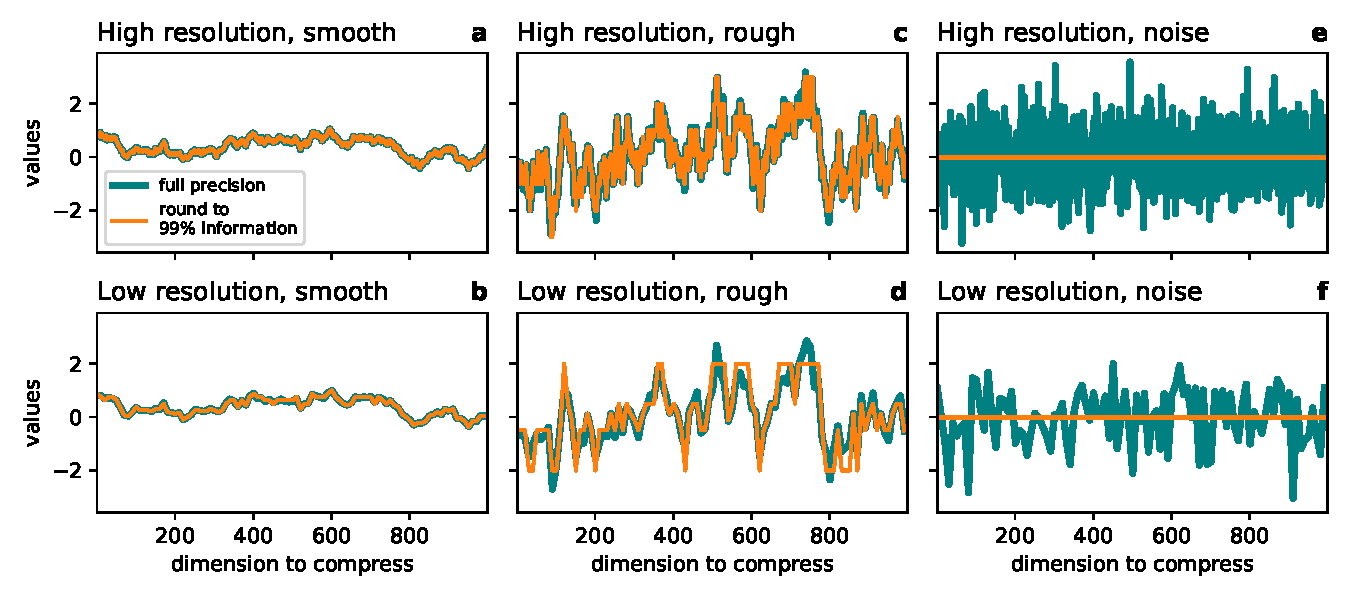
\includegraphics[width=1\textwidth]{Figures/compression/resolution_information.pdf}
	\caption{\textbf{Resolution and smoothness dependence of the information-preserving compression. a,b}
	Highly autocorrelated data (1st order auto-regressive process with correlation $r=0.999$) will have many
	mantissa bits preserved, at high and low resolution. \textbf{c,d} Many mantissa bits in data with less autocorrelation
	($r=0.95$) will be independent at low resolution and therefore rounded to zero. \textbf{e,f} All bits in random data ($r=0$)
	drawn from a standard normal distribution are fully independent so that removing the false information rounds
	this data to zero. Low resolution data (\textbf{b,d,f}) is obtained from high resolution (\textbf{a,c,e}) by subsampling every
	10th data point.}
	\label{fig:information_resolution}
\end{figure}

\subsection{Dependency of the bitwise real information on correlation}
\label{sec:information_correlation}

The real information as defined here depends on the mutual information of bits in adjacent grid points.
Higher autocorrelation in data (meaning a higher correlation between adjacent grid points) increases the
mutual information in the mantissa bits. With higher correlation the adjacent grid values are closer,
increasing the statistical dependence of mantissa bits that would otherwise be independent at lower correlation.
Consequently, the real bitwise information content is increased and more mantissa bits have to be retained to
preserve 99\% of real information (Fig. \ref{fig:information_correlation}a and b).

The increasing number of retained mantissa bits with higher autocorrelation in data will decrease compression factors,
as it is easier to compress bits that are rounded to zero. However, a higher correlation also increases the redundancy
in bits of adjacent grid points, which favours a more efficient lossless compression. These two effects counteract and
compression factors only increase piecewise over a small range of correlations while the retained mantissa bits are
constant (Fig. \ref{fig:information_correlation}c and d). Once an additional mantissa bit has to be retained to preserve
99\% of real information, compression factors jump back down again, resulting in a sawtooth wave. Over a wide
range of typical correlation coefficients (0.5 - 0.9999) the compression factors are otherwise constant and no higher
compressibility is found with increased correlation. 

\begin{figure}[tbhp]
	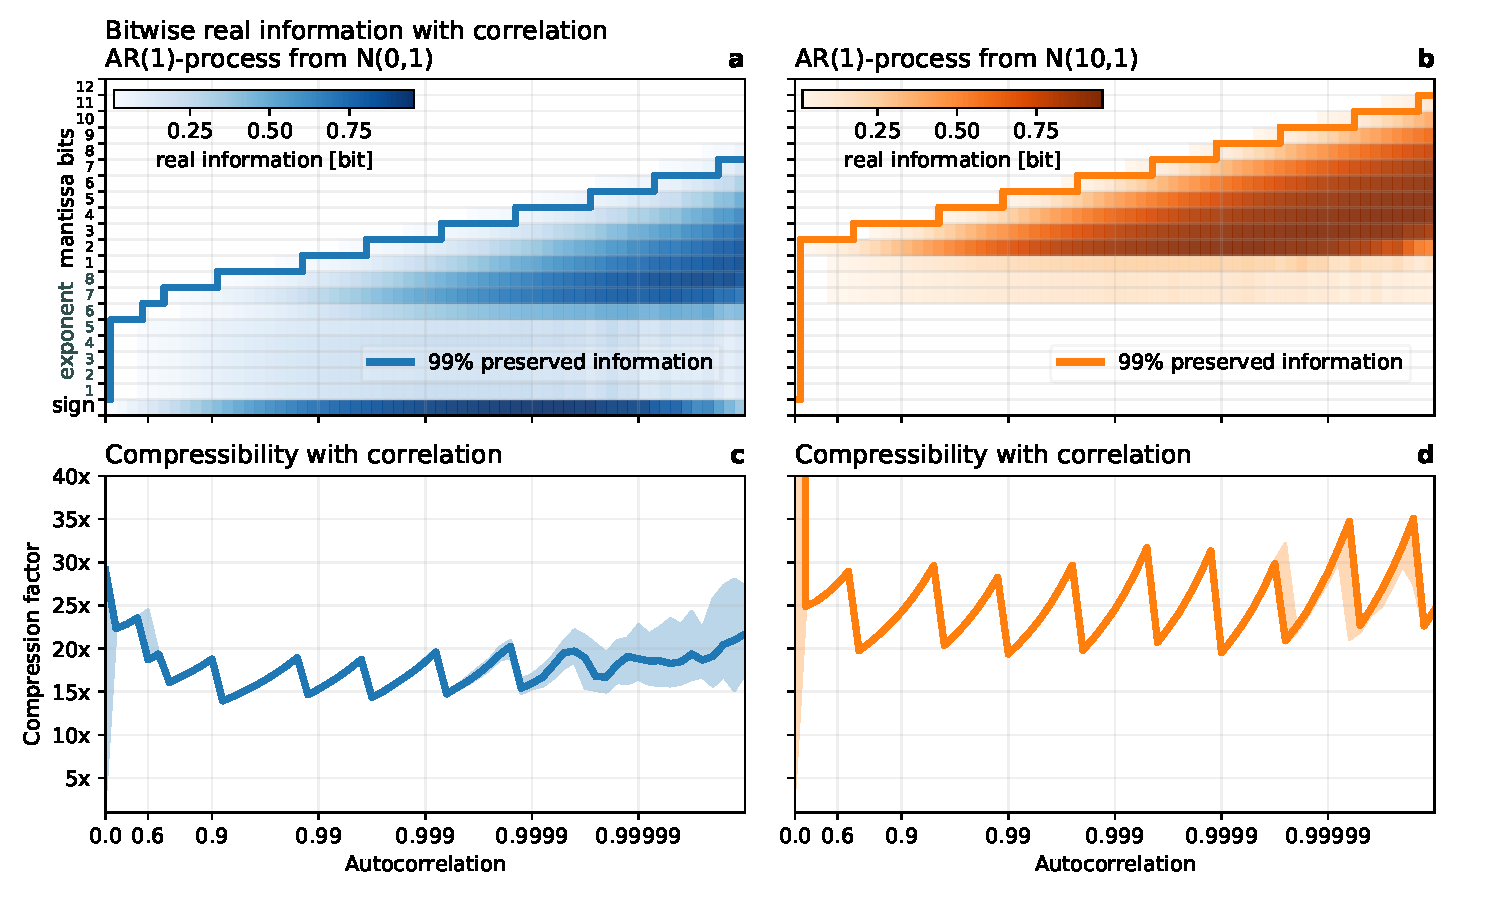
\includegraphics[width=1\textwidth]{Figures/compression/correlation_ar1.pdf}
	\caption{\textbf{Dependency of the bitwise real information and compressibility on correlation. a}
	The bitwise real information content of a first-order autoregressive process (AR(1) with Gaussian distribution N(0,1),
	i.e. with zero mean and unit variance) with varying lag-1 autocorrelation. The bits that have to be retained to preserve
	99\% of information are enclosed with a solid line. \text{b} as \textbf{a} but the AR(1) process follows a Gaussian distribution with
	a mean of 10. \textbf{c,d} Compression factors for \textbf{a,b} when preserving 99\% of information. Shading denotes the interdecile range.}
	\label{fig:information_correlation}
\end{figure}

The compression factors can, however, depend on the range of values represented in binary: A shift in the mean to have
positive or negative values only means that the sign bit is unused, which increases compression factors
(compare Fig. \ref{fig:information_correlation}a with b), despite identical correlation coefficients. Although the correlation
is invariant under multiplicative scaling and addition, the bitwise information changes under addition: When the range of
values in data fits into a power of two its real information is shifted across bit positions into the mantissa bits, such that
the exponent bits are unused. This can be observed for atmospheric temperatures stored in Kelvin (within 200-330K)
where only the last exponent bit and mantissa bits contain information (Fig. \ref{fig:ensemble_information}).
Using Celsius instead shifts information from the mantissa bits into the exponent and sign bits.

\subsection{Limitations of the information-preserving compression}
\label{sec:information_limitation}

The definition of real information presented here is based on the mutual information in adjacent grid points.
We therefore assume a spatial and temporal coherence of data that will come with some autocorrelation.
For vanishing autocorrelation in the data the real information content will drop to zero, as the mutual information
between bits in adjacent but independent grid points approaches zero. In this case the entire dataset is identified
as false information and consequently rounded to zero. In practice, this only occurs with data having autocorrelation
coefficients of less than 0.2 (Fig. \ref{fig:information_correlation}). If there is valuable scientific information in such
seemingly random data, then the underlying assumption that real information is identified by the mutual information
in adjacent grid points does not hold. 

Issues with the bitwise real information content can arise in data that was previously subject to lossy compression:
Linear or logarithmic quantization, for example, rounds data in linear or logarithmic space, respectively, which is not
equivalent to binary rounding in the floating-point format. Consequently, such a quantization will generally introduce
non-zero bits in the mantissa of floats when decompressed. These bits can have some statistical dependence,
appearing as artificial information induced by the quantization. Such artificial information can be observed as a
small background information (i.e. the bitwise real information is always significantly different from 0) or a reemerging
information in the last mantissa bits. In this case, the information distribution across bit positions deviates clearly from
the typical, where the information drops monotonically in the mantissa bits and becomes insignificantly different from
0 (see the examples in Fig. \ref{fig:bitinformation}, \ref{fig:information_correlation}, \ref{fig:information_error_ssim} or
\ref{fig:ensemble_information}). A solution to this quantization-induced artificial information is to apply the bitwise real
information analysis not on the decompressed floats but on the rounded integers representing the compressed data
in linear or logarithmic quantization. The bitwise real information content as defined here is independent of the binary
format and therefore can be applied to floats as well as the unsigned integers from quantization. Note that this issue
does not arise when rounding is applied in the same encoding which is also used to analyse the real information content.
In our case, using the floating-point representation for the rounding (i.e. removing the false information) the rounded
mantissa bits are always 0 which also means zero entropy when analysing the information. Applying the rounding for
floats repeatedly will have no effect beyond the first application (idempotence).

\begin{figure}[tbhp]
	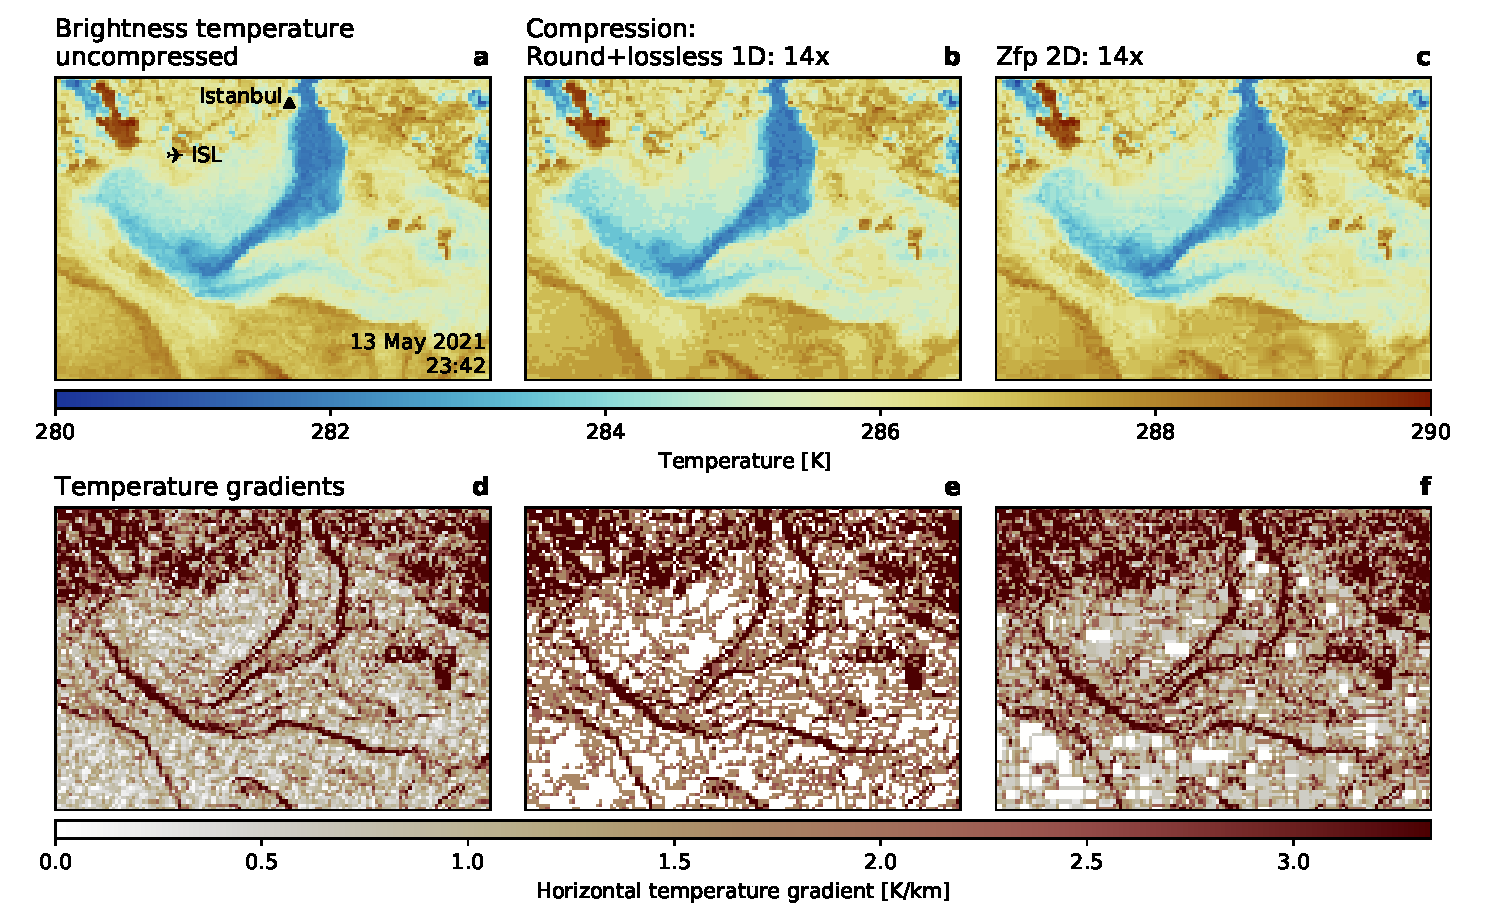
\includegraphics[width=1\textwidth]{Figures/compression/brightness_temp_grad.pdf}
	\caption{\textbf{Preservation of gradients during compression.} Compressing the brightness temperature
	of Fig. \ref{fig:brightness_temp} (VIIRS sensor aboard the satellite Suomi NPP) south of Istanbul where
	the Black Sea outflows into the Marmara Sea. Oceanic fronts with strong horizontal gradients in sea surface
	temperature are visible. \textbf{a} Brightness temperature uncompressed. \textbf{b} as \textbf{a} but compressed
	using round+lossless preserving 99\% of real information. \textbf{c} as \textbf{a} but using Zfp compression in the
	two horizontal dimensions. \textbf{d} Horizontal temperature gradient uncompressed highlighting the oceanic
	fronts from \textbf{a}. \textbf{e} as \textbf{a} but the horizontal gradient is calculated from the round+lossless
	compressed dataset as shown in \textbf{b}. \textbf{f} as \textbf{e} but using Zfp compression as shown in \textbf{c}. 
	The coarseness of the visualisation represents the resolution of the data.
	Istanbul (Hagia Sophia) and Atatürk Airport (ISL) are marked for orientation.}
	\label{fig:compression_gradients}
\end{figure}

\subsection{Preservation of gradients}
\label{sec:preservation_gradients}

The preservation of gradients and other higher-order derivatives in data is a challenging aspect of compression.
Removing false information in data via rounding can result in identical values in adjacent grid points. Even if these values
were not identical before rounding, they may not be significantly different from each other in the sense of real and false
information. In this case, a previously weak but non-zero gradient will be rounded to zero. In other cases the rounding error
is small compared to the standard deviation of the data, such that rounding has a negligible impact on the variance as
values are independently equally likely to be round up or down.

This can be illustrated in the example of analysing oceanic fronts obtained from satellite measurements of sea surface
temperatures (Fig. \ref{fig:compression_gradients}). Identified by large horizontal gradients in temperature, the location
and strength of oceanic fronts is well preserved using compressed data. However, areas of very weak gradients can
largely vanish with round+lossless (Fig.  \ref{fig:compression_gradients}e). In this case the temperature in adjacent grid
points is insignificantly different from each other and therefore the gradient zero after the removal of false information.
Weak gradients are better preserved with Zfp compression at similar compression factors, but its block structure becomes
visible (Fig. \ref{fig:compression_gradients}f). 

\subsection{Structural similarity}
\label{sec:structural_similarity}

A metric to assess the quality of lossy compression in image processing is the structural similarity index measure (SSIM, \cite{Wang2004}).
For images it is based on comparisons of luminance, contrast and structure. For floating-point arrays the luminance contributions
to SSIM can be interpreted as the preservation of the mean; the contrast compares the variances and the structure compares the
correlation. The SSIM of two arrays $A,B$ of same size is defined as
	\begin{equation}
	\op{SSIM}(A,B) = \frac{(2\mu_A\mu_B + c_1)(2\sigma_{AB} + c_2)}{(\mu_A^2 + \mu_B^2 + c_1)(\sigma^2_A + \sigma^2_B + c_2)}
	\end{equation}
With $\mu_A,\mu_B$ the respective means, $\sigma^2_A,\sigma^2_B$ the respective variances and $\sigma_{AB}$ the covariance.
$c_1 = (k_1L)^2$ and $c_2 = (k_2L)^2$  are introduced to increase stability with a small denominator and $k_1 = 0.01, k_2 = 0.03$.
The dynamic range is $L = \max(\max(A),\max(B)) - \min(\min(A),\min(B))$. The SSIM is a value in $[0,1]$ where the best possible
similarity $\op{SSIM}=1$ is only achieved for identical arrays.

\begin{figure}[tbhp]
	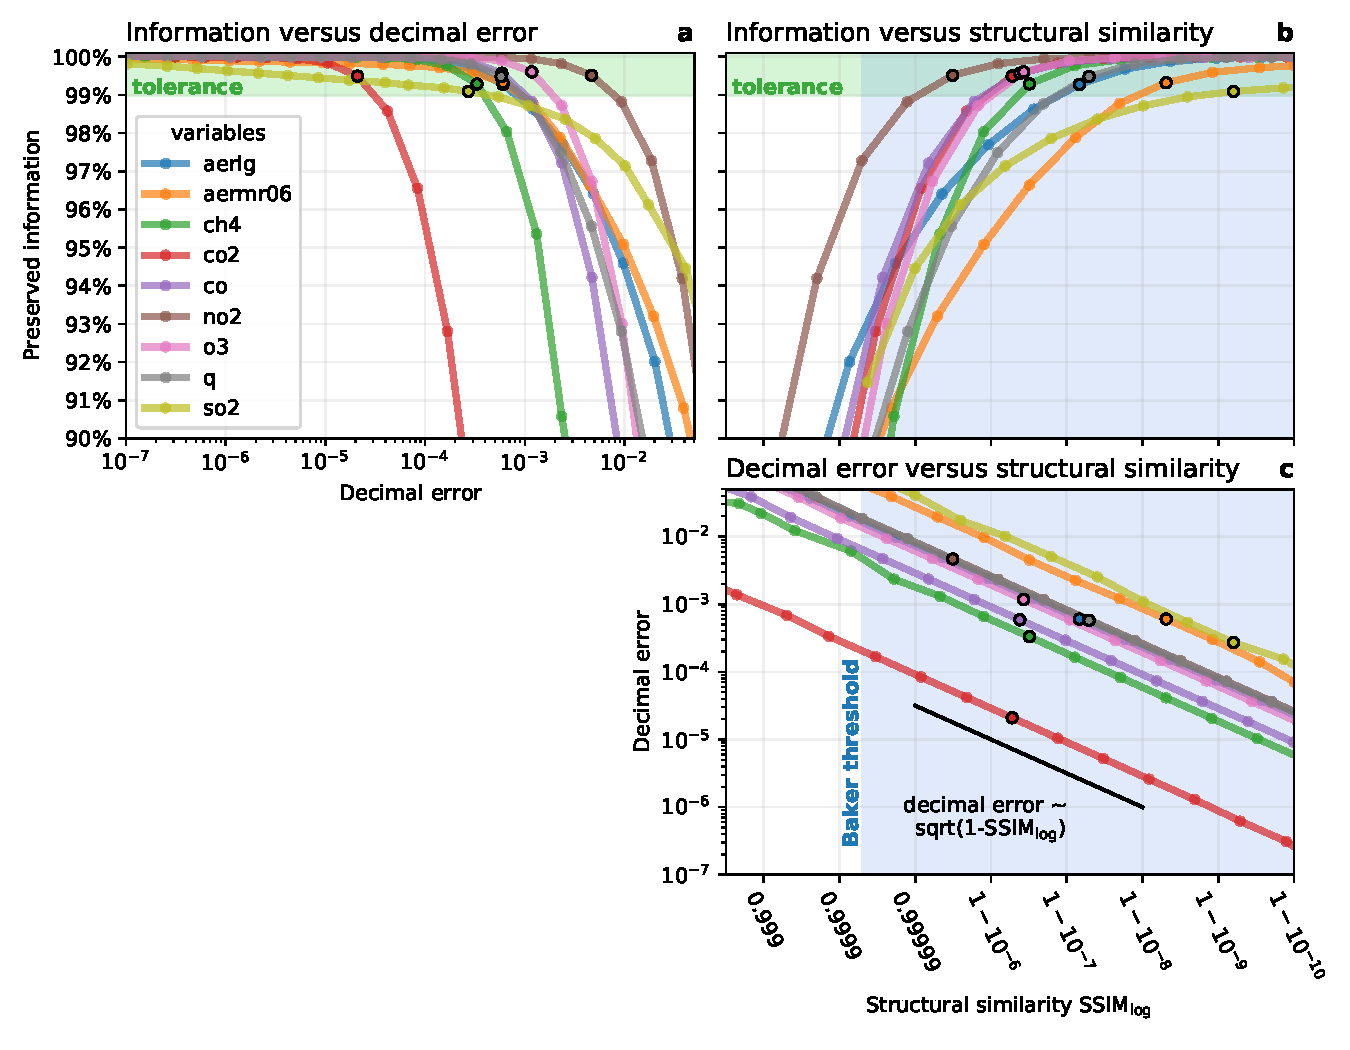
\includegraphics[width=1\textwidth]{Figures/compression/information_error_ssim.pdf}
	\caption{\textbf{The relationships between preserved information, decimal error and structural similarity for rounding within
	the information-preserving compression. a} The last 1\% of information tends to be distributed across many mantissa bits
	such that a trade-off arises where a large increase in compressibility is achieved for a small tolerance in information loss.
	The preserved information is presented as a function of the decimal error, which itself increases exponentially for
	every additional bit (small circles) that is discarded due to rounding. Denoted circles present the number of mantissa bits
	that have to be retained during compression to preserve at least 99\% of information. \textbf{b} The preserved information
	increases as a function of the structural similarity (SSIM, \cite{Wang2004}). The proposed threshold for climate data of
	SSIM=0.99995 by \cite{Baker2019} is shaded. All variables are very close or above the Baker threshold when preserving
	99\% of information. \textbf{c} The decimal error is proportional to the square root of the structural dissimilarity 1-SSIM
	for binary rounding within the information-preserving compression}
	\label{fig:information_error_ssim}
\end{figure}

For rounded floating-point arrays the decimal error is proportional to the square root of the dissimilarity $1-\op{SSIM}$
(Fig. \ref{fig:information_error_ssim}c). The SSIM in this case is approximately equal to the correlation, as round-to-nearest is
bias-free (i.e. $\mu_A \approx \mu_B$) and as the rounding error is typically much smaller than the standard deviation of the data
(i.e. $\sigma_A \approx \sigma_B$). Here, we use the logarithmic SSIM, $\op{SSIM}_{\log}(A,B) = \op{SSIM}(\log(A),\log(B))$,
which is the SSIM applied to log-preprocessed data (the logarithm is applied element-wise). The usage of SSIM$_{\log}$
is motivated due to the rather logarithmic data distribution for most variables (Fig. \ref{fig:cams_histograms}),
but similar results are obtained for SSIM. The proportionality to the decimal error is unchanged when using SSIM$_{\log}$.

\cite{Baker2019} propose the SSIM as a quality metric for lossy compression of climate data52. While for image processing
SSIM > 0.98 is considered good quality, \cite{Baker2019} suggest a higher threshold of SSIM = 0.99995 for climate data compression.
The preserved information as defined here can be used as a compression quality metric similar to the SSIM. When preserving 99\%
of real information the SSIM$_{\log}$ is also above the Baker threshold (Fig. \ref{fig:information_error_ssim}b), reassuring that our
threshold of 99\% preserved real information is reasonable. In general, the preserved information is a monotonic function of the
structural similarity SSIM (or SSIM$_{\log}$) for rounded floating-point arrays, further supporting the usage of preserved
information as a metric for data compression. 

\subsection{Linear and logarithmic quantization}
\label{sec:linlogquantization}

The $n$-bit linear quantization compression for each element $a$ in an array $A$ is
	\begin{equation}
	\tilde{a} = \op{round} \left( 2^{n-1} \frac{a - \min(A)}{\max(A) - \min(A)} \right)
	\end{equation}
with $\op{round}$ a function that rounds to the nearest integer in $0,...,2^{n-1}$. Consequently, every compressed element $\tilde{a}$
can be stored with $n$ bits. The $n$-bit logarithmic quantization compression for every element $a\geq0$ in $A$ is
	\begin{equation}
	\tilde{a} = \begin{cases} 0 \quad &\text{if } a = 0, \\
	\text{round}\left( c + \Delta^{-1}\log(a) \right) + 1 \quad &\text{else.} \end{cases}
	\end{equation}
which reserves the bit pattern zero to encode 0. The logarithmic spacing is
	\begin{equation}
	\Delta = \frac{\log(\max(A)) - \log(\min^+(A))}{2^{n}-2}
	\end{equation}
The constant $c = 1/2 - \Delta^{-1}\log(\text{min}^+(A)(\exp(\Delta)+1)/2)$ is chosen to implement round-to-nearest in linear space
instead of in logarithmic space, for which $c=-\Delta^{-1}\log(\text{min}^+(A))$. The function $\min^+(A)$  is the minimum of all
positive elements in $A$. For a more general discussion on round-to-nearest for logarithmic numbers formats see section
\ref{sec:roundnearest_logfix}.

\subsection{Lossless compression}
\label{sec:compression_lossless}

We use Zstandard as a default lossless algorithm for the round+lossless method. Zstandard is a modern compression algorithm
that combines many techniques to form a single compressor with tunable 22 compression levels that allow large trade-offs between
compression speed and factors \citep{Skibinski2020,Collet2020}. Here, we use compression level 10, as it presents a reasonable
compromise between speed and size. Zstandard outperforms other tested algorithms (deflate, LZ4, LZ4HC and Blosc) in our
applications and is also found to be among the best in the lzbench compression benchmark \citep{Skibinski2020} and other studies
have focused on comparisons \citep{Delaunay2019}. Lossless compressors
are often combined with reversible transformations that preprocess the data. The so-called bitshuffle transposes an array on the
bit-level, such that bit positions (e.g. the sign bit) of floating-point numbers are stored next to each other in memory. Another example
is the bitwise XOR-operation \citep{Pelkonen2015} with the preceding floating-point value, which sets subsequent bits that are identical
to 0. Neither bitshuffle nor XOR significantly increased the compression factors in our applications.

\begin{figure}[tbhp]
	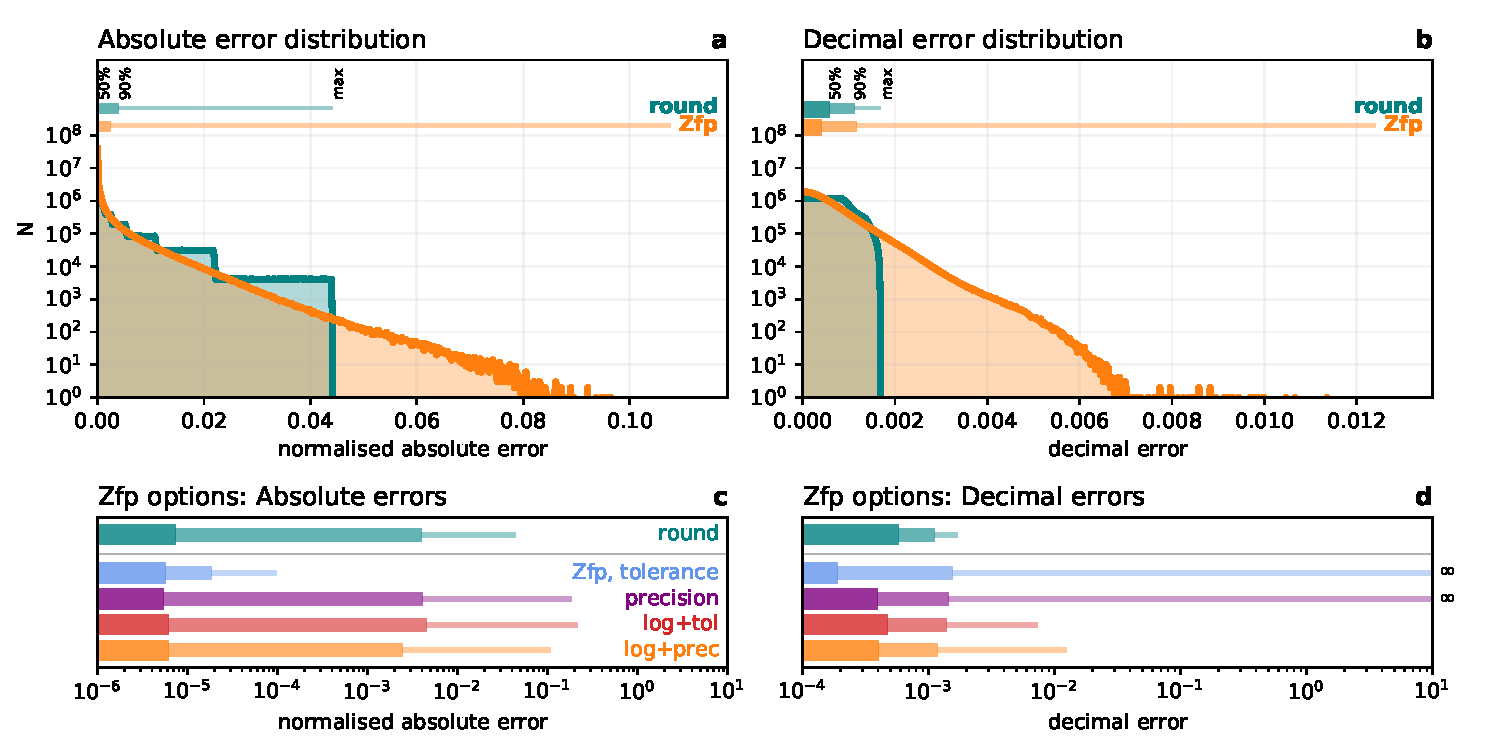
\includegraphics[width=1\textwidth]{Figures/compression/error_distributions.pdf}
	\caption{\textbf{Error distribution of binary rounding compared to Zfp compression.} 
	IEEE round-to-nearest and Zfp compression of water vapour (specific humidity) in the
	three spatial dimensions. \textbf{a, c} normalised absolute errors \textbf{b, d} decimal errors.
	7 mantissa bits are retained for rounding corresponding to 99\% preserved information.
	The precision parameter of Zfp is chosen to yield median errors that are at least as small
	as those obtained by rounding. \textbf{c, d} Zfp via specifying tolerance (tol) or precision (prec)
	with and without log-preprocessing. Maximum decimal errors that reached infinity in \textbf{d}
	due to sign changes are marked.}
	\label{fig:compression_error_distribution}
\end{figure}

\subsection{Matching retained bits to Zfp's precision}
\label{sec:zfp_compression}

The Zfp compression algorithm divides a $d$-dimensional array into blocks of size $4^d$ to exploit correlation
in every dimension of the data. Within each block a transformation of the data is applied with specified absolute
error tolerance or precision, which bounds a local relative error. We use Zfp in its precision mode, which offers
discrete levels to manually adjust the retained precision. Due to the rather logarithmic distribution of CAMS data
(Fig. \ref{fig:cams_histograms}), a log-preprocessing of the data is applied to prevent sign changes (including a flushing to zero) within
the compression. The error introduced by Zfp is approximately normally distributed and therefore usually yields
higher maximum errors compared to round-to-nearest in float arithmetic, although median errors are comparable.
In order to find an equivalent error level between the two methods, we therefore choose the precision level of Zfp
to yield median absolute and decimal errors that are at least as small as those from rounding.

This method is illustrated in Fig. \ref{fig:compression_error_distribution} in more detail: Errors introduced from
round-to-nearest for floats have very rigid error bounds, the majority of errors from Zfp compression are within
these bounds when matching median errors. However, given the normal distribution of errors with Zfp, there will
be a small share of errors that is beyond the bounds from round-to-nearest. Using the precision mode of Zfp and
log-preprocessed data bounds these maximum errors well (Fig. \ref{fig:compression_error_distribution}c and d).

\begin{figure}[tbhp]
	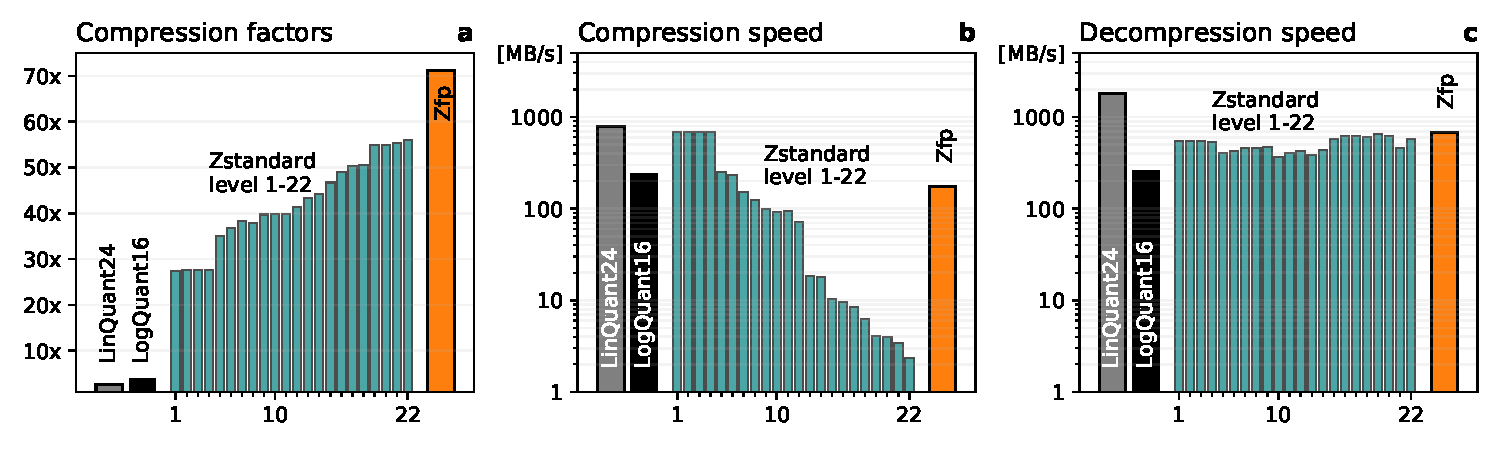
\includegraphics[width=1\textwidth]{Figures/compression/compression_speed.pdf}
	\caption{\textbf{Compressor performances.} 
	Compressing water vapour (specific humidity, variable code q) (3 mantissa bits retained, as in Fig.
	\ref{fig:map_roundlossless_zfp}) with 24-bit linear quantization (LinQuant24), 16-bit logarithmic quantization
	(LogQuant16), round+lossless (Zstandard, compression level 1-22) and Zfp (precision-mode,
	including log-preprocessing): \textbf{a} Compression factors, \textbf{b} compression speed, \textbf{c}
	decompression speed. Timings are single-threaded on an Intel Core\texttrademark~i7 (Kaby Lake) and do not include the writing to disk.}
	\label{fig:compression_speed}
\end{figure}

\subsection{Compressor performances}
\label{sec:compressor_performance}

Although different compressors and their performance are not within the central focus of this chapter, we analyse
the compression and decompression speeds as a sanity check (Fig. \ref{fig:compression_speed}). In order to
find a data compression method that can be used operationally, a certain minimum data throughput should be achieved.
The current 24-bit linear quantization method reaches compression speeds of almost 800 MB/s single-threaded on an
Intel Core\texttrademark~i7 (Kaby Lake) CPU in our application, excluding writing to disk. For the logarithmic quantization,
this decreases to about 200 MB/s due to the additional evaluation of a logarithm for every value. For Zstandard the user
can choose between 22 compression levels, providing a trade-off between the compression speed (highest for level 1)
and the compression factor (highest for level 22). Compression speed reduces from about 700 MB/s at compression level 1
to 2 MB/s at level 22 (Fig. \ref{fig:compression_speed}b), such that for high compression factors about a thousand cores
would be required in parallel to compress in real time the 2GB/s data production at ECMWF. For Zstandard at compression
level 10 speeds of at least 100MB/s are achieved, but at the cost of about 50\% larger file sizes. We use compression level
10 throughout this chapter as a compromise. The decompression speed is independent of the level (Fig. \ref{fig:compression_speed}c).
The additional performance cost of binary rounding is with 2 GB/s negligible. Zfp reaches compression speeds of about 200 MB/s
(single-threaded, including the log-preprocessing) in our application, enough to compress ECMWF’s data production in real
time with a small number of processors in parallel.

\begin{figure}[tbhp]
	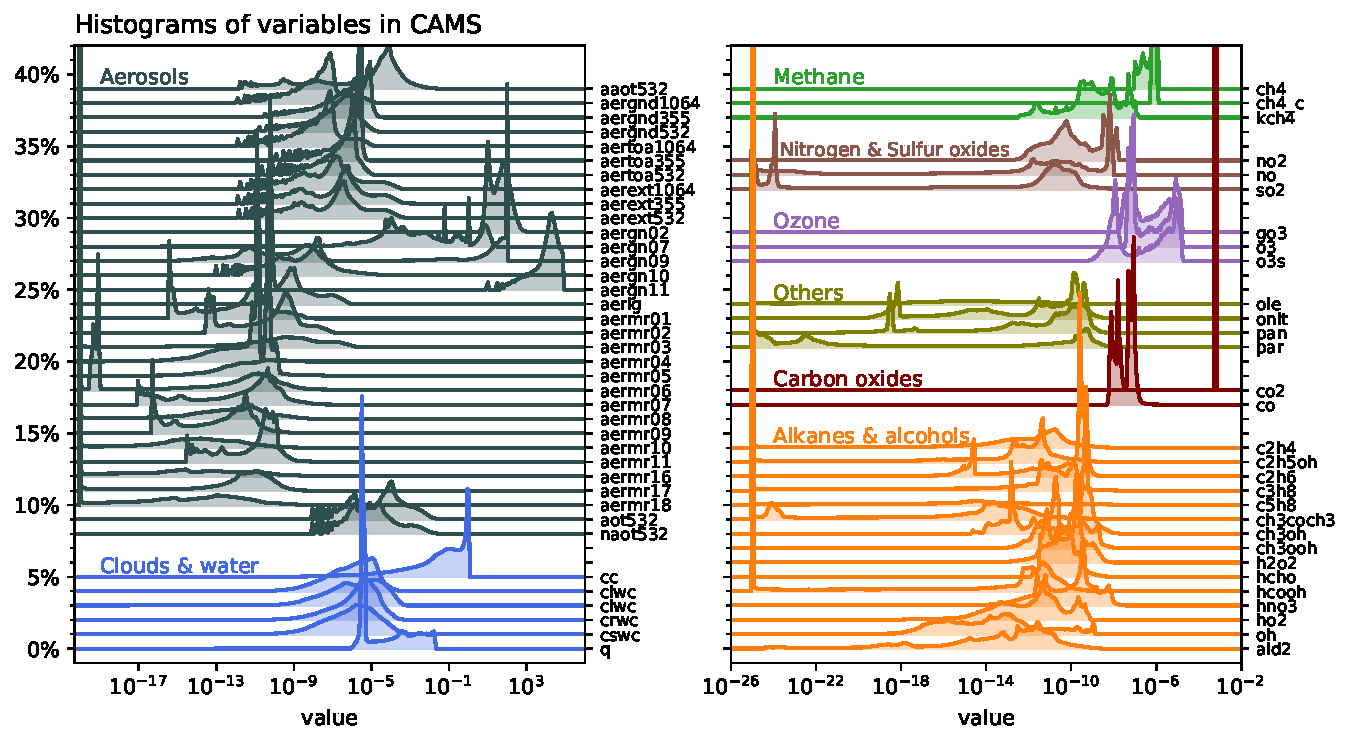
\includegraphics[width=1\textwidth]{Figures/compression/histograms.pdf}
	\caption{\textbf{Statistical distributions of all variables in CAMS.}
	Histograms use a logarithmic binning and are staggered vertically for clarity.
	The variable abbreviations are explained in Table \ref{tab:cams_abbreviations}.}
	\label{fig:cams_histograms}
\end{figure}

\section{Results}
\label{sec:compression_results}
\subsection{Drawbacks of current compression methods}

The Copernicus Atmospheric Monitoring Service (CAMS, \cite{Inness2019}) is performing operational predictions with an extended
version of the Integrated Forecasting System IFS, the global atmospheric forecast model implemented by ECMWF.
CAMS includes various atmospheric composition variables, like aerosols, trace and greenhouse gases that are
important to monitor global air quality. The system monitors for example the spread of volcanic eruptions or
emissions from wildfires. Most variables in CAMS have a multi-modal statistical distribution, spanning many
orders of magnitude (Fig. \ref{fig:cams_histograms}).

The current compression technique for CAMS is the linear quantization, widely used in the weather and climate
community through the data format GRIB2 \citep{WMO2003}. CAMS uses the 24-bit version, which encodes values
in a data array with integers from $0$ to $2^{24}-1$ (see section \ref{sec:linlogquantization}). These 24-bit unsigned
integers represent values linearly distributed in the min-max range. Unused sign or exponent bits from the floating-point
representation are therefore avoided and some of the trailing mantissa bits are discarded in quantization. Choosing the
number of bits for quantization determines the file size, but the precision follows implicitly, leaving the required precision
or amount of preserved information unassessed.

\begin{figure}[tbhp]
	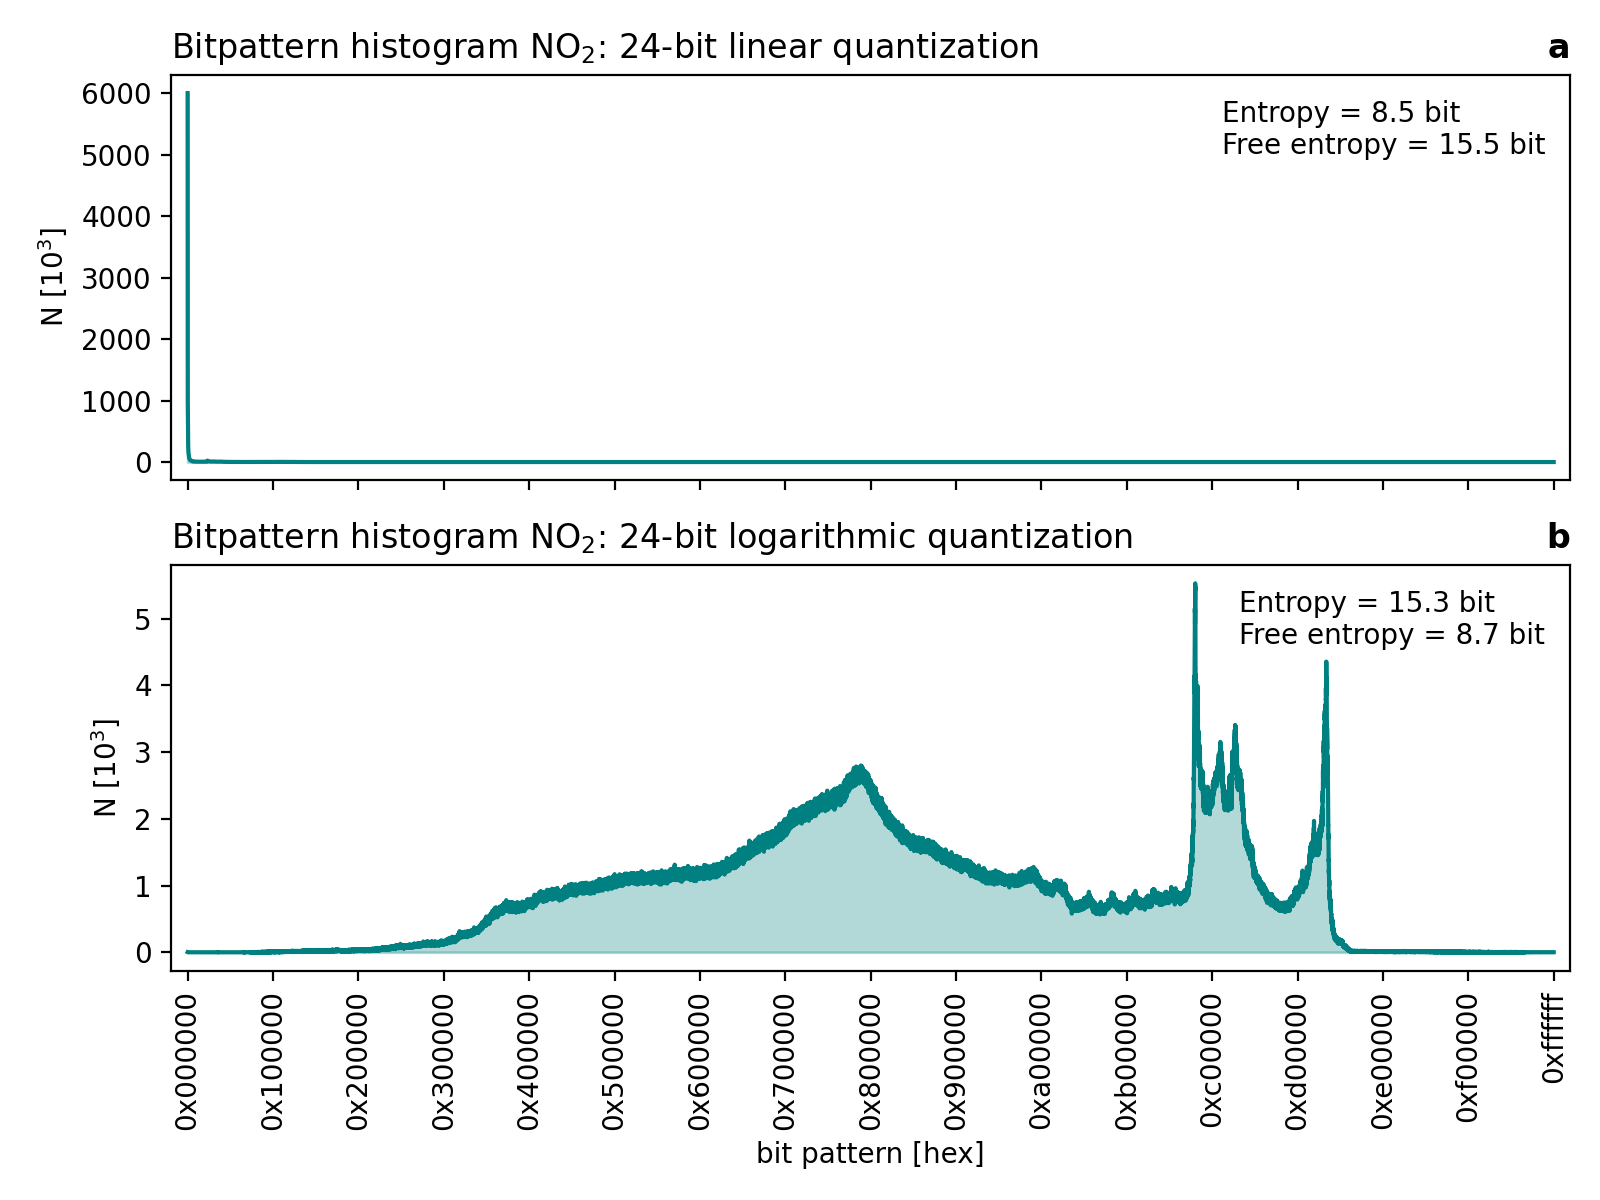
\includegraphics[width=1\textwidth]{Figures/compression/bitpattern_hist.png}
	\caption{\textbf{Bitpattern histogram for linear and logarithmic quantization. a}
	Linear 24-bit quantization and \textbf{b} 24-bit logarithmic quantization of nitrogen dioxide NO\textsubscript{2} mixing ratio [kg/kg].
	All grid points and all vertical levels are used, consisting of $5.6 \cdot 10^7$ values with a range of $2 \cdot 10^{-14}$ to
	$2 \cdot 10^{-7}$ kg/kg. Bitpatterns are denoted in 24-bit hexadecimal. The free entropy is the difference between the
	available 24 bit and the bitpattern entropy and quantifies the number of effectively unused bits.}
	\label{fig:compression_bitpattern_hist}
\end{figure}

Although linear quantization bounds the absolute error, its linear distribution is unsuited for most variables in CAMS:
Many of the available 24 bits are effectively unused as the distribution of the data and the quantized values match
poorly (Fig. \ref{fig:compression_bitpattern_hist}). Alternatively, placing the quantized values logarithmically in the
min-max range better resolves the data distribution. As floating-point numbers are already approximately logarithmically
distributed, this motivates compression directly within the floating-point format, which is also used for calculations in a
weather or climate model and post-processing.

\subsection{Bitwise real information content}

Many of the trailing mantissa bits in floating-point numbers occur independently and at similar probability,
i.e. with high information entropy \citep{Kleeman2011,Jeffress2017}. These seemingly random bits are
incompressible \citep{MacKay2003,Ziv1977,Huffman1952}, reducing
the efficiency of compression algorithms. However, they probably also contain a vanishing amount of real
information, which has to be analysed to identify bits with and without real information. The former should
be conserved while the latter should be discarded to increase compression efficiency.

\begin{figure}[tbhp]
	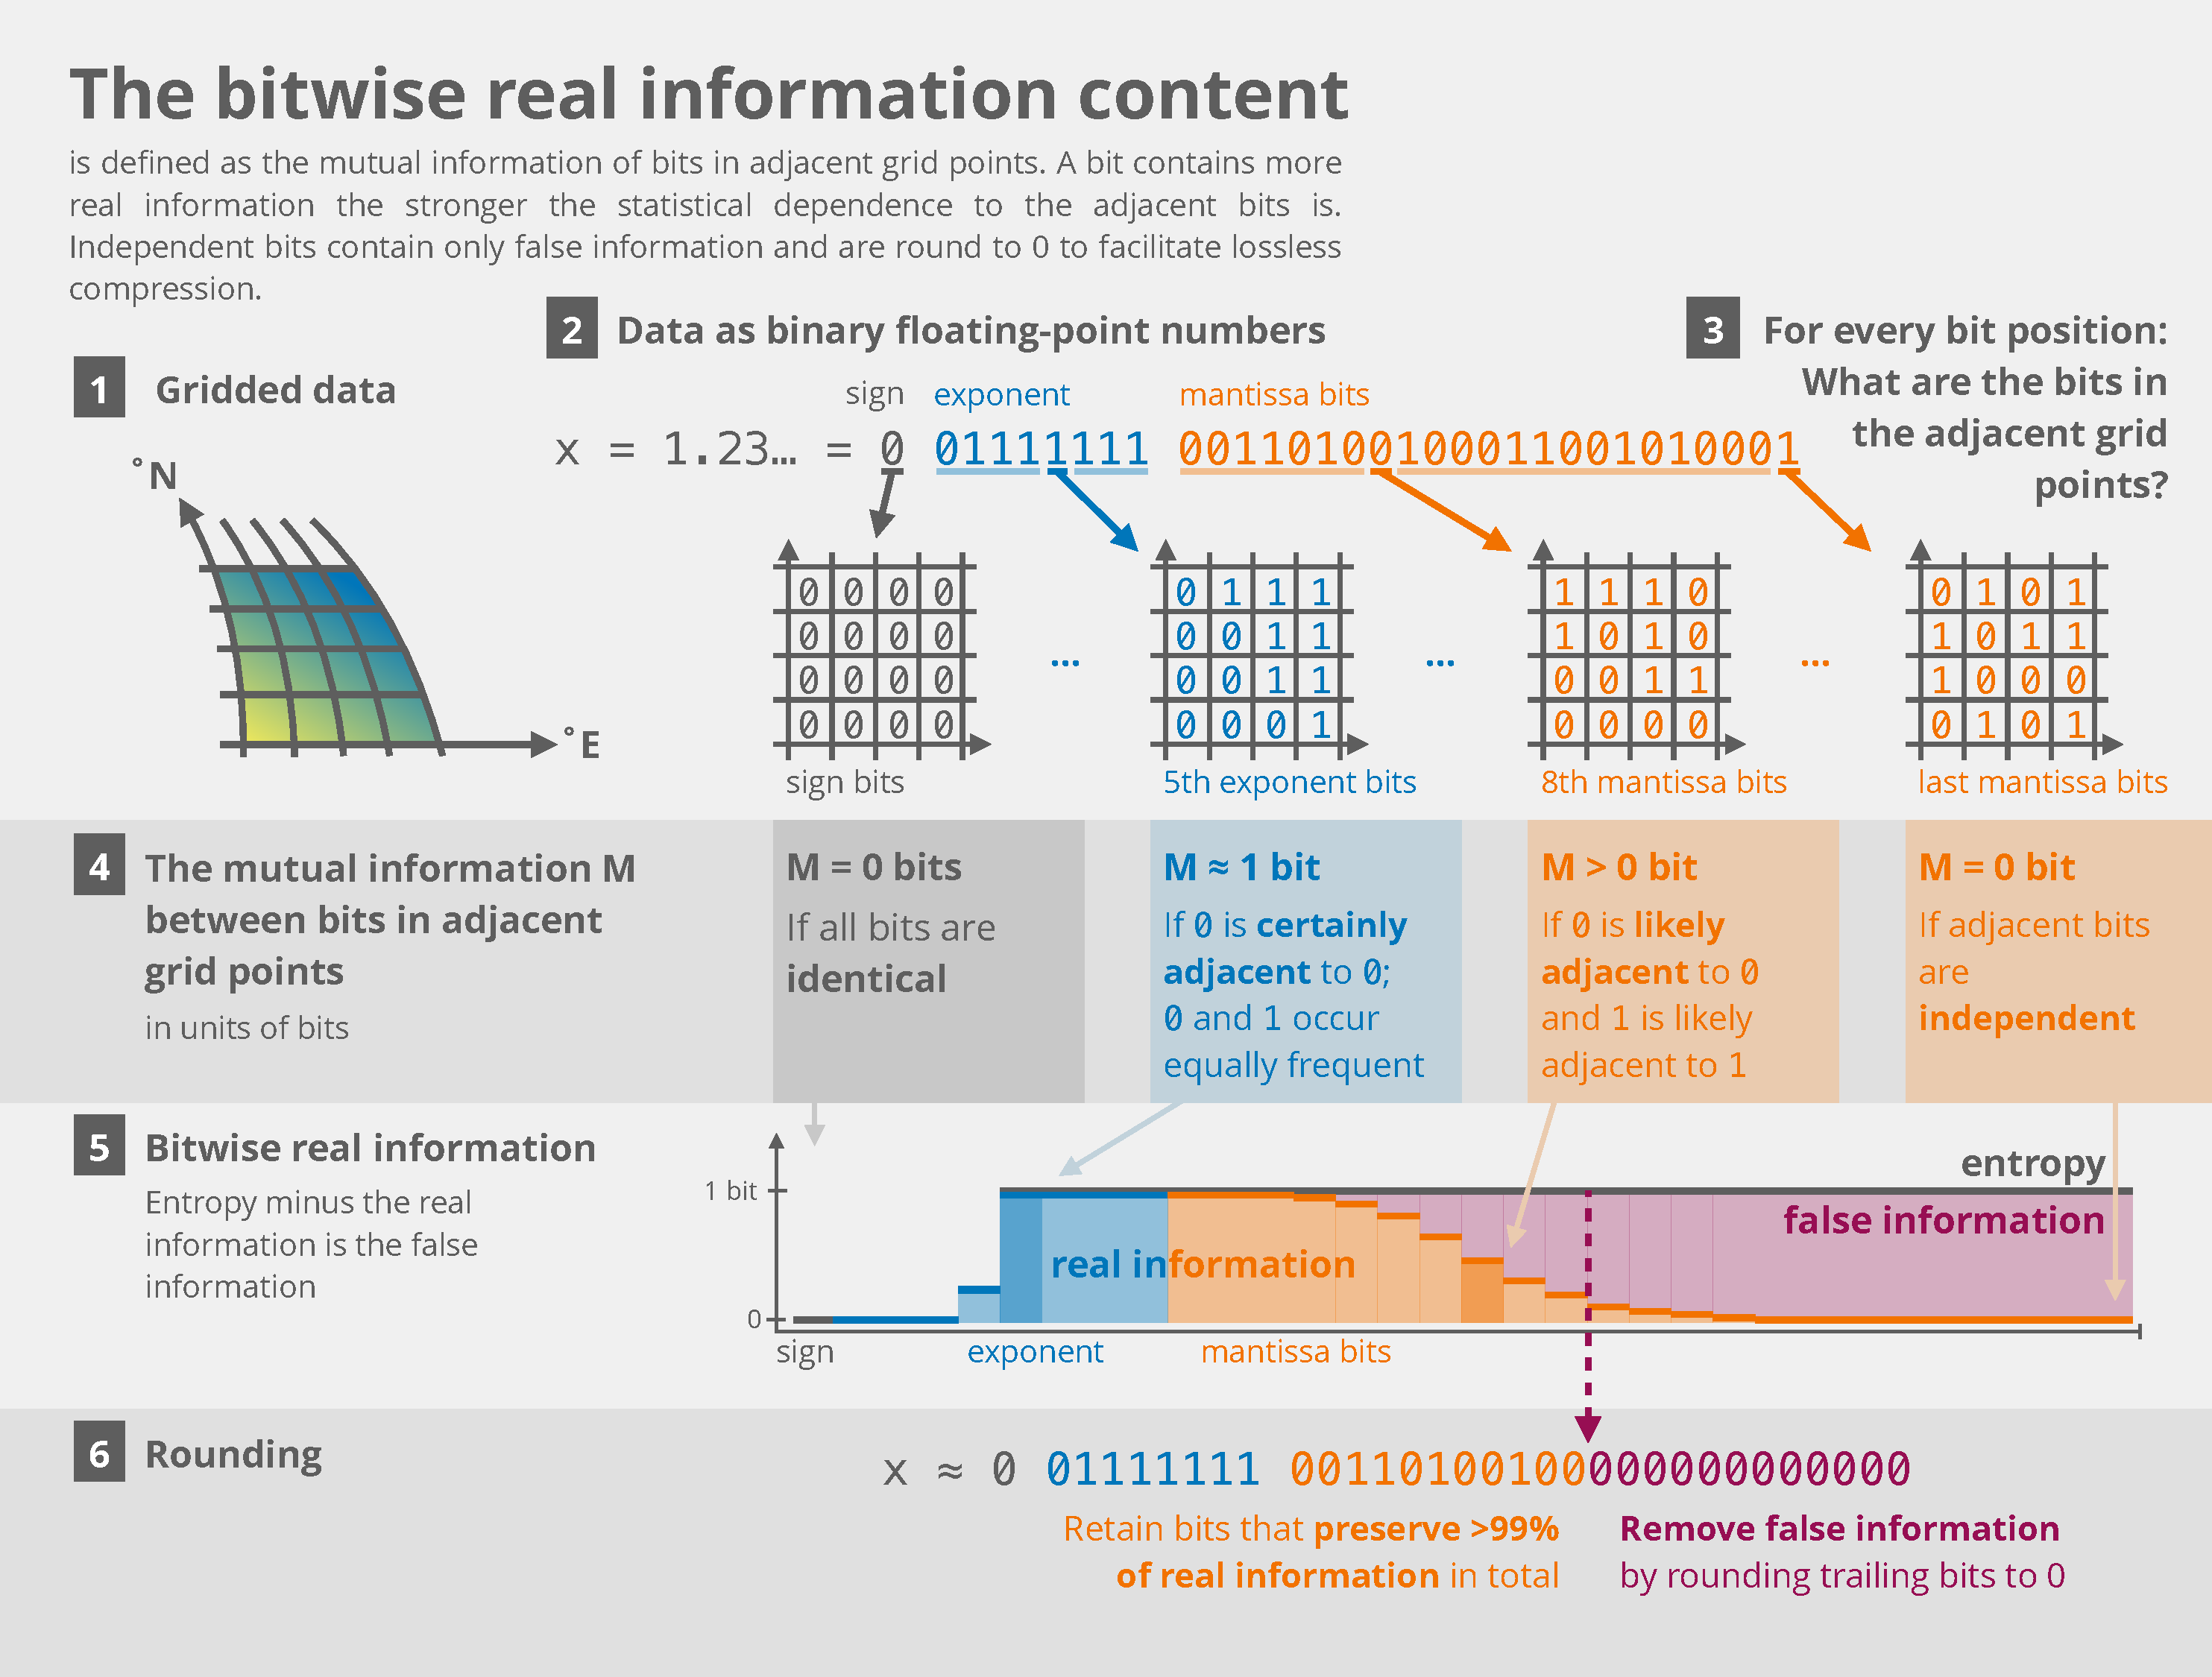
\includegraphics[width=1\textwidth]{Figures/compression/infograph_cut.pdf}
	\caption{\textbf{The bitwise real information content explained schematically.}}
	\label{fig:infograph}
\end{figure}

We define the bitwise real information content as the mutual information
\citep{Shannon1948,MacKay2003,Schreiber2000,Kraskov2004,Pothapakula2019,DelSole2004} of bits in
adjacent grid points (Fig. \ref{fig:infograph}). A bit contains more real information the stronger the statistical
dependence to the adjacent bits is. Bits without real information are identified when this dependence is
insignificantly different from zero and we regard the remaining entropy in these bits as false information.
The adjacent bit can be found in any of the dimensions of the data, e.g. in longitude, time or in the ensemble
dimension. However, always the same bit position is analysed, e.g. the dependence of the first mantissa bit
with other first mantissa bits in adjacent grid points. 

In general, this analysis can be applied to any $n$-dimensional gridded data array when its adjacent elements
are also adjacent in physical space, including structured and unstructured grids. However, data without spatial
or temporal correlation at the provided resolution will be largely identified as false information due to the
independence of adjacent grid points (Fig. \ref{fig:information_resolution} and \ref{fig:information_correlation}).
If valuable scientific information is present in such seemingly random data, then the bitwise real information
content as defined here is unsuited. 

\cite{Jeffress2017} formulate the bitwise information content for simple chaotic systems, assuming an
inherent natural uncertainty which had to be defined. Their approach aims to enable reduced precision
simulations on inexact hardware. Here, we reformulate the bitwise real information as the mutual information
in adjacent grid points for the application in climate data compression. The quantization in the floating-point
representation is used as an uncertainty, such that no additional assumption on the uncertainty of the underlying
data has to be made. While most data compression techniques leave the choice of the retained precision to the user,
the analysis here automatically determines a precision from the data itself based on the separation of real and
false information bits.     

\begin{figure}[tbhp]
	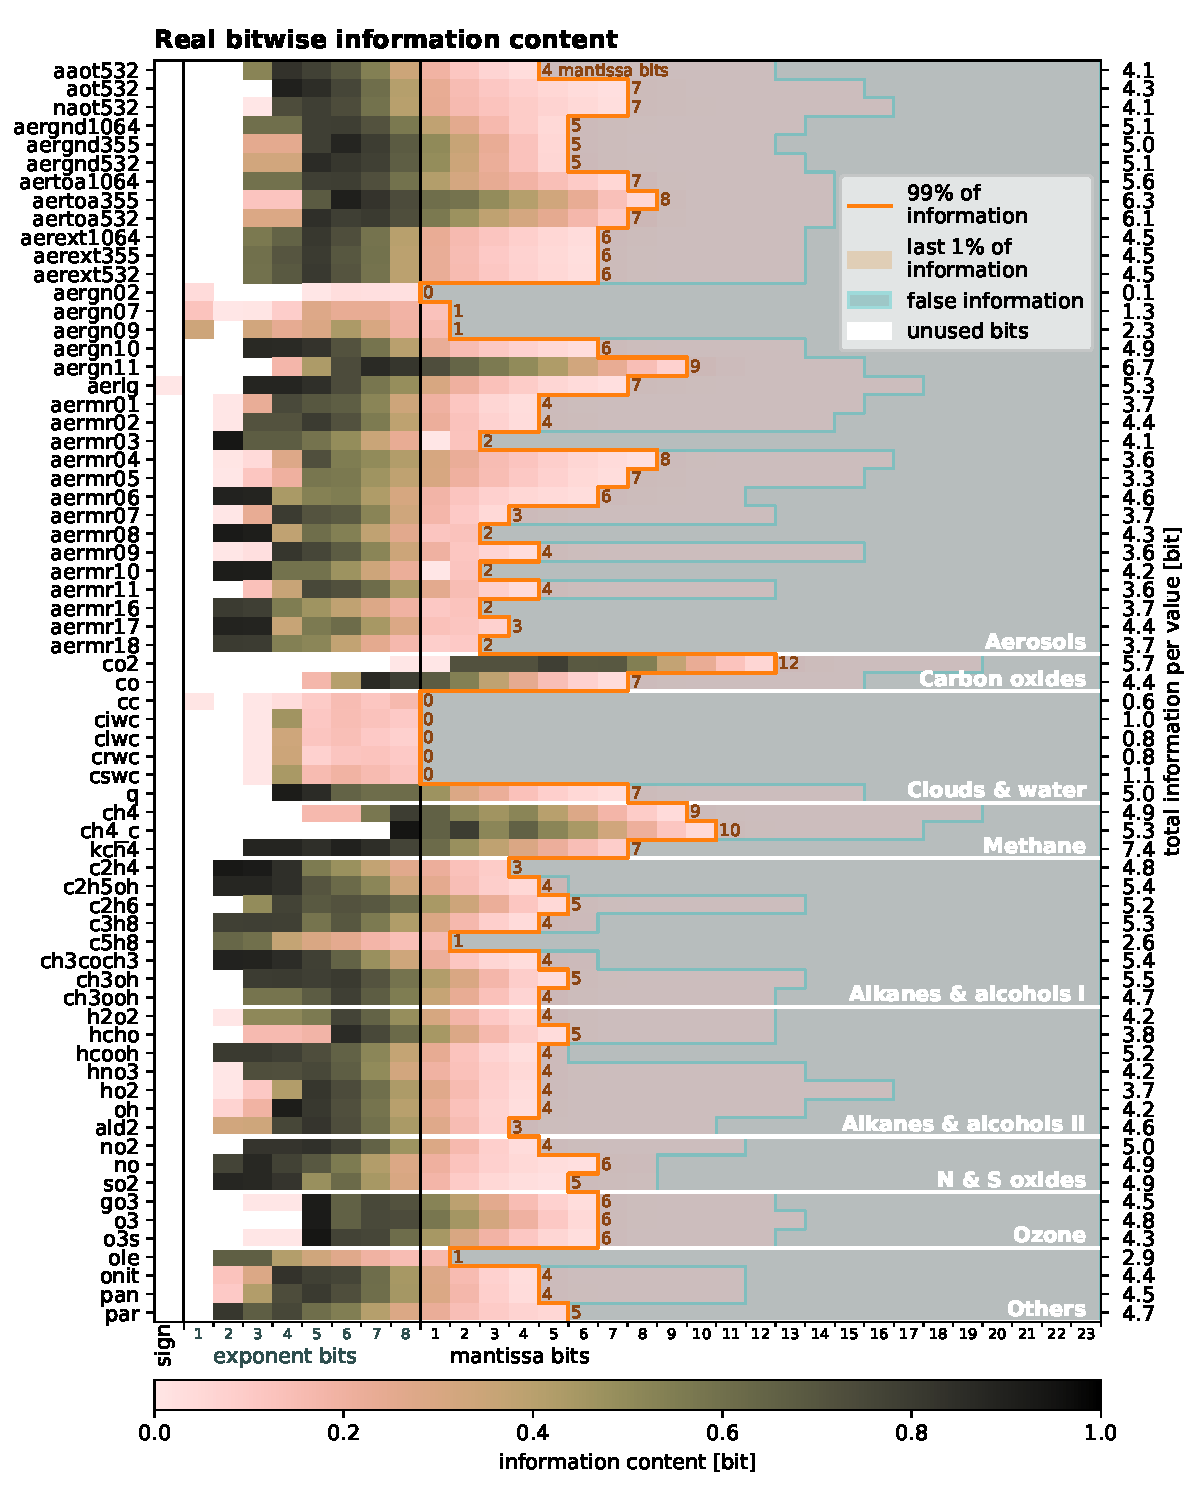
\includegraphics[width=1\textwidth]{Figures/compression/bitinformation.pdf}
	\caption{\textbf{Bitwise real information content for all variables in CAMS.} 
	The real information is calculated in all three spatial dimensions, revealing false information
	and unused bits, using the 32-bit encoding of single-precision floats. The bits that should be
	retained to preserve 99\% of real information are enclosed in orange. Bits without any real
	information are shaded in grey-blue. The sum of the real information across bit positions
	per variable is the total information per value. Variable abbreviations are explained in Table
	\ref{tab:cams_abbreviations}.}
	\label{fig:bitinformation}
\end{figure}

Many exponent bits of the variables in CAMS have a high information content (Fig. \ref{fig:bitinformation}),
but information content decreases to zero within the first mantissa bits for most variables.
Exceptions occur for variables like carbon dioxide (CO\textsubscript{2}) with mixing ratios varying in a very
limited range of 0.5-1.5 mg/kg (equivalent to about 330-990ppmv) globally. Due to the limited range,
most exponent bits are unused and the majority of the real information is in mantissa bits 2 to 12.

The sum of real information across all bit positions is the total information per value, which is less than 7 bits for
most variables. Importantly, the last few percent of total information is often distributed across many mantissa bits.
This presents a trade-off where for a small tolerance in information loss many mantissa bits can be discarded,
resulting in a large increase in compressibility (Fig. \ref{fig:information_error_ssim}a). 
Aiming for 99\% preserved information is found to be a reasonable compromise.

\begin{figure}[tbhp]
	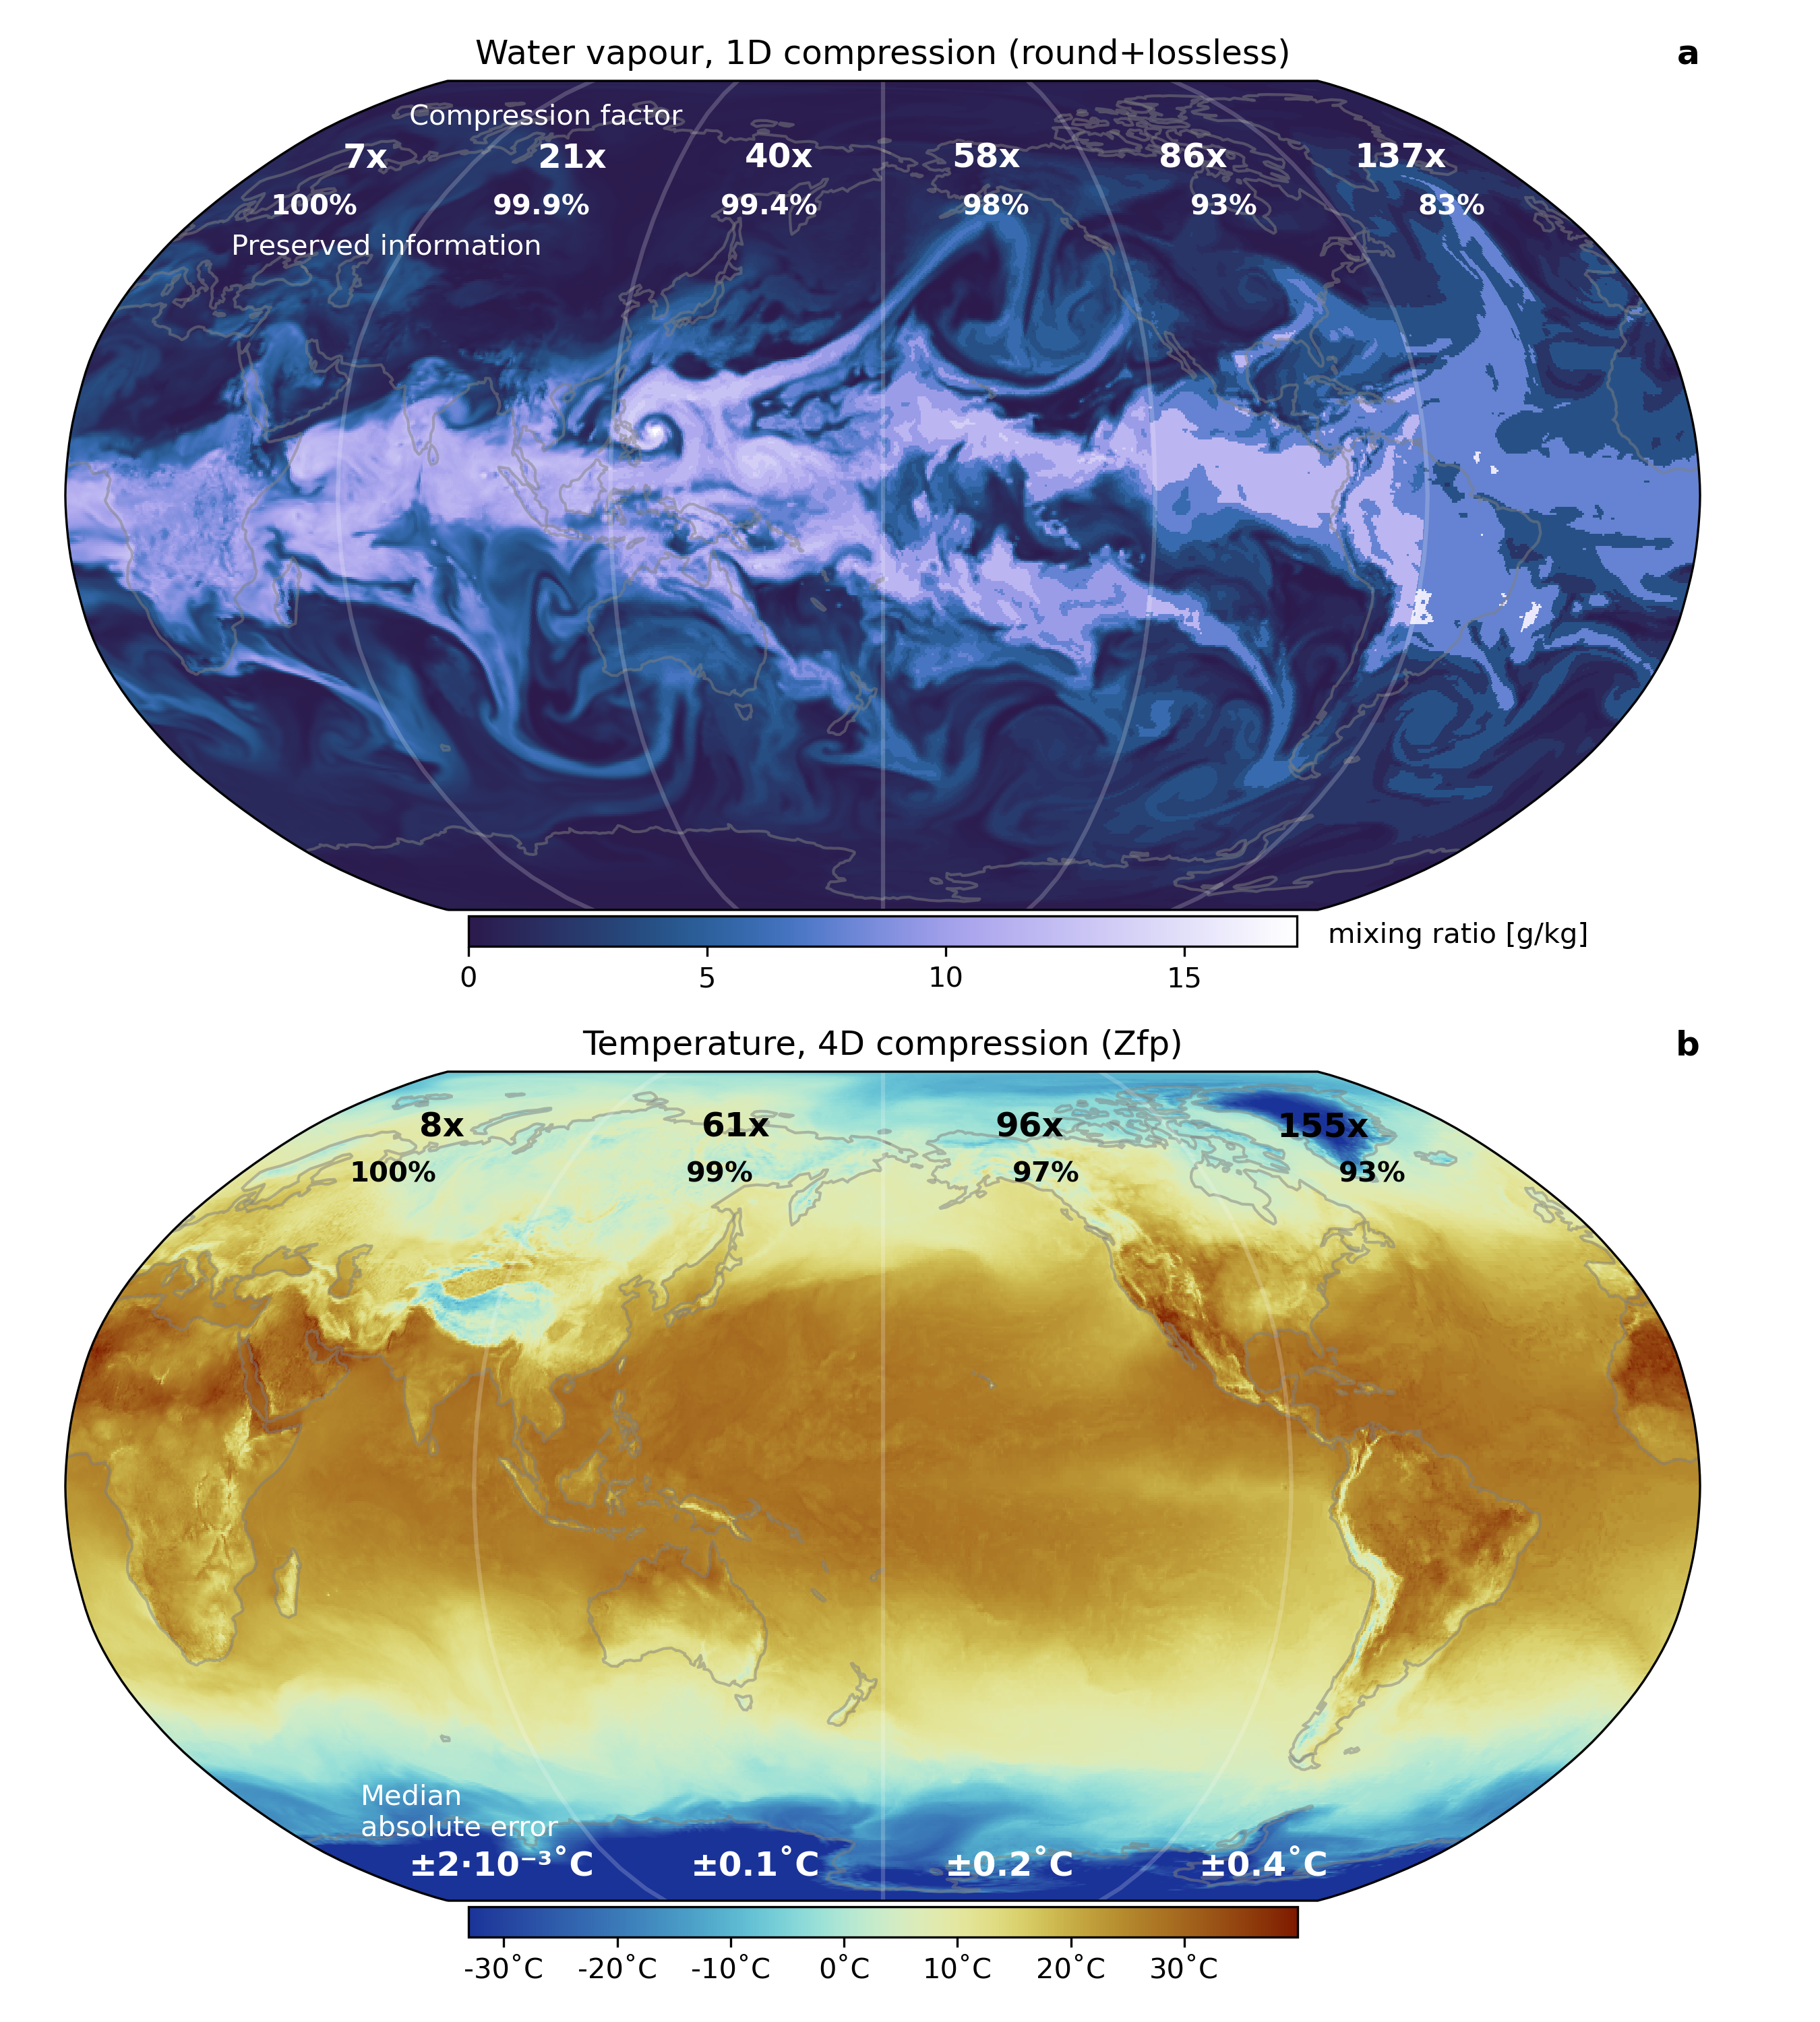
\includegraphics[width=1\textwidth]{Figures/compression/map_water_temp.png}
	\caption{\textbf{Compression at various levels of preserved information. a}
	Water vapour (specific humidity) compressed in the longitudinal dimension. 
	The vertical level shown is at about 2 km geopotential altitude, but compression 
	factors include all vertical levels. \textbf{b} Surface temperature compressed in the
	four space-time dimensions at various levels of preserved information with compression
	algorithm Zfp. Compression factors are relative to 64-bit floats.}
	\label{fig:map_roundlossless_zfp}
\end{figure}

\subsection{Compressing only the real information}

Based on the bitwise real information content, we suggest a new strategy for data compression of climate variables:
First, we diagnose the real information for each bit position. Afterwards, we round bits with no significant real information
to zero, before applying lossless data compression. This allows us to minimise information loss but to maximise the
efficiency of compression algorithms.

Bits with no or only little real information (but high entropy) are discarded via binary round-to-nearest as defined in the
IEEE-754 standard (see section \ref{sec:roundnearest}, \cite{IEEE1985}). This rounding mode is bias-free and therefore
will ensure global conservation of quantities important in climate model data. Rounding removes the incompressible false
information and therefore increases compressibility. While rounding is irreversible for the bits with false information, the
bits with real information remain unchanged and are bitwise reproducible after decompression. Both the real information
analysis and the rounding mode are deterministic, also satisfying reproducibility.

Lossless compression algorithms can be applied efficiently to rounded floating-point arrays (the \emph{round+lossless} method).
Many general-purpose lossless compression algorithms are available
\citep{Ziv1977,Ziv1978,Huffman1952,Delaunay2019,Deutsch1996,Skibinski2020,Alted2010,Collet2020}, which are based on
dictionaries and other statistical techniques to remove redundancies. Most algorithms operate on bitstreams and exploit the
correlation of data in a single dimension only, we therefore describe this method as 1-dimensional (1D) compression. Here, we
use Zstandard for lossless compression \citep{Collet2020}, which has emerged as a widely available default in recent years
(see section \ref{sec:compression_lossless}).

The compression of water vapour at 100\% preserved information (16 mantissa bits are retained) yields a compression
factor of 7x relative to 64-bit floats (Fig. \ref{fig:map_roundlossless_zfp}a). At 99\% of preserved information
(7 mantissa bits are retained) the compression factor increases to 39x. As the last 1\% of real information in water vapour
is distributed across 9 mantissa bits, we recommend this compromise to increase compressibility. With this compression
a 15-fold storage efficiency increase is achieved compared to the current method at 2.67x. Effectively only
1.6 bits are therefore stored per value. 

\begin{figure}[tbhp]
	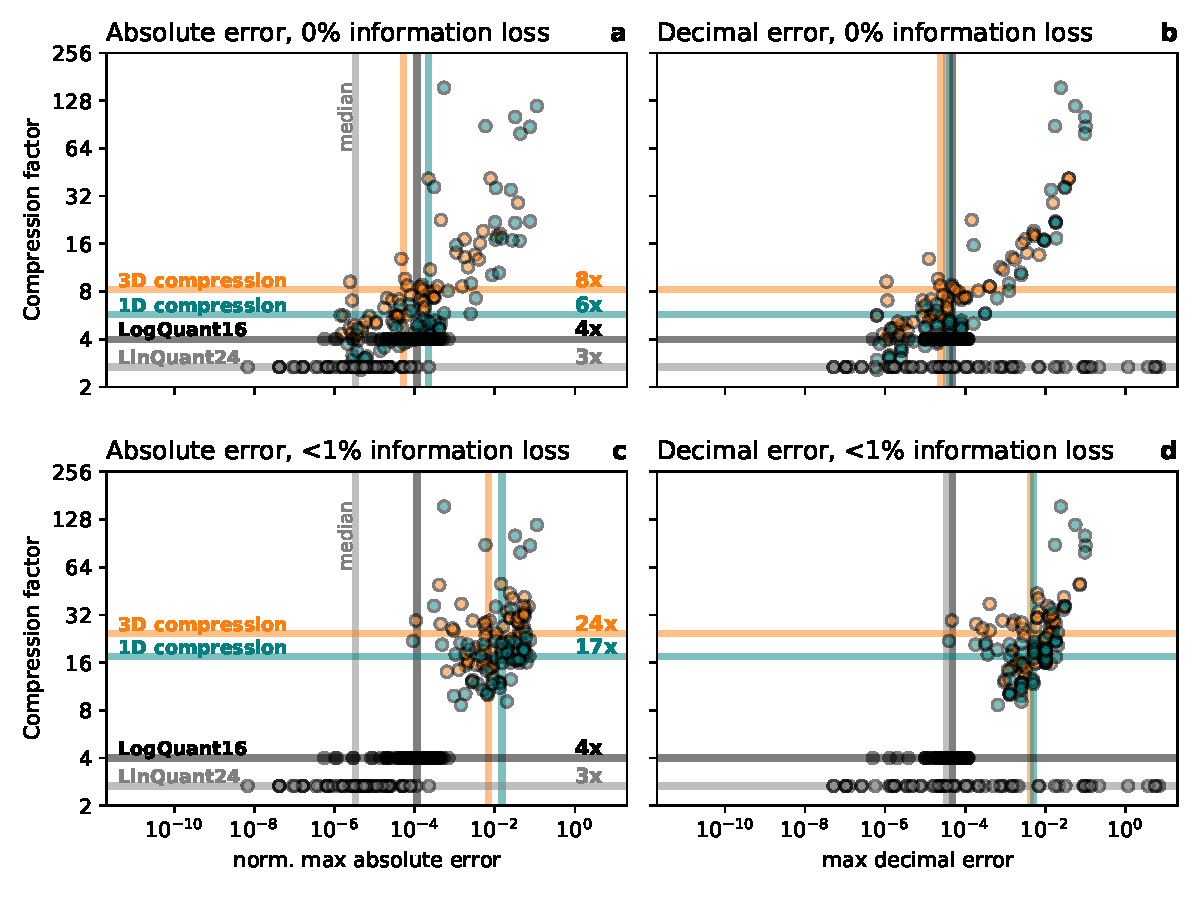
\includegraphics[width=1\textwidth]{Figures/compression/compression_error.pdf}
	\caption{\textbf{Compression factors versus compression errors.} The maximum absolute and decimal error
	for 24-bit linear and 16-bit logarithmic quantization (LinQuant24, LogQuant16) with 1-dimensional round+lossless
	and 3-dimensional Zfp compression. Every marker represents for one variable the global maximum of the \textbf{a, c}
	normalised absolute error, \textbf{b, d} decimal error for \textbf{a, b} 100\% preserved information, and \textbf{c, d}
	 99\% preserved information. The geometric mean of compression factors over all variables is given as horizontal lines.
	 The median of the errors across all variables is given as vertical lines.}
	\label{fig:compression_error}
\end{figure}

Compressing all variables in CAMS and comparing error norms reveals the advantages of the 1D round+lossless method
compared to the 24-bit linear quantization technique currently in use (Fig. \ref{fig:compression_error}). The maximum decimal
errors (see section \ref{sec:decimal_precision}) are smaller for many variables due to the logarithmic distribution of floating-point numbers.
Some variables are very compressible (>60x) due to many zeros in the data, which is automatically made use of in the lossless compression.
Compression factors are between 3x and 60x for most variables, with a geometric mean of 6x when preserving 100\% of information.
Accepting a 1\% information loss the geometric mean reaches 17x, which is the overall compression factor for the entire CAMS data
set with this method when compared to data storage with 64 bits per value.

Furthermore, the 24-bit linear quantization could be replaced by a 16-bit logarithmic quantization, as the mean and absolute errors
are comparable. The decimal errors are often even lower and naturally bound in a logarithmic quantization despite fewer available bits.

\begin{figure}[tbhp]
	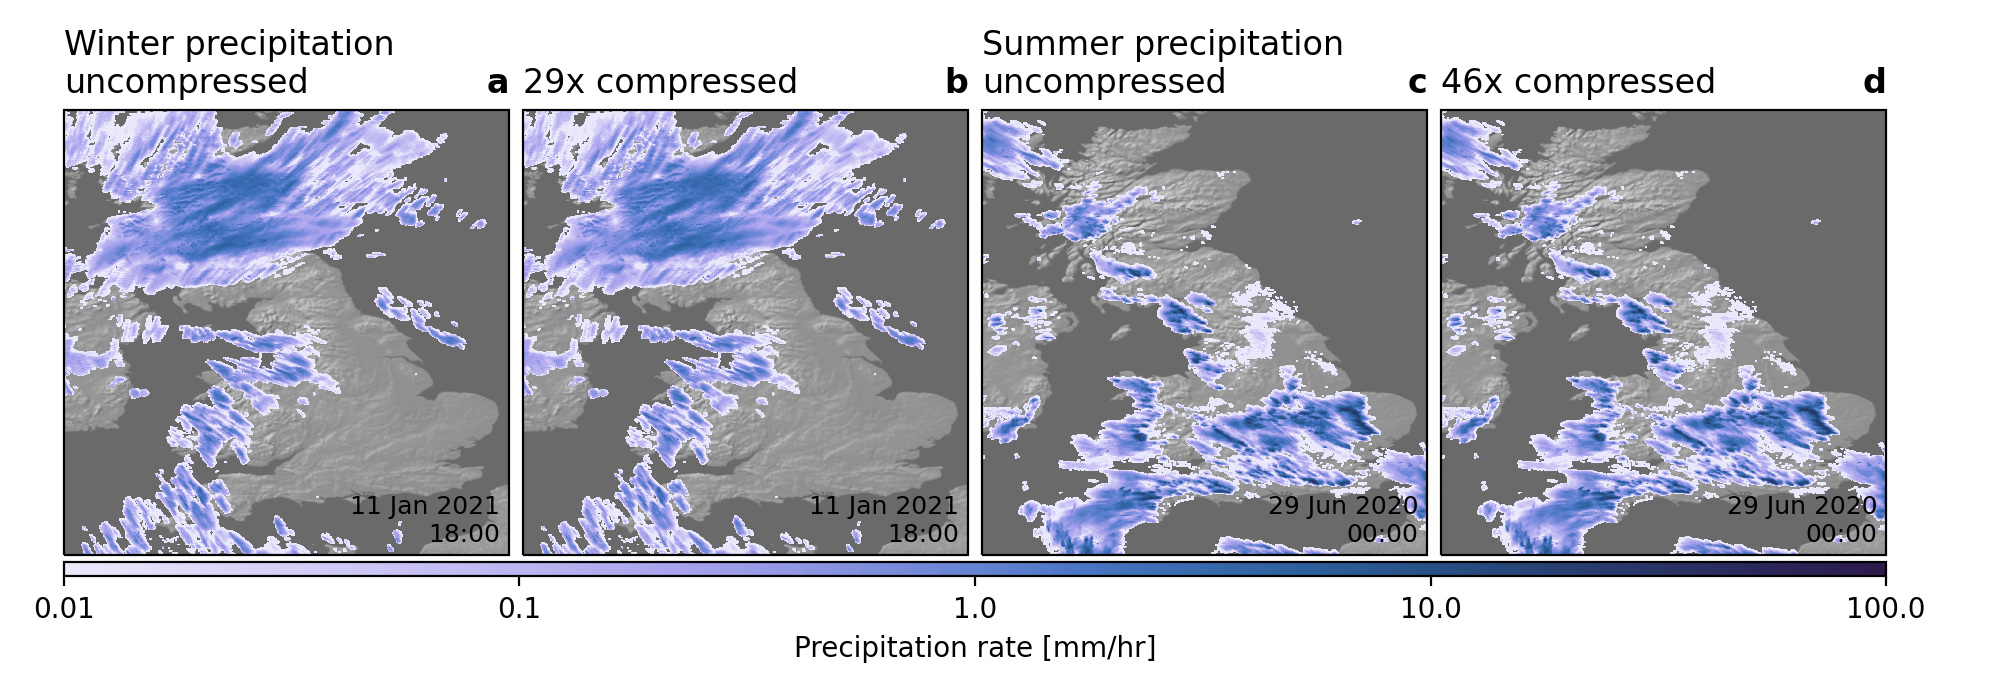
\includegraphics[width=1\textwidth]{Figures/compression/precipitation_compression.png}
	\caption{\textbf{Compression of radar-based observations of precipitation over Great Britain. a}
	Precipitation for the hour preceding 18:00 UTC on 11 Jan 2021 from the UK MetOffice NIMROD data at about 1km
	horizontal resolution. \textbf{b} as a but the data was compressed preserving 99\% of real information achieving
	compression factors of 29x relative to 64 bit. \textbf{c} and \textbf{d} as \textbf{a} and \textbf{b} but for 00:00 UTC
	on 29 Jun 2021 and achieving compression factors of 46x.}
	\label{fig:precipitation}
\end{figure}

A broad applicability of the bitwise real information content analysis for compression is tested with further data sets:
Radar-based observations of precipitation over Great Britain are similarly compressible using the same method
(Fig. \ref{fig:precipitation}) and so are satellite measurements of brightness temperature with a very high resolution
of about 300m horizontally (Fig. \ref{fig:brightness_temp}). Even for anthropogenic emissions of methane or nitrogen
dioxide similar compression results are obtained, despite limited spatial correlation of point sources (Fig. \ref{fig:methane_no2}).
The bitwise real information content in this case is largely determined by the smooth background concentrations and
therefore still sufficiently high to preserve the point sources. 

In an operational setting we recommend the following workflow: First, for each variable the bitwise real information
content is analysed from a representative subset of the data. Representative is, for example, a single time step for
subsequent time steps if the statistics of the data distribution are not expected to change. From the bitwise real information
the number of mantissa bits to preserve 99\% of information is determined  (the \emph{keepbits}). Second, during the simulation the
arrays that will be archived are rounded to the number of keepbits (which are held fixed) and compressed. The first step
should be done offline, meaning once in advance of a data-producing simulation. Only the second step has to be performed
online, meaning every time data is archived. 

\begin{figure}[tbhp]
	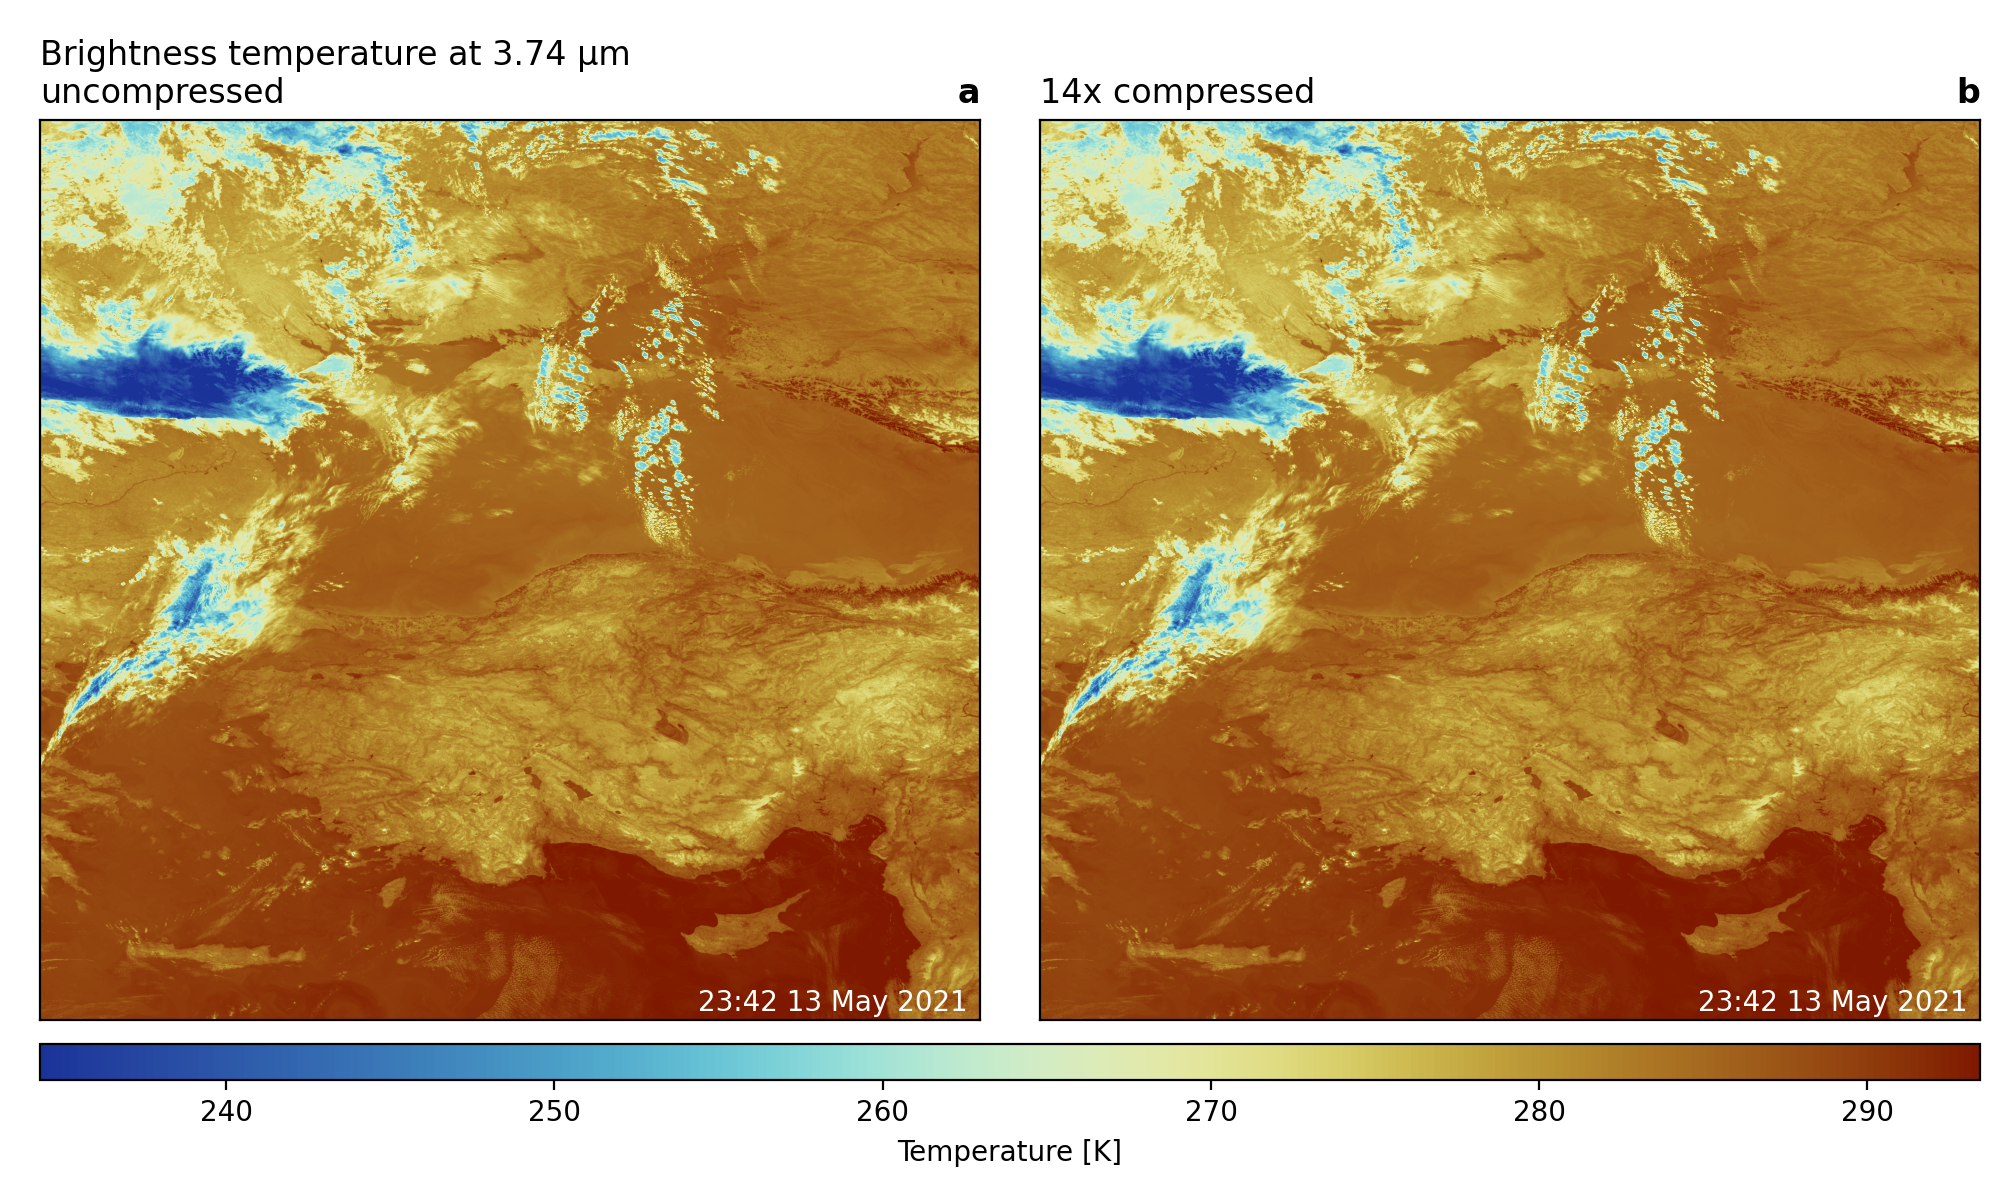
\includegraphics[width=1\textwidth]{Figures/compression/brightness_temp.png}
	\caption{\textbf{Compression of satellite-based observations of brightness temperature over the
	Black Sea and Turkey. a} Brightness temperature measured by the 3.74\textmu m (I4) channel of
	the VIIRS sensor on board the Suomi-NPP satellite at about 300m horizontal resolution on
	the 13 May 2021. \textbf{b} as \textbf{a} but the data was compressed preserving 99\% of
	real information with the round+lossless method achieving compression factors of 14x
	relative to 64 bit.}
	\label{fig:brightness_temp}
\end{figure}

The presented round+lossless compression technique separates the lossy removal of false information and the actual lossless
compression. This provides additional flexibilities as any lossless compressor can be used and application-specific choices can
be made regarding availability, speed and resulting file sizes. However, most general-purpose lossless compression algorithms
operate on bitstreams and require multidimensional data to be unravelled into a single dimension. Multidimensional correlation
is therefore not fully exploited in this approach.

\begin{figure}[tbhp]
	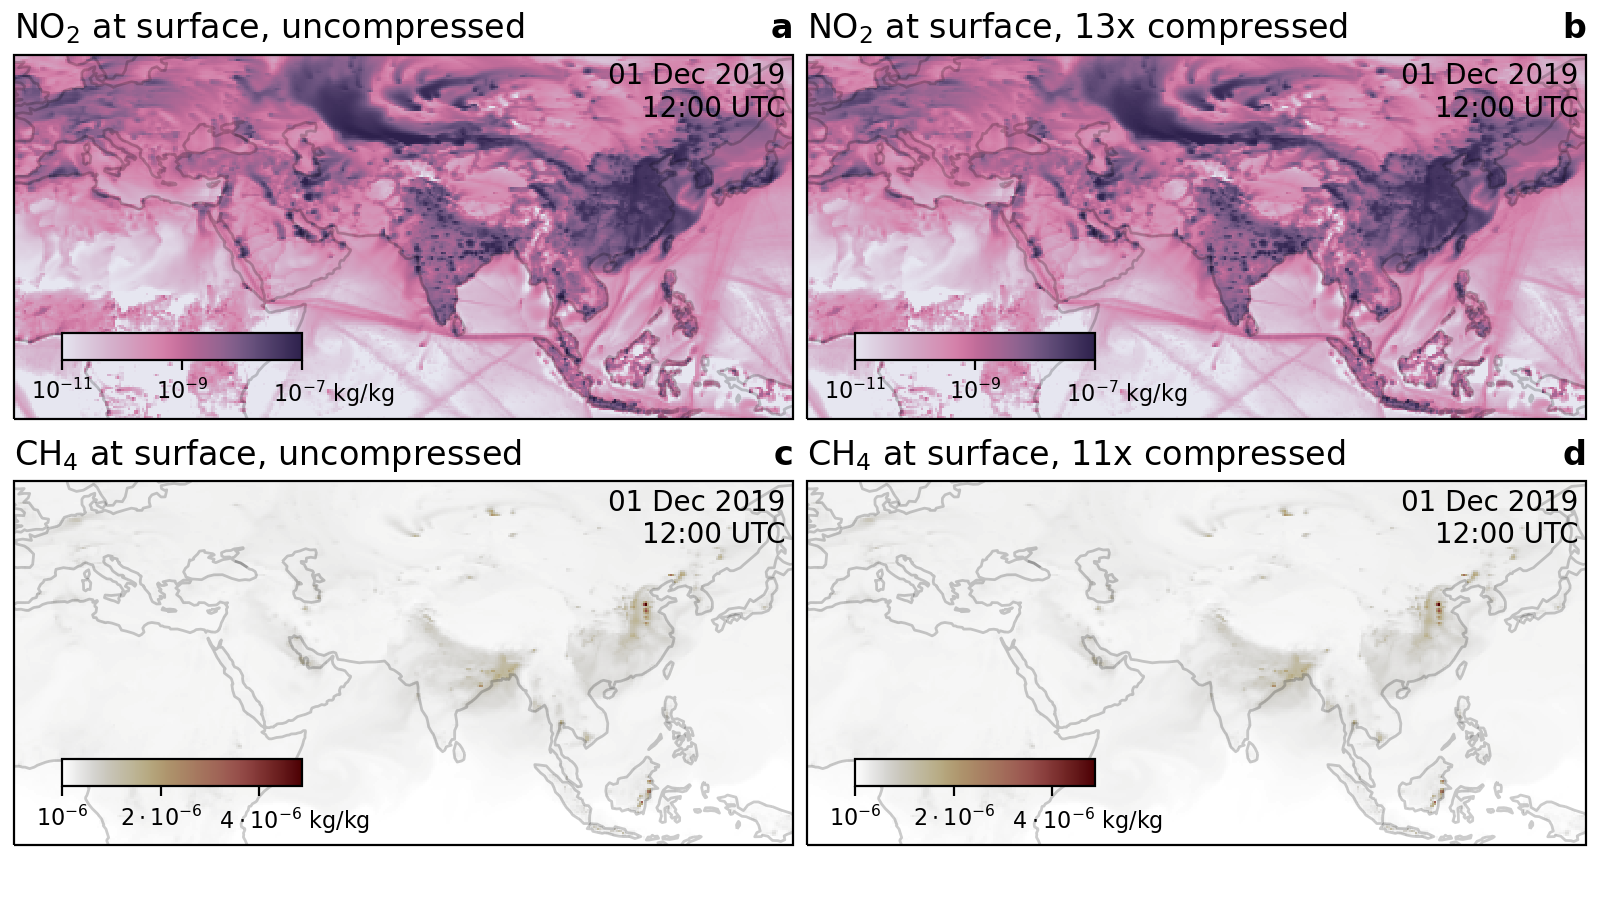
\includegraphics[width=1\textwidth]{Figures/compression/methane_no2_surface.png}
	\caption{\textbf{Compression of nitrogen dioxide (NO\textsubscript{2}) and methane (CH\textsubscript{4}) at the surface. a}
	Surface NO\textsubscript{2} concentrations preliminary result from fossil fuel combustion. \textbf{b} Surface CH\textsubscript{4}
	concentrations often include point sources, such as here in East China, East India and East Borneo. 
	\textbf{b,d} as \textbf{a,c} but compressed preserving 99\% of information achieving a compression factor of 13x, 11x,
	respectively.}
	\label{fig:methane_no2}
\end{figure}

We extend the ideas of information-preserving compression to modern multidimensional compressors. The analysis of the bitwise
real information content leads naturally to the removal of false information via rounding in the round+lossless method. For other
lossy compressors, however, the separation of real and false information has to be translated to the precision options of such
compressors. While such a translation is challenging in general, we present results from combining the bitwise real information
analysis with one modern multidimensional compressor in the next section.

\subsection{Multidimensional climate data compression}

Modern compressors have been developed for multidimensional floating-point arrays
\citep{Lindstrom2006,Di2016,Ballester-Ripoll2020,Zhao2020,vonLarcher2019}, which compress in
several dimensions simultaneously. We will compare the 1D round+lossless compression to Zfp, a modern compression
algorithm for two to four dimensions \citep{Lindstrom2014,Pinard2020,Poppick2020,Hammerling2019}.
Zfp divides a $d$-dimensional array into blocks of $4^d$  values (i.e. the edge length is 4), which allows to
exploit the correlation of climate data in up to 4 dimensions. To extend the concept of information-preserving
compression to modern compressors like Zfp, the bitwise real information is translated to the precision options of Zfp
(more details in section \ref{sec:zfp_compression}).

\begin{figure}[tbhp]
	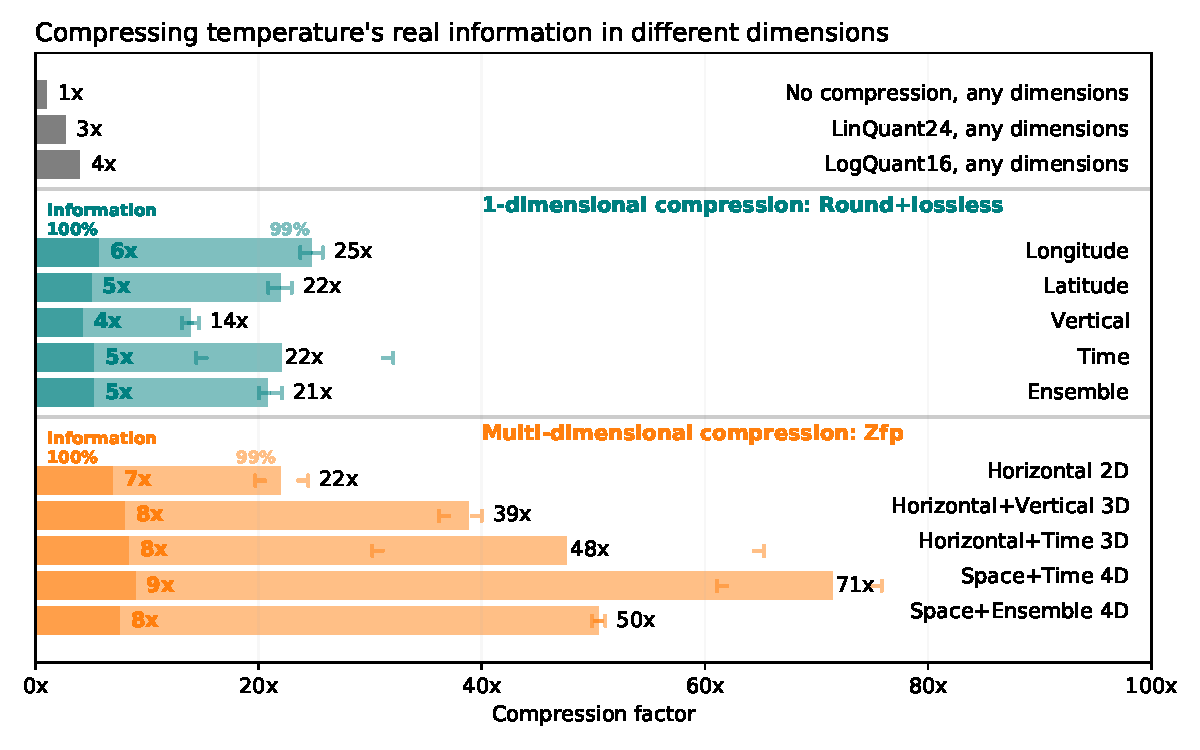
\includegraphics[width=1\textwidth]{Figures/compression/compressfac_comparison.pdf}
	\caption{\textbf{Multidimensional compression allows for higher compression factors.}
	\mbox{1-dimensional} compression (round+lossless) of temperature reaches at most 25x when preserving 99\% 
	of real information with the round+lossless method, whereas 71x is reached with 4-dimensional (4D)
	space-time compression using Zfp compression. Preserving 100\% of information considerably lowers
	the compression factors to 4-9x. Error brackets represent the min-max range of compression when
	applied to various data samples.}
	\label{fig:compressfac_comparison}
\end{figure}

Multidimensional compression imposes additional inflexibilities for data retrieval: Data is compressed and decompressed
in larger chunks, which can increase the load on the data archive. For example, if the data is compressed across the time
dimension, data of several time steps have to be downloaded and decompressed although only data from a single time
step might be requested. Downloads from an archive might therefore increase if the data chunking is not well suited to
typical data requests from users. 

For 1D compression the compressibility varies with the dimension: Longitude (i.e. in the zonal direction) is more compressible,
reaching 25x for temperature at 99\% preserved information, than compressing in the vertical which yields only 14x
(Fig. \ref{fig:compressfac_comparison}). This agrees with the predominantly zonal flow of the atmosphere as spatial
correlation in the zonal direction is usually highest. For a constant number of retained mantissa bits, higher resolution
in the respective dimensions increases the compressibility as also the correlation in adjacent grid points increases
(Fig. \ref{fig:information_resolution} and \ref{fig:information_correlation}).

For multidimensional compression it is generally advantageous to include as many highly correlated dimensions as possible.
In that sense, including the hourly-resolved forecast lead time instead of the vertical dimension in 3D compression yields
higher compression factors. 4D space-time compression is the most efficient, reaching 60-75x at 99\% preserved information.
For temperature this is equivalent to a median absolute error of 0.1\textdegree{}C (Fig. \ref{fig:map_roundlossless_zfp}b).

\begin{figure}[tbhp]
	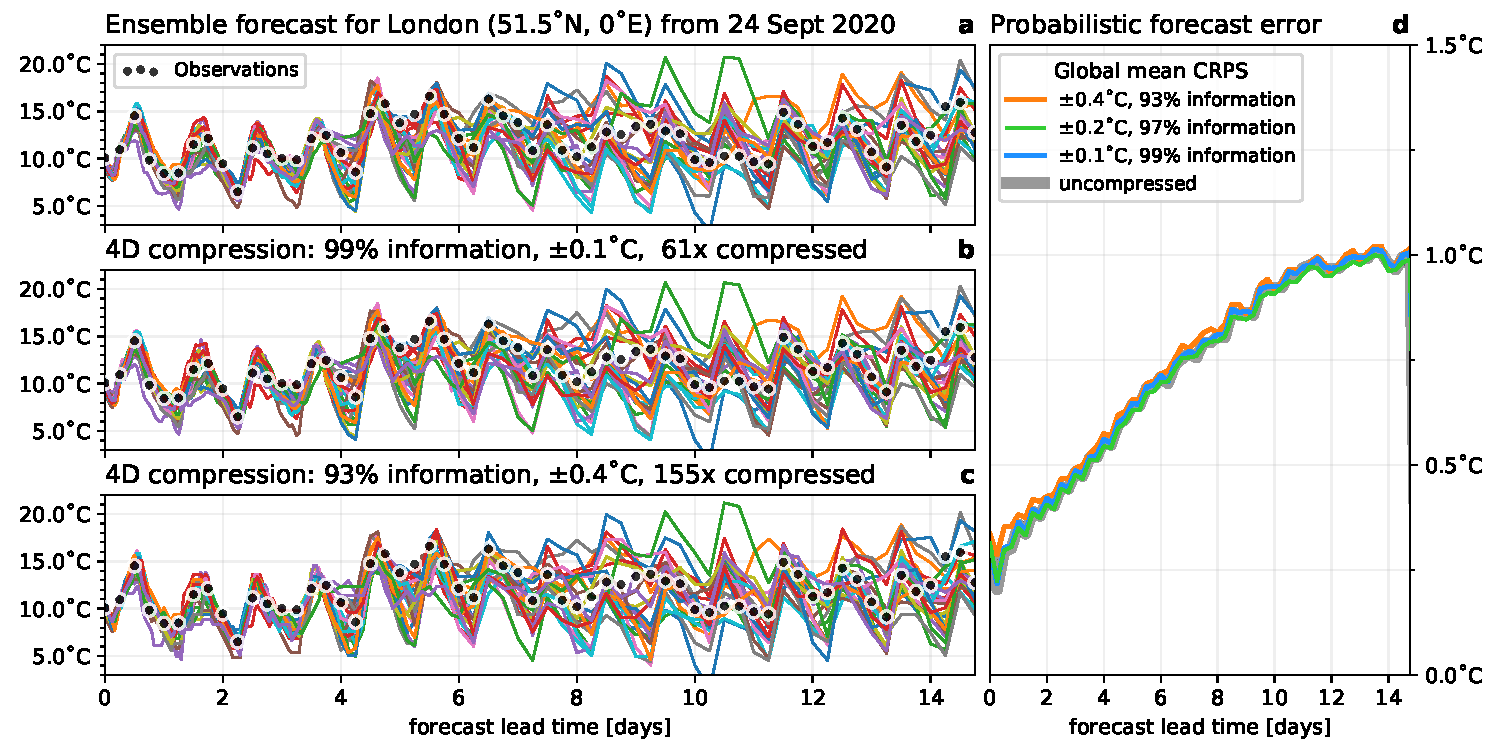
\includegraphics[width=1\textwidth]{Figures/compression/ensemble_forecast.pdf}
	\caption{\textbf{Verification of an ensemble forecast with the probabilistic forecast error based on ensemble data
	with and without compression. a} 25-member uncompressed ensemble forecast (lines) of surface temperature
	in London, UK from 24 Sept 2020 up to 15 days ahead. \textbf{b} as a but the data was compressed in 4-dimensional
	(4D) space-time with Zfp, preserving 99\% of real information. \textbf{c} as \textbf{b} but only preserving 93\% of real
	information. \textbf{d} Probabilistic forecast error (continuous ranked probability score, CRPS) for various levels of
	preserved information in the compression. The CRPS does not increases relative to the uncompressed reference for
	more than 93\% of preserved information.}
	\label{fig:ensemble_forecast}
\end{figure}

Compressing the entire CAMS dataset in the three spatial dimensions with Zfp while preserving 99\% of the information yields
an overall compression factor of 24x (Fig. \ref{fig:compression_error}). Maximum absolute error and decimal errors are for
most variables very similar to 1D round+lossless (see Fig. \ref{fig:compression_error_distribution} and section
\ref{sec:zfp_compression} for a discussion why they are not identical), providing evidence that a
multidimensional compression is preferable for higher compression factors. 

Due to the limited meaning of error norms in the presence of uncertainties in the uncompressed reference data, the forecast
error is assessed to quantify the quality of compressed atmospheric data. The continuous ranked probability score
(CRPS, \cite{Matheson1976,Hersbach2000,Zamo2018}),
a generalisation of the root-mean-square error for probabilistic forecasts, is evaluated for global surface temperature using observations
every 6 hours as truth (Fig. \ref{fig:ensemble_forecast}). Compared to the uncompressed data, no significant increase of the CRPS forecast error 
occurs for individual locations or globally at 99\% and 97\% preserved information. The usefulness for the end user of the global temperature
forecast is therefore unaltered at these levels of preserved information in the compression. Contrarily, with an information loss larger than
5\% the CRPS forecast error starts to increase, while large compression factors beyond 150x are achieved.

\begin{figure}[tbhp]
	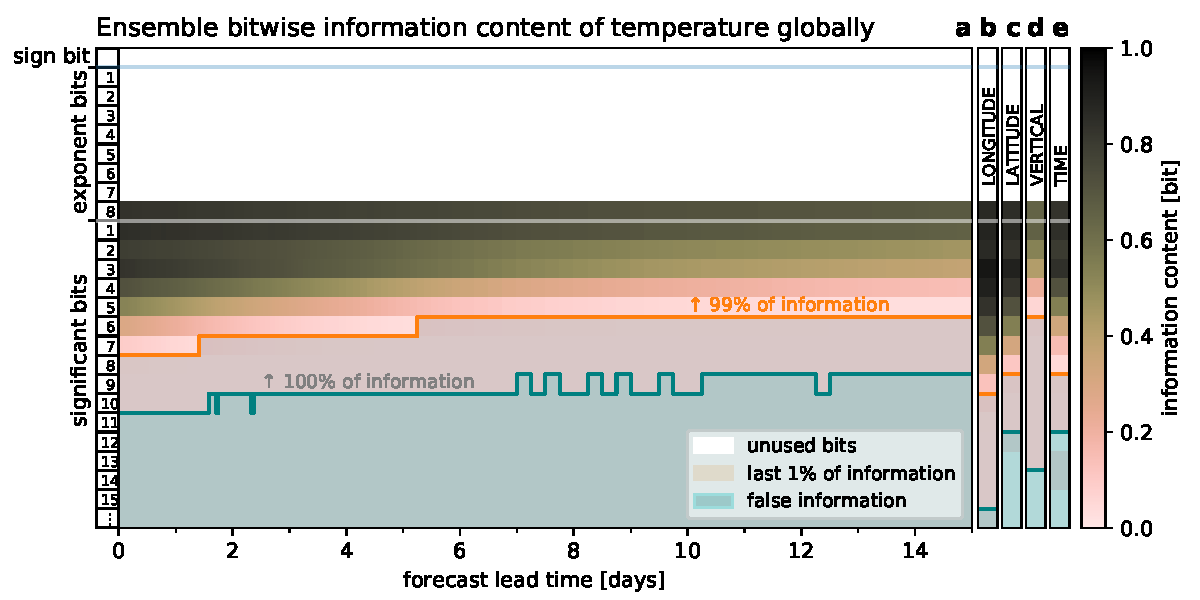
\includegraphics[width=1\textwidth]{Figures/compression/ensemble_information.pdf}
	\caption{\textbf{Bitwise real information content for temperature in various dimensions. a} ensemble, \textbf{b} longitude,
	\textbf{c} latitude, \textbf{d} vertical and \textbf{e} forecast lead time. The ensemble information effectively encodes the
	ensemble mean, which is less information than in most other dimensions. Longitude, latitude and forecast lead time
	have the highest total information which should be preserved in compression. The ensemble information decreases
	over time as the ensemble spread increases (Fig. \ref{fig:ensemble_forecast}).}
	\label{fig:ensemble_information}
\end{figure}

\subsection{A Turing test for data compression}

In numerical weather predictions, progress in the development of global weather forecasts is often assessed using a set of error metrics,
summarised in so-called \emph{score cards}. These scores cover important variables in various large scale regions, such as the temperature
2m above the surface over Europe or horizontal wind speed at different vertical levels in the Southern Hemisphere. With a similar motivation
as in \cite{Baker2019}, we suggest assessing the efficiency of climate data compression using similar scores, which have to be passed similar
to a Turing test \citep{Baker2016,Turing1950}. The compressed forecast data should be indistinguishable from the uncompressed data in all
of these score tests, or at least indistinguishable from the current compression method while allowing higher compression factors.  Many score
tests currently in use represent area-averages (such as Fig. \ref{fig:ensemble_forecast}d), which would also be passed with coarse-grained data
-- reducing the horizontal resolution from 10km to 20km, for example, yields a compression factor of 4x. It is therefore
important to include resolution-sensitive score tests such as the maximum error in a region. 

A Turing test for data compression could be used iteratively to optimise the level of preserved information in compression. Such an iteration could be 
formulated as follows

\begin{enumerate}
	\item Create 4 seemingly identical data sets with
		\begin{itemize} 
			\item[\texttt{FULL}] Full precision, i.e. no lossy compression was applied
			\item[\texttt{CURR}] Current compression method
			\item[\texttt{INF0}] Conservative information-preserving compression, e.g 99\%
			\item[\texttt{INF1}] Progressive information-preserving compression, e.g. 98\%
		\end{itemize}
	\item Disseminate \texttt{FULL}, \texttt{CURR}, \texttt{INF0}, and \texttt{INF1}  to users, then
		\begin{enumerate}[i]
			\item if \texttt{FULL}, \texttt{CURR}, \texttt{INF0}, and \texttt{INF1} are indistinguishable,
			define \texttt{INF1} as the new \texttt{INF0} and preserve less information in \texttt{INF1}, e.g. 97\% instead of 98\%
			\item if \texttt{CURR} is identified as least useful, conclude that information-preserving should be considered as
			the new default compression method and continue to i
			\item if \texttt{INF1} or \texttt{INF0} are identified as least useful, define \texttt{INF0} as the new \texttt{INF1} and
			preserve more information in \texttt{INF0}, e.g . 99.5\% instead of 99\%
		\end{enumerate}
	\item Reiterate from 1.
\end{enumerate}

While a compression method either passes or fails a conventional Turing test, there is additional value in conducting such a test.
Evaluating the failures will highlight problems and evaluating the passes may identify further compression potential. An iterative Turing test
as presented here can be used to translate an abstract property of data such as usefulness to users into a compression level (here \% of
preserved information).

\section{Discussion}
\label{sec:compression_discussion}

While weather and climate forecast centres produce very large amounts of data, especially for future cloud and storm-resolving models,
only the real information content in this data should be stored. We have here presented a methodology to identify real and false information
in atmospheric, and more generally, climate data. This novel information-preserving compression relies on the removal of false information
via rounding and can then be used in combination with any lossless compression algorithm. Applied to CAMS data we show that a high
compressibility can be achieved without increasing the forecast error. The entire data set is 17x smaller in the compressed form when
compared to 64-bit values but preserves 99\% of the real information. This is about 6-times more efficient when compared to the
current compression method.

Alternatively, the analysis of the bitwise real information content can be used to inform multidimensional compressors. Ideally, climate data
compression should exploit correlation in as many dimensions as possible for highest compression factors. The most important dimensions
to compress along are longitude, latitude and time, which provide the highest compressibility. With Zfp we achieve factors of 60-75x for
4D space-time compression of temperature while preserving 99\% of real information and without increasing forecast errors. Using the three
spatial dimensions the entire set of variables in CAMS data can be compressed by 24x equivalently.

No additional uncertainty measure has to be assumed for the distinction of real and false information presented here. The uncertainty of a variable
represented in a data array is directly obtained from the distribution of the data itself. Most lossy compression techniques leave the choice of
precision to the user, which may lead to subjective choices or the same precision for a group of variables. Instead, our suggestion that
99\% of information should be preserved may be altered by the user, which will implicitly determine the required precision for each variable individually. 

To be attractive for large data sets, a compression method should enable compression as well as decompression at reasonable speeds.
ECMWF produces data at about 2GB/s, including CAMS which creates about 15 MB/s. Data on ECMWF’s archive is compressed once,
but downloaded on average at 120 MB/s by different users, such that both high compression and decompression speeds are important.
The (de)compression speeds obtained here are all at least 100MB/s single-threaded, but faster speeds
are available in exchange for lower compression factors (Fig. \ref{fig:compression_speed}). The real information is only analysed once
and ultimately independent of the compressor choice.

Lossy compression inevitably introduces errors compared to the uncompressed data. Weather and climate forecast data, however,
already contains uncertainties which are in most cases larger than the compression error. For example, limiting the precision of
surface temperature to 0.1\textdegree{}C (as shown in Fig. \ref{fig:map_roundlossless_zfp}b) is well below the average forecast error
(Fig. \ref{fig:ensemble_forecast}d) and also more precise than the typical precision of 1\textdegree{}C presented to end users of a
weather forecast. Reducing the precision to the real information content does not just increase compressibility but also helps to
directly communicate the uncertainty within the data set — an important, often neglected, information by itself.

Satisfying requirements on size, precision and speed simultaneously is an inevitable challenge of data compression. As the precision
can be reduced without losing information, we revisit this trade-off and propose an information-preserving compression. While current
archives likely use large capacities to store random bits, the analysis of the bitwise real information content is essential towards
efficient climate data compression.

\newpage
\section{Appendix}
\begin{table}[htbp]
	\center
	\footnotesize
	\begin{tabular}{l | l | l | l | l | l}
	\textbf{Name} & \textbf{Code} & \textbf{Unit} & \textbf{Name} & \textbf{Code} & \textbf{Unit} \\
	\hline
	\multicolumn{3}{l}{\textbf{Aerosols}} & \multicolumn{3}{l}{\textbf{Carbon oxides}}  \\
	Aerosol optical thickness 532nm & aott532 & 1 & Carbon dioxide & co2 & kg/kg \\
	Anthropogenic aot532 & aaot532 & 1 & Carbon monoxide & co & kg/kg \\
	Natural aot532 & naot532 & 1 &  \multicolumn{3}{l}{\textbf{Clouds and water}} \\
	Backscatter from ground at 1064nm & aergnd1064 & m\textsuperscript{-1}sr\textsuperscript{-1} & Fraction of cloud cover & cc &1 \\
Backscatter from ground at 355nm & aergnd355 & m\textsuperscript{-1}sr\textsuperscript{-1} & Cloud ice water & ciwc & kg/kg \\
Backscatter from ground at 532nm & aergnd532 & m\textsuperscript{-1}sr\textsuperscript{-1} & Cloud liquid water & clwc & kg/kg \\
Backscatter from top of atm at 1064nm & aertoa1064 & m\textsuperscript{-1}sr\textsuperscript{-1} & Specific rain water & crwc & kg/kg \\
Backscatter from top of atm at 532nm & aertoa355 & m\textsuperscript{-1}sr\textsuperscript{-1} & Specific snow water & cswc & kg/kg \\
Backscatter from top of atm at 532nm  & aertoa532 & m\textsuperscript{-1}sr\textsuperscript{-1} & Specific humidity & q & kg/kg \\
Aerosol extinction coefficient at 1064nm & aerext1064 & m\textsuperscript{-1} &  \multicolumn{3}{l}{\textbf{Methane}} \\
Aerosol extinction coefficient at 355nm & aerext355 & m\textsuperscript{-1} & Methane & ch4 & kg/kg \\
Aerosol extinction coefficient at 532nm & aerext532 & m\textsuperscript{-1} & Methane (chemistry) & ch4\_c & kg/kg \\
Aerosol type 2 source/gain accum. & aergn02 & kg/m\textsuperscript{2} & Methane loss rate & kch4 & s\textsuperscript{-1} \\
Aerosol type 7 source/gain accum. & aergn07 & kg/m\textsuperscript{2} & \multicolumn{3}{l}{\textbf{Alkanes or alcohols}} \\
Aerosol type 9 source/gain accum. & aergn09 & kg/m\textsuperscript{2} & Ethene & c2h4 & kg/kg \\
Aerosol type 10 source/gain accum. & aergn10 & kg/m\textsuperscript{2} & Ethanol & c2h5oh & kg/kg \\
Aerosol type 11 source/gain accum. & aergn11 & kg/m\textsuperscript{2} & Ethane & c2h6 & kg/kg \\
Aerosol large mode mixing ratio & aerlg & kg/kg & Propane & c3h8 & kg/kg \\
Sea salt (0.03-0.5\textmu m) & aermr01 & kg/kg & Isoprene & c5h8 & kg/kg \\
Sea salt (0.5-5\textmu m) & aermr02 & kg/kg & Acetone & ch3coch3 & kg/kg \\
Sea salt (5-20\textmu m) & aermr03 & kg/kg & Methanol & ch3oh & kg/kg \\
Dust aerosol (0.03-0.55\textmu m) & aermr04 & kg/kg & Methyl peroxide & ch3ooh & kg/kg \\
Dust aerosol (0.55-0.9\textmu m) & aermr05 & kg/kg & Hydrogen peroxide & h2o2 & kg/kg \\
Dust aerosol (0.9-20\textmu m) & aermr06 & kg/kg & Formaldehyde & hcho & kg/kg \\
Hydrophilic organic matter & aermr07 & kg/kg & Formic acid & hcooh & kg/kg \\
Hydrophobic organic matter & aermr08 & kg/kg & Nitric acid & hno3 & kg/kg \\
Hydrophilic black carbon & aermr09 & kg/kg & Hydroperoxy radical & ho2 & kg/kg \\
Hydrophobic black carbon & aermr10 & kg/kg & Hydroxyl radical & oh & kg/kg \\
Sulphate aerosol & aermr11 & kg/kg & Aldehyde & ald2 & kg/kg \\
Nitrate fine mode & aermr16 & kg/kg &  \multicolumn{3}{l}{\textbf{Nitrogen and sulfur oxides}} \\
Nitrate coarse mode & aermr17 & kg/kg & Nitrogen dioxide & no2 & kg/kg \\
Ammonium aerosol & aermr18 & kg/kg & Nitrogen monoxide & no & kg/kg \\
 \multicolumn{3}{l}{\textbf{Others}}  & Sulphur dioxide & so2 & kg/kg \\
Olefins & ole & kg/kg &  \multicolumn{3}{l}{\textbf{Ozone}}  \\
Organic nitrates & onit & kg/kg & Ozone mixing ratio 2 & go3 & kg/kg \\
Peroxyacetyl nitrate & pan & kg/kg & Ozone mixing ratio 1 & o3 & kg/kg \\
Paraffins & par & kg/kg & Stratospheric ozone & o3s & kg/kg
        \end{tabular}
	\caption{\textbf{Variables, their codes and units in the Copernicus Atmospheric Monitoring Service.}}
	\label{tab:cams_abbreviations}
\end{table}


\chapter{Periodic orbits in chaotic systems}
\label{chap:orbits}

%% CONTRIBUTION
\paragraph{Contributions} This chapter is largely based on the following publication

\vspace{\baselineskip}
\indent M Klöwer, P Coveney, EA Paxton, and TN Palmer, 2021. \emph{On periodic orbits in chaotic systems simulated at low precision}, submitted.
\vspace{\baselineskip}

\noindent with the following author contributions. Conceptualisation: MK, PC, EAP. Data curation: MK. Formal Analysis: MK. Methodology: MK. Visualisation: MK. Writing – original draft: MK. Writing – review and editing: MK, PC, EAP, TNP. The contributions of Peter, Adam and Tim are highly appreciated.

\section{Introduction}

Once upon a time

\section{Methods}
\subsection{Wasserstein distance}
\subsection{An improved random number generator for uniformly distributed floats}
\subsection{Monte Carlo orbit search}
\subsection{Efficient orbit search with distributed computing}

\section{Revisiting the generalised Bernoulli map}
\subsection{The special $\beta = 2$ case}
\subsection{Effects of stochastic rounding}

\section{Orbits in the Lorenz 1996 system}
\subsection{The Lorenz 1996 system}
\subsection{Longer orbits with more variables}
\subsection{More variables instead of higher precision}

\section{Discussion}
\chapter{A 16-bit shallow water model}
\label{chap:shallow_water}

%% CONTRIBUTION
\small \paragraph{Contributions} This chapter is largely based on the following publications \footnote{with the following author contributions.
Conceptualisation: MK, PDD. Data curation: MK. Formal Analysis: MK. Methodology: MK. Visualisation: MK. Writing – original draft:
MK. Writing – review and editing: MK, PDD, TNP. The contributions of Peter and Tim are highly appreciated.}

\vspace{\baselineskip}
\indent M Klöwer, PD Düben, and TN Palmer, 2019. \emph{Posits as an alternative to floats for weather and climate models},
\textbf{CoNGA'19: Proceedings of the Conference for Next Generation Arithmetic}, Singapore,
\href{https://doi.org/10.1145/3316279.3316281}{10.1145/3316279.3316281}.

\indent M Klöwer, PD Düben, and TN Palmer, 2020. \emph{Number Formats, Error Mitigation, and Scope for 16-Bit Arithmetics
in Weather and Climate Modeling Analyzed With a Shallow Water Model}, \textbf{Journal of Advances in Modeling Earth Systems},
\href{https://doi.org/10.1029/2020MS002246}{10.1029/2020MS002246}.
\vspace{\baselineskip}
\normalsize

\section{Introduction}

Predictions of weather and climate remain very difficult despite the use of the
world's fastest supercomputers. Although the available computational resources
have vastly increased over the last decades, forecast errors remain and have
several origins \citep{Palmer2012,Palmer2015}. They can be categorized as
initial and boundary condition errors, model errors and discretisation errors.
For instance, uncertainties in the observational data and their
assimilation contribute to the errors in the initial conditions; discrepancies
between the mathematical model and the real world cause model errors; and the finite
spatial and temporal resolution result in discretisation errors. The forecast error
is in general a combination and respective contributions can be different for
different variables and forecast lead times. 64-bit double precision floating-point
numbers (Float64) are used as the default option for weather and climate models since
the 1980s with the rise of 64-bit computing. The Float64 format introduces rounding errors
that are largely negligible compared to the other mentioned sources of error.

Faster calculations and communication on computing architectures can be achieved
with reduced precision floating-point numbers, with a trade-off between speed
and precision. Deep learning algorithms require only low numerical precision but
high computational performance. The recent boom of machine learning applications
increased the demand on hardware-accelerated reduced precision calculations,
such that hardware developments increasingly offer more flexibility on
low precision number formats. While 16-bit arithmetic was not available for use
on commodity supercomputing hardware in the past, today most hardware vendors
offer the use of 16-bit formats, such as 16-bit half precision floating-point
numbers (Float16), on the next generation of hardware.

Graphic processing units started to support Float16 for increased performance
\citep{Markidis2018}. Google's tensor processing units (TPU, \citep{Jouppi2017,Jouppi2018})
support the 16-bit BFloat16 format, a truncated version of 32-bit single-precision
floats (Float32), as this format is sufficiently precise for many deep learning
applications \citep{Kalamkar2019,Burgess2019,Gupta2015}. The world's fastest
supercomputers have reached peak performances of 100 Petaflop/s ($10^{17}$
floating-point operations per second) with Float64 in the last years, but peak
performances with Float16 are already beyond the exascale milestone
($10^{18}$ flop/s, \cite{Kurth2018}).

A gained speed from low precision calculations can free resources
to increase the complexity and therefore the forecast skill in weather and climate models.
The European Centre for Medium-Range Weather Forecasts reduces the runtime by
40\% but not the forecast skill in their forecast model when using almost entirely
Float32 instead of Float64 \citep{Vana2017}. MeteoSwiss
profited similarly with Float32 in their forecast model \citep{Rudisuhli2013}. For
the European ocean model NEMO a mix of 32-bit and 64-bit arithmetic is a promising
approach to keep accuracy-critical parts in high precision while increasing
performance in others \citep{TintoPrims2019}.

Software emulators for other number formats than Float32 and Float64 are often
used to investigate rounding errors caused by lower precision formats \citep{Dawson2017}.
Although emulators are considerably slower than hardware-accelerated formats,
they allow a scientific evaluation of the introduced errors without requiring
specialised hardware, such as FPGAs \citep{Russell2017}. Unfortunately, the
computational performance cannot be assessed with software emulators.

Reducing the precision raises questions of the real bitwise information content.
In simplistic chaotic models only a minority of bits contain real information
\citep{Jeffress2017}, providing an information theoretic argument for reduced
precision calculations. Recent research covers reduced precision in
floating-point arithmetic in parts of weather forecast models,
such as the dynamical core \citep{Duben2014,Thornes2017,Chantry2019,Hatfield2020};
physical parameterisations \citep{Saffin2020};
the ocean model \citep{TintoPrims2019}; the land-surface model \citep{Dawson2018};
data assimilation \citep{Hatfield2017,Hatfield2018}. In contrast to those studies,
we will evaluate various 16-bit arithmetics, as other formats than floats have
gained little attention, discuss options for reduced precision approaches and present
ways to mitigate rounding errors.

Although floating-point numbers are the dominating number format in scientific
computing, alternatives have been proposed \citep{Gustafson2017a,Johnson2020}.
Posit\texttrademark ~numbers claim to provide more effective precision in algorithms
of machine learning and linear algebra \citep{Gustafson2017,Langroudi2019}, compared
to floats at the same word length. Posits were initially tested in simplistic
weather and climate simulations \citep{Klower2019a} -- research that is extended
here, providing a more thorough investigation of various 16-bit number formats.

Is 16-bit arithmetic useful within weather and climate models? Which 16-bit
formats are most promising, and can model simulations be made resilient
against a reduction in precision to 16 bits? These questions are covered in
this study. We apply several types of 16-bit arithmetic and test their impact
on the simulated dynamics in a shallow water model that serves as a medium-complexity
weather and climate application.

The study is structured as follows: Section \ref{sec:formats} outlines the
different number formats, the concept of decimal precision, and mitigation
methods to increase a model's tolerance for lower precision and a limited dynamic
range with 16-bit formats. Section \ref{sec:swm} presents results
of various implementations of 16-bit arithmetic in the shallow water model.
Section \ref{sec:discuss} discusses the results and provides the conclusions.

\section{Methods}
\subsection{The shallow water model}

In this section, the different number formats Float16, BFloat16, Posit(16,1) and
Posit(16,2) are evaluated when solving the shallow water equations. The shallow
water model used here is an updated version of the one used in \cite{Klower2019a},
and most details described therein are also valid here. A vertical integration of
the Navier-Stokes equations yields the shallow water equations, that can be used
to understand many features of the general circulation of atmosphere and ocean as
well as some two-dimensional non-linear interactions on shorter length and time scales
\citep{Gill1982,Vallis2006}. The shallow water equations for the prognostic variables
velocity $\mathbf{u} = (u,v)$ and sea surface elevation $\eta$ are
\begin{subequations}
\begin{align}
\frac{\partial \mathbf{u}}{\partial t} &+ (\mathbf{u} \cdot \nabla) \mathbf{u} +
f\hat{\mathbf{z}} \times \mathbf{u} = -g\nabla \eta + \mathbf{D} + \mathbf{F} \\
\frac{\partial \eta}{\partial t} &+ \nabla \cdot (\mathbf{u}h) = 0.
\end{align}
\label{eq:swe}%
\end{subequations}
$\eta$ can be interpreted as pressure for the atmosphere \citep{Gill1982}.
The shallow water system is forced with a zonal wind stress $\mathbf{F}$.
The dissipation term $\mathbf{D}$ removes energy on large scales (bottom friction)
and on small scales (diffusion). The non-linear term $(\mathbf{u} \cdot \nabla) \mathbf{u}$
represents advection of momentum. The term $f\hat{\mathbf{z}} \times \mathbf{u}$
is the Coriolis force and $-g\nabla \eta$ is the pressure gradient force, with
$g$ being the gravitational acceleration. Eq. \ref{eq:swe}b is the shallow
water-variant of the continuity equation, ensuring conservation of mass.

The shallow water equations are solved in the $(x,y)$-plane over the zonally periodic
rectangular domain $L_x \times L_y$, of size $2000\op{km} \times 1000\op{km}$.
We associate $x$ with the zonal and $y$ with the meridional direction. The domain
is centred at 45N with the beta-plane approximation \citep{Vallis2006}. The boundary
conditions are periodic in zonal direction and no-slip at the northern and southern
boundary. The layer thickness is $h = \eta + H(x)$, with
\begin{equation}
H(x) = H_0 - H_1\exp\left(-H_\sigma^{-2}(x-\tfrac{L_x}{2})^2\right)
\end{equation}
being the undisturbed depth, representing a meridional mountain ridge at
$x=\tfrac{L_x}{2}$ spanning from the southern to the northern boundary.
The standard depth is $H_0 = 500\op{m}$. The ridge has a maximum height of
$H_1 = 50\op{m}$ and a characteristic width of $H_\sigma = 300\op{km}$, which
makes the zonal current barotropically unstable. The flow regime is therefore
governed both by eddy-mean flow as well as eddy-eddy interactions.

The time step $\Delta t = 282\op{s}$ is chosen to resolve surface gravity waves,
traveling at an estimated phase speed of $\sqrt{gH_0}$ with a CFL number close to
1 and gravitational acceleration $g=10\op{ms}^{-1}$. The wind stress
forcing $\mathbf{F} = (F_x,0)$ is constant in time, acts only on the zonal momentum
budget
\begin{equation}
Fx = \frac{F_0}{\rho h} \cos\left(\pi\left(y{L_y}^{-1} - 1\right)\right)^2
\end{equation}
and vanishes at the boundaries. The water density is $\rho = 1000\op{kg}\op{m}^{-3}$
and $F_0 = 0.12\op{Pa}$. The wind forcing acts as a continuous input of large-scale
kinetic energy that is balanced by the dissipation term.

The dissipation term $\mathbf{D}$ is the sum
\begin{equation}
\mathbf{D} = -\frac{c_D}{h}\| \mathbf{u} \| \mathbf{u} - \nu \nabla^4 \mathbf{u}
\label{eq:diss}
\end{equation}
of a quadratic bottom drag with dimensionless coefficient $c_D = 10^{-5}$ \citep{Arbic2008}
and a biharmonic diffusion with viscosity coefficient $\nu \approx 1.33\times10^{11} \op{m}^4\op{s}^{-1}$ \citep{Griffies2000}.

The shallow water equations are discretized using 2nd order centred finite differences
on an Arakawa C-grid \citep{Arakawa1977} and the fourth-order Runge-Kutta method \citep{Butcher2016}
is used for time integration of the pressure, Coriolis and advective terms, whereas a
semi-implicit method is used for the dissipative terms $\mathbf{D}$. We present results
of simulations with three different levels of resolution: high resolution simulations
with a grid spacing of $\Delta = 5\operatorname{km}$ (400x200 grid points), medium
resolution simulations with a grid-spacing of $\Delta = 20\operatorname{km}$
(100x50 grid points) and low resolution with a grid-spacing of $\Delta = 40\operatorname{km}$
(50x25 grid points). The advection terms are discretized using an energy and
enstrophy conserving scheme \citep{Arakawa1990}.

The shallow water equations are extended with an advection equation for tracers.
Temperature and humidity or salinity are examples of tracers in the atmosphere
and the ocean. For simplicity, we regard them as passive here, such that they do not
influence the flow. The advection of a passive tracer $q$ given a velocity $\mathbf{u}$
is governed by
\begin{equation}
\frac{\partial q}{\partial t} + \mathbf{u} \cdot \nabla q = 0.
\label{eq:adv}
\end{equation}
A semi-Lagrangian advection scheme \citep{Smolarkiewicz1992} is used to discretise
Eq. \ref{eq:adv}. In this discretization, the tracer concentration for a given grid cell
(i.e. the arrival point) is calculated from the concentration at a departure point
at the previous time step. The departure point is determined by back-tracing the
velocities from the arrival point. Departure points in general
do not coincide with grid nodes, such that an interpolation from the surrounding grid
points is required to find the concentration at the departure point, which is then
defined to be the concentration at the arrival point.

\subsection{Scaling and reordering the shallow water equations}

Equations can be \emph{rescaled} via multiplication with a constant rescaling
factor $s$ to shift the dynamic range occurring in an algorithm towards larger
numbers (for $s > 1$) or towards smaller numbers ($s < 1$).
Rescaling can be used to adjust the number range to the decimal precision of the
number formats. If nonlinear terms are considered, this multiplicative rescaling
is ineffective, as the rescaling factor $s$ appears inside the non-linear terms.
The nonlinear terms are therefore effectively invariant under multiplicative
rescaling and only the linear terms are scaled by $s$.
Fig. \ref{fig:dec_prec} includes histograms of numbers occurring in the rescaled
Lorenz system \citep{Lorenz1963,Kwasniok2014,Jeffress2017,Tantet2018} as an example
from \cite{Klower2019a}. For posit arithmetic it is preferable to use
$s=\tfrac{1}{10}$ in the Lorenz system to scale the prognostic variables
to match the range of highest decimal precision around $\pm1$, which increases the
complexity of the Lorenz attractor and decreases the average rounding error.

Furthermore, it is sometimes possible to avoid intermediate arithmetic results,
which may be outside the dynamic range of a number format, by changing the order
in which multiplications and divisions are executed. In general, it is preferable
to combine such operations to a single multiplication with a constant which can
be precomputed. Although this will have a negligible effect on the rounding error
for floating-point arithmetic due to the approximately constant decimal precision
throughout the range of numbers (subnormals excluded), it reduces the risk of
over- or underflow. Re-ordering the shallow water equations is discussed in
section \ref{sec:swm_rescale}.

The dynamic range of representable numbers with 16-bit arithmetic is for most
formats discussed here considerably smaller than with Float32 or 64
(Fig. \ref{fig:dec_prec}a and Table \ref{tab:formats}). It is therefore
important to rescale the calculations to limit the range of
arithmetic results to stay within the bounds of a given 16-bit format.

The prognostic variables in the shallow water equations are typically
$\mathcal{O}(1\op{ms}^{-1})$ for $\mathbf{u}$, $\mathcal{O}(1\op{m})$ for
$\eta$ and $\mathcal{O}(1)$ for $q$. Their physical units are therefore retained
in the discretised numerical model and we do not apply a rescaling of the shallow
water equations as a whole. However, the grid spacing $\Delta$ in units of meter
is large for geophysical flows. We therefore use dimensionless Nabla operators
$\tilde{\nabla} = \Delta\nabla$. The continuity equation Eq. \ref{eq:swe}b,
for example, reads then as
\begin{equation}
\eta^{n+1} = \eta^n + \tilde{\Delta t}\left( - \tilde{\nabla} \cdot (\mathbf{u}h)^n\right)
\label{eq:discr}
\end{equation}
for an explicit time stepping scheme. $\tilde{\Delta t}$ is the rescaled time
step, a Runge-Kutta coefficient times $\tfrac{\Delta t}{\Delta}$ to combine a
division by a large value for $\Delta$ and a subsequent multiplication with a
large value for $\Delta t$ into a single multiplication with $\tilde{\Delta t}$.
The other terms are rescaled accordingly ($\tilde{f} = f\Delta$;
$\tilde{\mathbf{F}} = \mathbf{F}\Delta$). As these terms remain constant, they
can be precomputed at higher precision during model initialisation.
The momentum equations are rescaled similarly.

Diffusion is an example of a discretization scheme that requires rescaling for
the arithmetic results to fit into the limited dynamic range. Biharmonic diffusion
\citep{Griffies2000} calculates a fourth-derivative in space,
which is often very small $\mathcal{O}(10^{-20})$ in geophysical applications,
due to the large physical dimensions, when using meters as a unit for length.
Contrarily, biharmonic viscosity coefficients are typically very large
$\mathcal{O}(10^{11})$.
We therefore rescale $\mathbf{D}$ accordingly
\begin{equation}
\tilde{\mathbf{D}} =-\frac{\tilde{c_D}}{h}\| \mathbf{u} \| \mathbf{u} -
\tilde{\nu}\tilde{\nabla}^4\mathbf{u}
\end{equation}
with $\tilde{c_D} = c_D\Delta = 0.2\op{m}$,  and $\tilde{\nu} = \nu\Delta^{-3}
\approx 0.16\op{ms}^{-1}$, which are precomputed. The term
$\tilde{\mathbf{D}}$ is computed instead of $\mathbf{D}$ and the scaling eventually
undone when multiplying with the rescaled time step $\tilde{\Delta t}$.

\subsection{Mixed precision}

In many models, it will not be possible (or useful) to use 16-bit arithmetic
throughout the entire model. Some model components will be more sensitive to a
reduction in precision when compared to others and it often makes sense to reduce
precision only in those components where results are not deteriorated, while
keeping precision high in precision-sensitive components. This approach is
called \emph{mixed-precision} and is already used for the reduction to single
precision in ocean and atmosphere models \citep{Vana2017,TintoPrims2019}.

\subsection{Reduced precision communication for distributed computing}

Complex weather and climate models rely on parallelisation to distribute the
computational cost of simulations efficiently among the processing units in a
large cluster or supercomputer. Parallel execution typically requires domain
decomposition, where the spatial domain is split into many subdomains to be
calculated separately on individual processing units. Domain decomposition
requires communication of the boundary values of a subdomain with the
neighbouring subdomains. If 16-bit arithmetic cannot be used within the
entire model, it may still be possible to reduce precision in the communication
between processors.

Not all weather and climate models would benefit from a reduced precision
communication as the acceleration potential depends on many factors specific
to a model and the used hardware, e.g. number of nodes in a cluster and how
shared and distributed memory is managed. It will also be important
whether communication is latency or volume bound. Latency bound communication is
bound by the time a package of information requires to travel between processors.
In contrast, volume bound communication is limited by the bandwidth that is
available for communication. Only the latter will benefit from a reduction in data
volume, which can be achieved with reducing precision.

However, if communication volume is an identified bottleneck in a given application,
which is often the case in weather and climate models, reliable model simulations
might be possible with 16 or even 8-bit communication, allowing for a significant
reduction in computing time. In general, various lossy and lossless data compression
techniques can be used to reduce communication volume \citep{Fan2019}. Lossless
communication allows for bit-reproducible results when compared to simulations that
do not use compressed communication. We therefore restrict ourselves to lossy type
conversions which introduce rounding errors to the data that is sent around while
the overhead due to encoding before and decoding after communication remains
small.

\subsection{A 16-bit semi-Lagrangian advection scheme}

The semi-Lagrangian advection scheme is reformulated for 16-bit arithmetics.
In the absence of sources and sinks, the Lagrangian point-of-view states that
the tracer concentration $q$ does not change following a flow trajectory.
The concentration $q$ at departure points $\mathbf{x}_d$ at time $t$ is therefore
the same as the concentration at time $t+\Delta t_{\op{adv}}$ at arrival points
$\mathbf{x}_a$, which are chosen to coincide with the grid points.
Based on the flow velocity at the arrival point, the departure point is derived.
To avoid large numbers for the coordinates (in our case $L_x = 2 \cdot 10^6$m),
non-dimensional departure points $\mathbf{\tilde{x}}_{d,rel}$ relative to the
arrival point are computed as
\begin{equation}
\mathbf{\tilde{x}}_{d,rel} = - \mathbf{u}(\mathbf{x}_a,t+\Delta t_{\op{adv}})
\left( \frac{\Delta t_{\op{adv}}}{\Delta} \right).
\label{eq:relcoord}
\end{equation}
A scaling with the grid-spacing inverse $\Delta^{-1}$ is applied such that all
terms are $\mathcal{O}(1)$ and therefore representable with 16-bit arithmetics.
In practice, when converting the relative departure point $\mathbf{\tilde{x}}_{d,rel}$
to an array index for the interpolation, the floor function is used in combination
with integer arithmetics. This essentially separates a computation with reals
into two parts. One that can be computed with integers without rounding errors,
and a calculation with reals, with a removed offset to reduce rounding errors.

\section{Impact of low-precision on the physics}

\begin{figure}
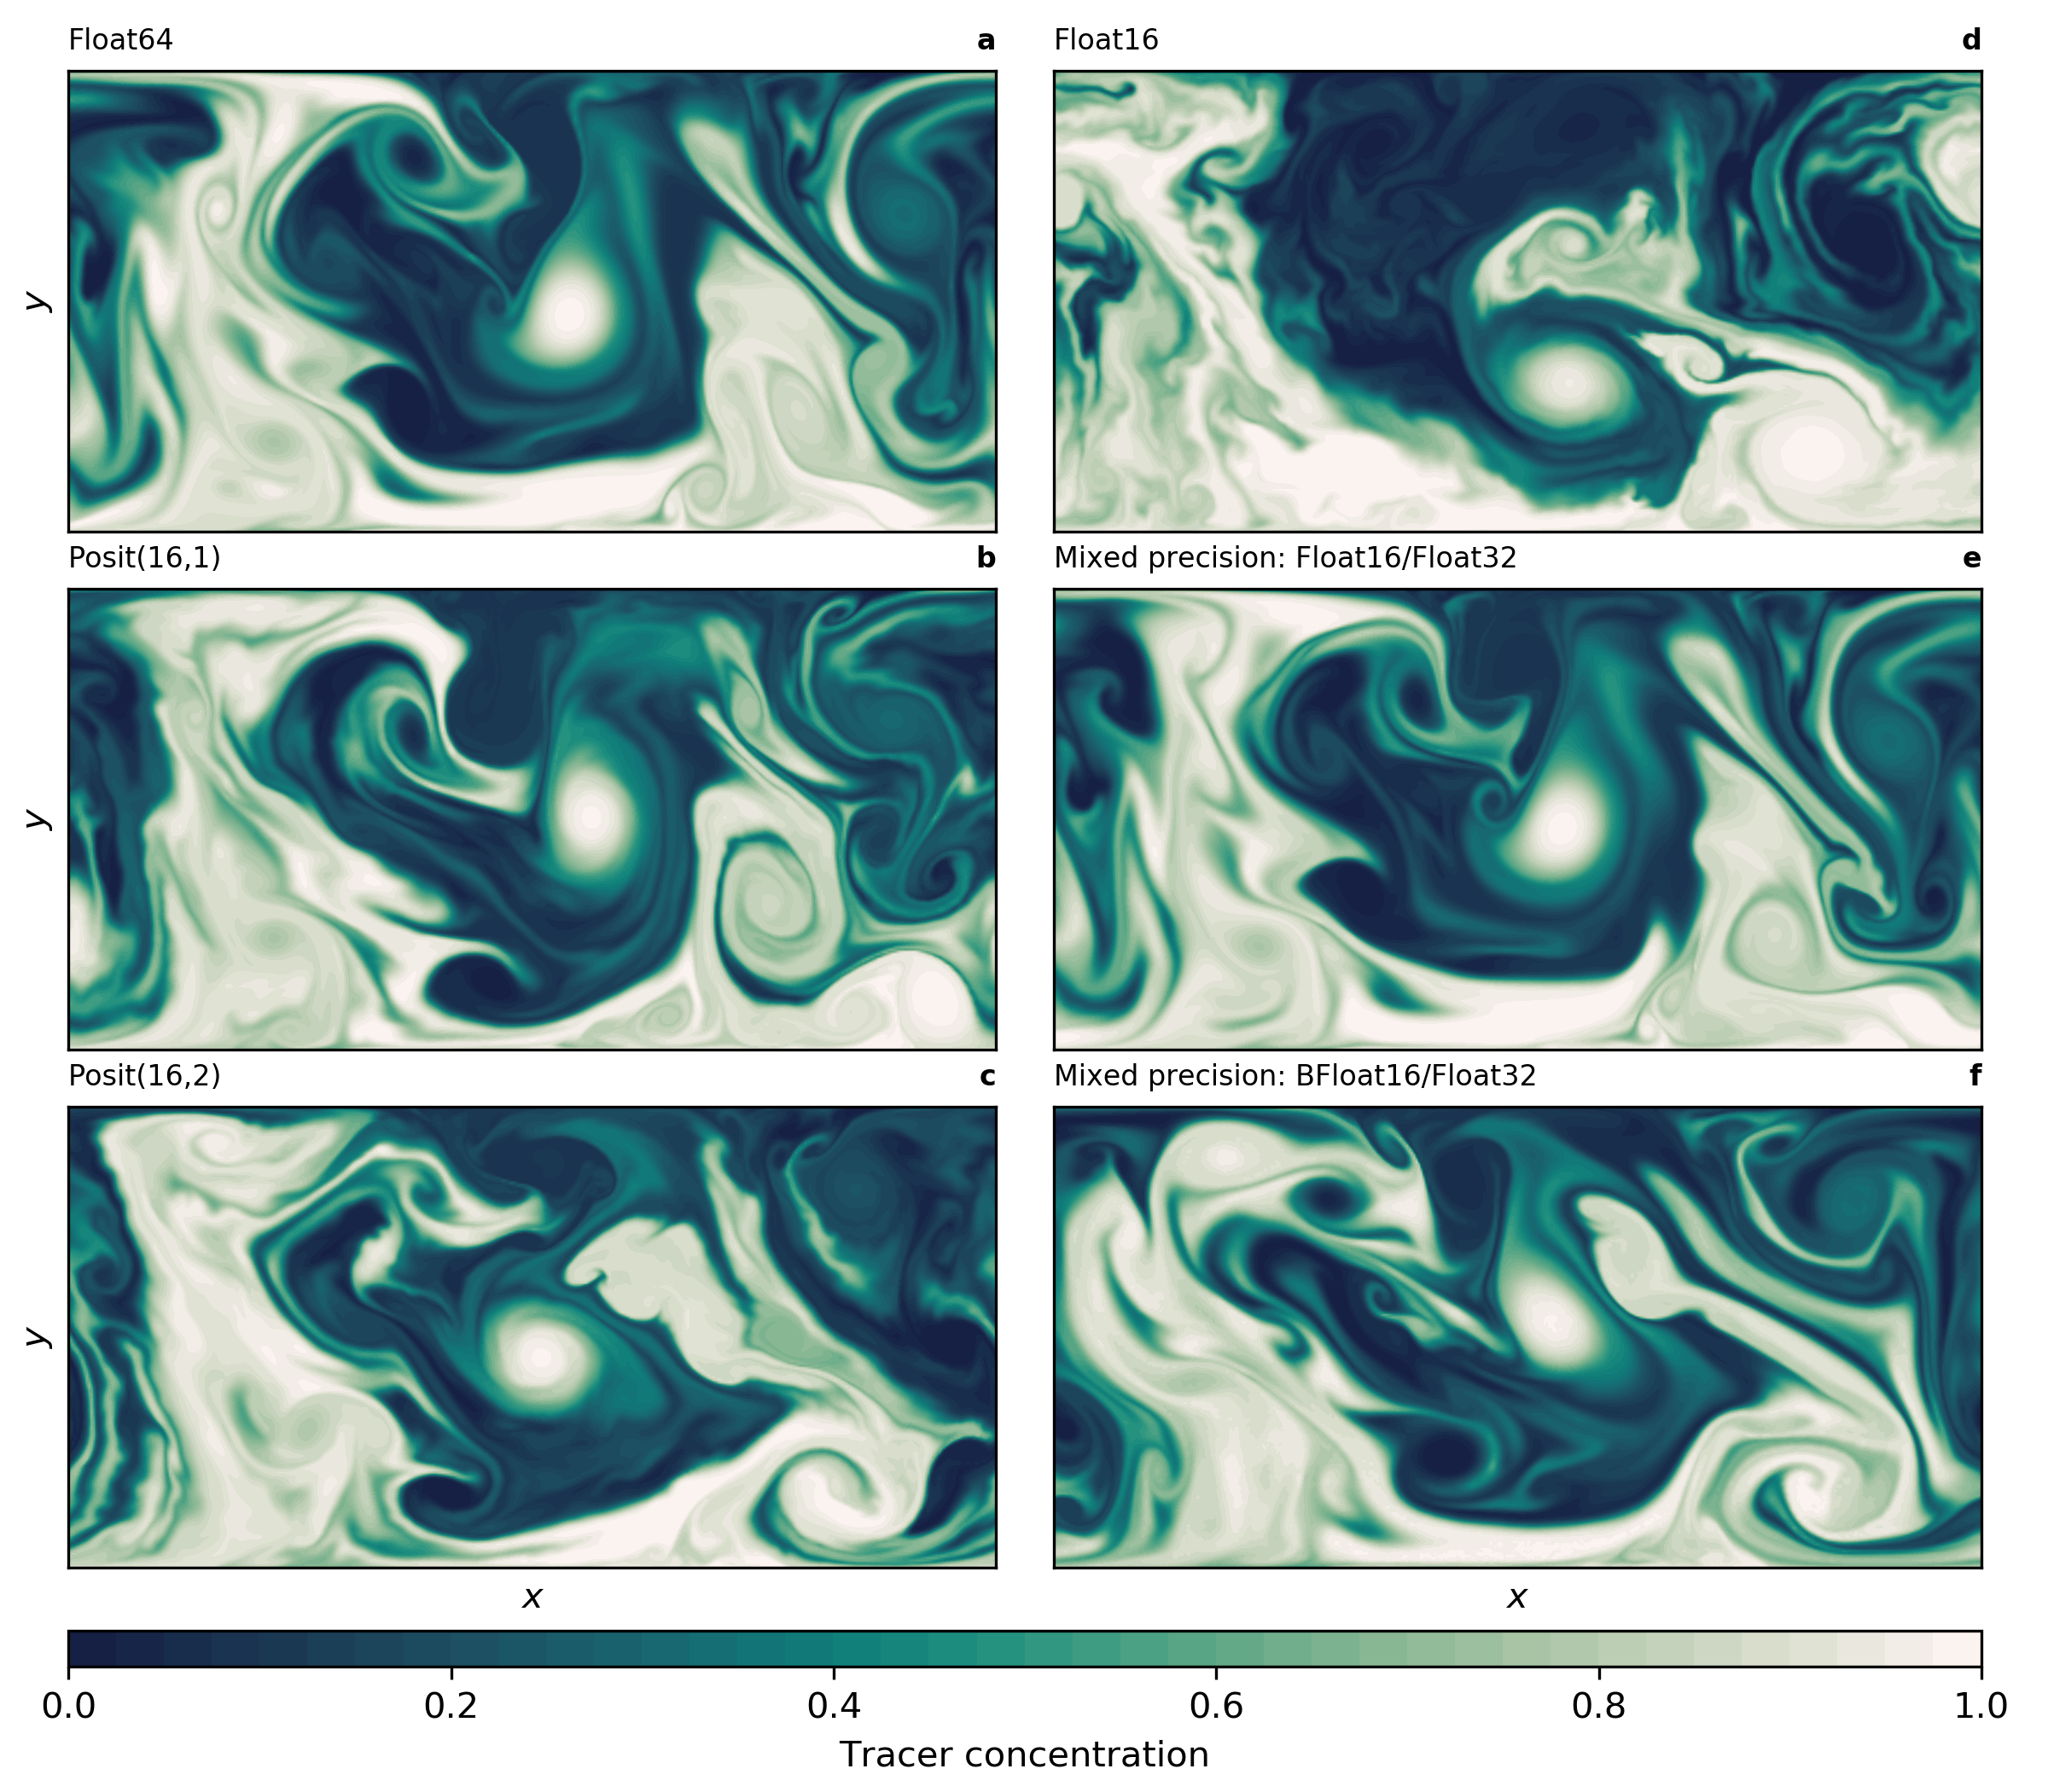
\includegraphics[width=1\textwidth]{Figures/swm/snapshot.png}
\caption{Snapshot of tracer concentration simulated by the shallow water model
using different 16-bit number formats and the high-resolution configuration
($\Delta = 5$km). The mixed precision simulations presented in (e) and (f) are
using Float32 for the representation of prognostic variables only. The tracer
was injected uniformly in the lower half of the domain 50 simulation days before
the time step shown.}
\label{fig:snapshot}
\end{figure}

The shallow water model simulates vigorous turbulence interacting with a
zonal current (Fig. \ref{fig:snapshot}). Both float and posit arithmetic
present very similar fluid dynamics in comparison to the Float64 reference in
only 16 bit. A snapshot of tracer concentration many simulated days after
initialisation reveals turbulent mixing of the tracer that is well simulated
with posits. However, with Float16 the simulation deviates faster from the
reference than with Posit(16,1) and to a lesser degree with Posit(16,2),
presumably due to the small scale instabilities visible in the snapshot as
wavy filaments and fronts. These instabilities are clearly triggered by Float16
arithmetics, but to a lower degree also visible for posits. This provides some
visual evidence that accumulated rounding errors are reduced with posits, especially
Posit(16,1). BFloat16 arithmetic is not able to simulate the shallow water dynamics,
as tendencies are too small to be added to the prognostic variables. A stalling
of the simulated flow is observed. The results with mixed precision,
Float16/Float32 and BFloat16/Float32, will be discussed in section 3.3.

\begin{figure}
\includegraphics[width=1\textwidth]{Figures/swm/rmse_eta_darker.pdf}
\caption{Forecast error of sea surface height $\eta$ measured as root mean square
error (RMSE) taking Float64 as reference. (a) Forecast error for various 16-bit
number formats and mixed 16/32-bit simulations for which the prognostic variables
are kept in Float32. (b) Forecast error for reduced precision communication in
8 or 16 bit with various number formats used for encoding, with Float64 used for
all calculations. The communication of boundary values occurs at every time step
for the prognostic variables. The RMSE is normalised by a mean forecast error at
very long lead times. Solid lines represent the median of 200 forecasts per number
format. The shaded areas of each model configuration denote the interquartile
range of the forecast experiments.}
\label{fig:rmse}
\end{figure}

Short-term forecasts at medium-resolution ($\Delta = 10$km) are performed to
analyse the differences between different 16-bit arithmetics. To quantify the error
growth caused by rounding errors with different arithmetics in a statistically
robust way, we create a number of forecasts with each member starting from one
of 200 randomly picked start dates from a 50-year long control simulation. The
forecast error in the shallow water model is computed as root mean square error
(RMSE) of sea surface height $\eta$ with respect to Float64 simulations. Other
variables yield similar results. Each forecast is performed several times from
identical initial conditions but with the various number formats. The error growth
caused by rounding errors is additionally compared to the error
introduced by discretisation. A low-resolution model configuration with
$\Delta = 20$km is used to quantify a realistic level of discretisation error.
The RMSE is normalised by the climatological mean forecast error at very long lead
times, which is the same for all model configurations. When the normalised RMSE
reaches 1 all information on the initial conditions is removed by the chaotic
evolution of the shallow water system.

The forecast error of Float16 is as large as the discretisation error and
clearly outperformed by 16-bit posit arithmetic (Fig. \ref{fig:rmse}a).
Both Posit(16,1) and Posit(16,2) yield a forecast error that is several times
smaller than Float16. The forecast error of 32-bit arithmetic is several orders
of magnitude smaller and is only after 200 days as large as the error for 16-bit
arithmetic at short lead times of about 10 days. Also at 32 bit, posits clearly
outperform floats.

\begin{figure}
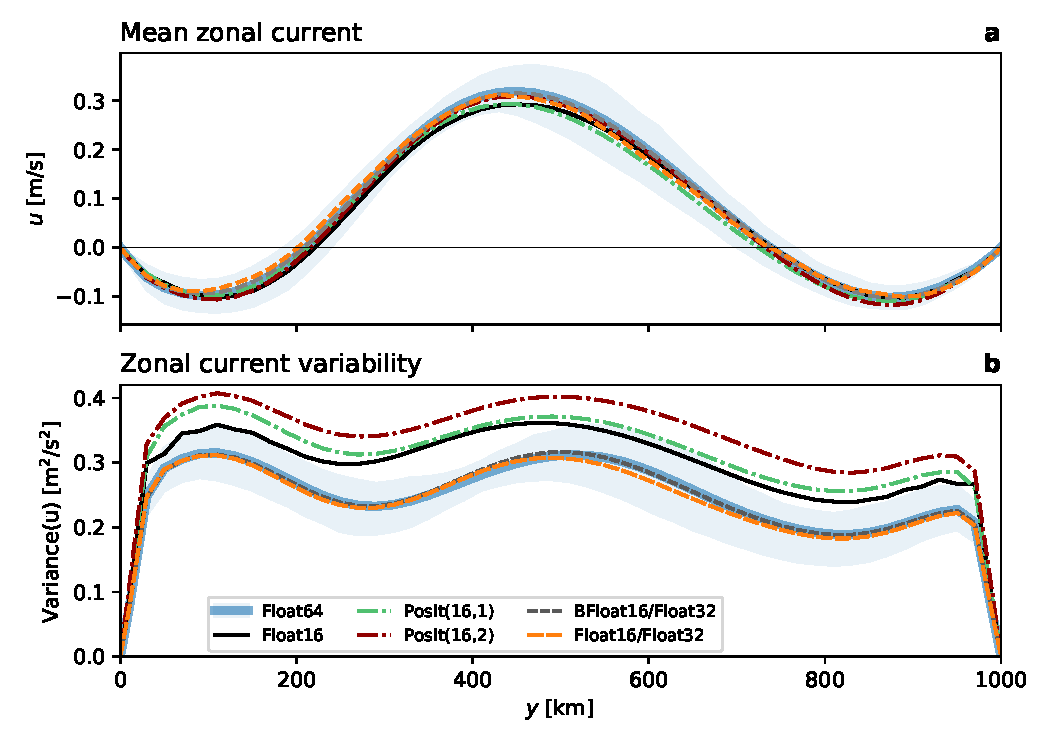
\includegraphics[width=1\textwidth]{Figures/swm/meanvar_u.pdf}
\caption{Climatology and variability of the zonal current in the medium-resolution
simulations. (a) Zonally-averaged zonal current $u$ as a function of the meridional
coordinate $y$. (b) Zonal variance of the zonal current as a function of $y$.
The dashed lines for BFloat16/Float32 and Float16/Float32 are almost identical.
The shaded area denotes the interquartile temporal variability around the (a) mean and
(b) variance of reference simulation with Float64.}
\label{fig:mean}
\end{figure}

To investigate the effect of rounding errors on the climatological mean state of
the shallow water system, we zonally average the zonal velocity $u$. This average
is based on 300-day long simulations starting from 200 different initial conditions,
which cover the various states in the long-term variability of the shallow water system.
However, the climatology from a single very long simulation has not been assessed.

The mean state is an eastward flow of about 0.3~m/s, about 3 to 4 times weaker than
individual velocities throughout the domain (Fig. \ref{fig:mean}a), which is typical
for turbulent flows. A weak westward mean flow is found at the northern and
southern boundary. No 16-bit format was found to have a significant impact on
the mean state. The variability of the flow around its mean state is high
throughout the domain (Fig. \ref{fig:mean}b). The variability is significantly
increased by 10 -- 30\% with 16-bit arithmetic, especially with Posit(16,2).
This is probably caused by rounding errors that are triggering local
perturbations which increase variability.

\begin{figure}
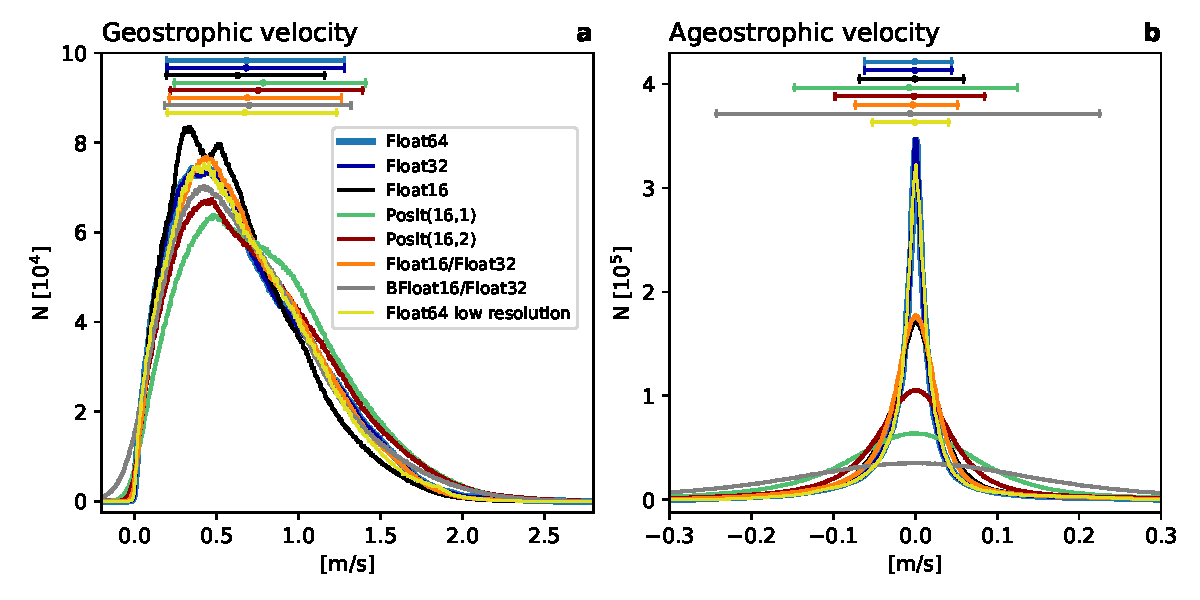
\includegraphics[width=1\textwidth]{Figures/swm/ageostrophic.pdf}
\caption{Geostrophic balance as simulated with different number formats.
(a) Histograms of flow-parallel components of geostrophic velocity.
(b) as (a) but for the ageostrophic velocities. Horizontal bars denote the
mean, 10th and 90th-percentile in respective colours.}
\label{fig:geo}
\end{figure}

The turbulence in shallow water simulations is largely geostrophic, such that the
pressure gradient force opposes the Coriolis force. The resulting geostrophic
velocities $\mathbf{u}_g$ can be derived from the sea surface height $\eta$ as
\begin{subequations}
\begin{align}
\mathbf{u}_g &= \frac{g}{f}\hat{\mathbf{z}} \times \nabla \eta \\
\mathbf{u} &= \mathbf{u}_{g} + \mathbf{u}_{ag}
\end{align}
\label{eq:geo}%
\end{subequations}
and deviations from the actual flow $\mathbf{u}$ are the ageostrophic velocity
components $\mathbf{u}_{ag}$. We project both components on the actual velocities
to obtain the flow-parallel components $\tilde{u}_{g}$ and $\tilde{u}_{ag}$ via
\begin{equation}
\tilde{u}_g = \frac{\mathbf{u}_g \cdot \mathbf{u}}{\| \mathbf{u} \|},
\quad \tilde{u}_{ag} = \frac{\mathbf{u}_{ag} \cdot \mathbf{u}}{\| \mathbf{u} \|}.
\label{eq:parallel}%
\end{equation}
The geostrophic velocities in the shallow water simulations can reach up to 2 m/s,
are hardly negative (i.e. against the flow) and have a mean of about 0.7 m/s
(Fig. \ref{fig:geo}a). This behaviour is well simulated with 16-bit number formats,
although posits increase the strength of geostrophic velocities slightly. Ageostrophic
velocity components are found to be isotropic, and are oriented equally frequent
with and against the prevailing flow. They rarely exceed $\pm$0.1m/s and are
therefore comparably small, which is expected in geostrophically balanced turbulence.
Ageostrophic velocities can be seen as a measure of the physical instabilities in
the flow field and their variance is indeed increased when simulated with
16-bit number formats. Float16 and posits show clearly fewer ageostrophic velocities
around 0, pointing towards an increased number of simulated instabilities.
Especially Posit(16,1) increases the variance of ageostrophic velocities by more
than a factor of two. It is unclear where in the model integration rounding errors
of 16-bit arithmetic trigger instabilities that lead to the observed increase in
ageostrophy. We conclude that although the geostrophic balance in the simulations
is maintained, rounding errors lead, likely due to an increase in ageostrophy,
to a higher variability in the flow field.

\begin{figure}
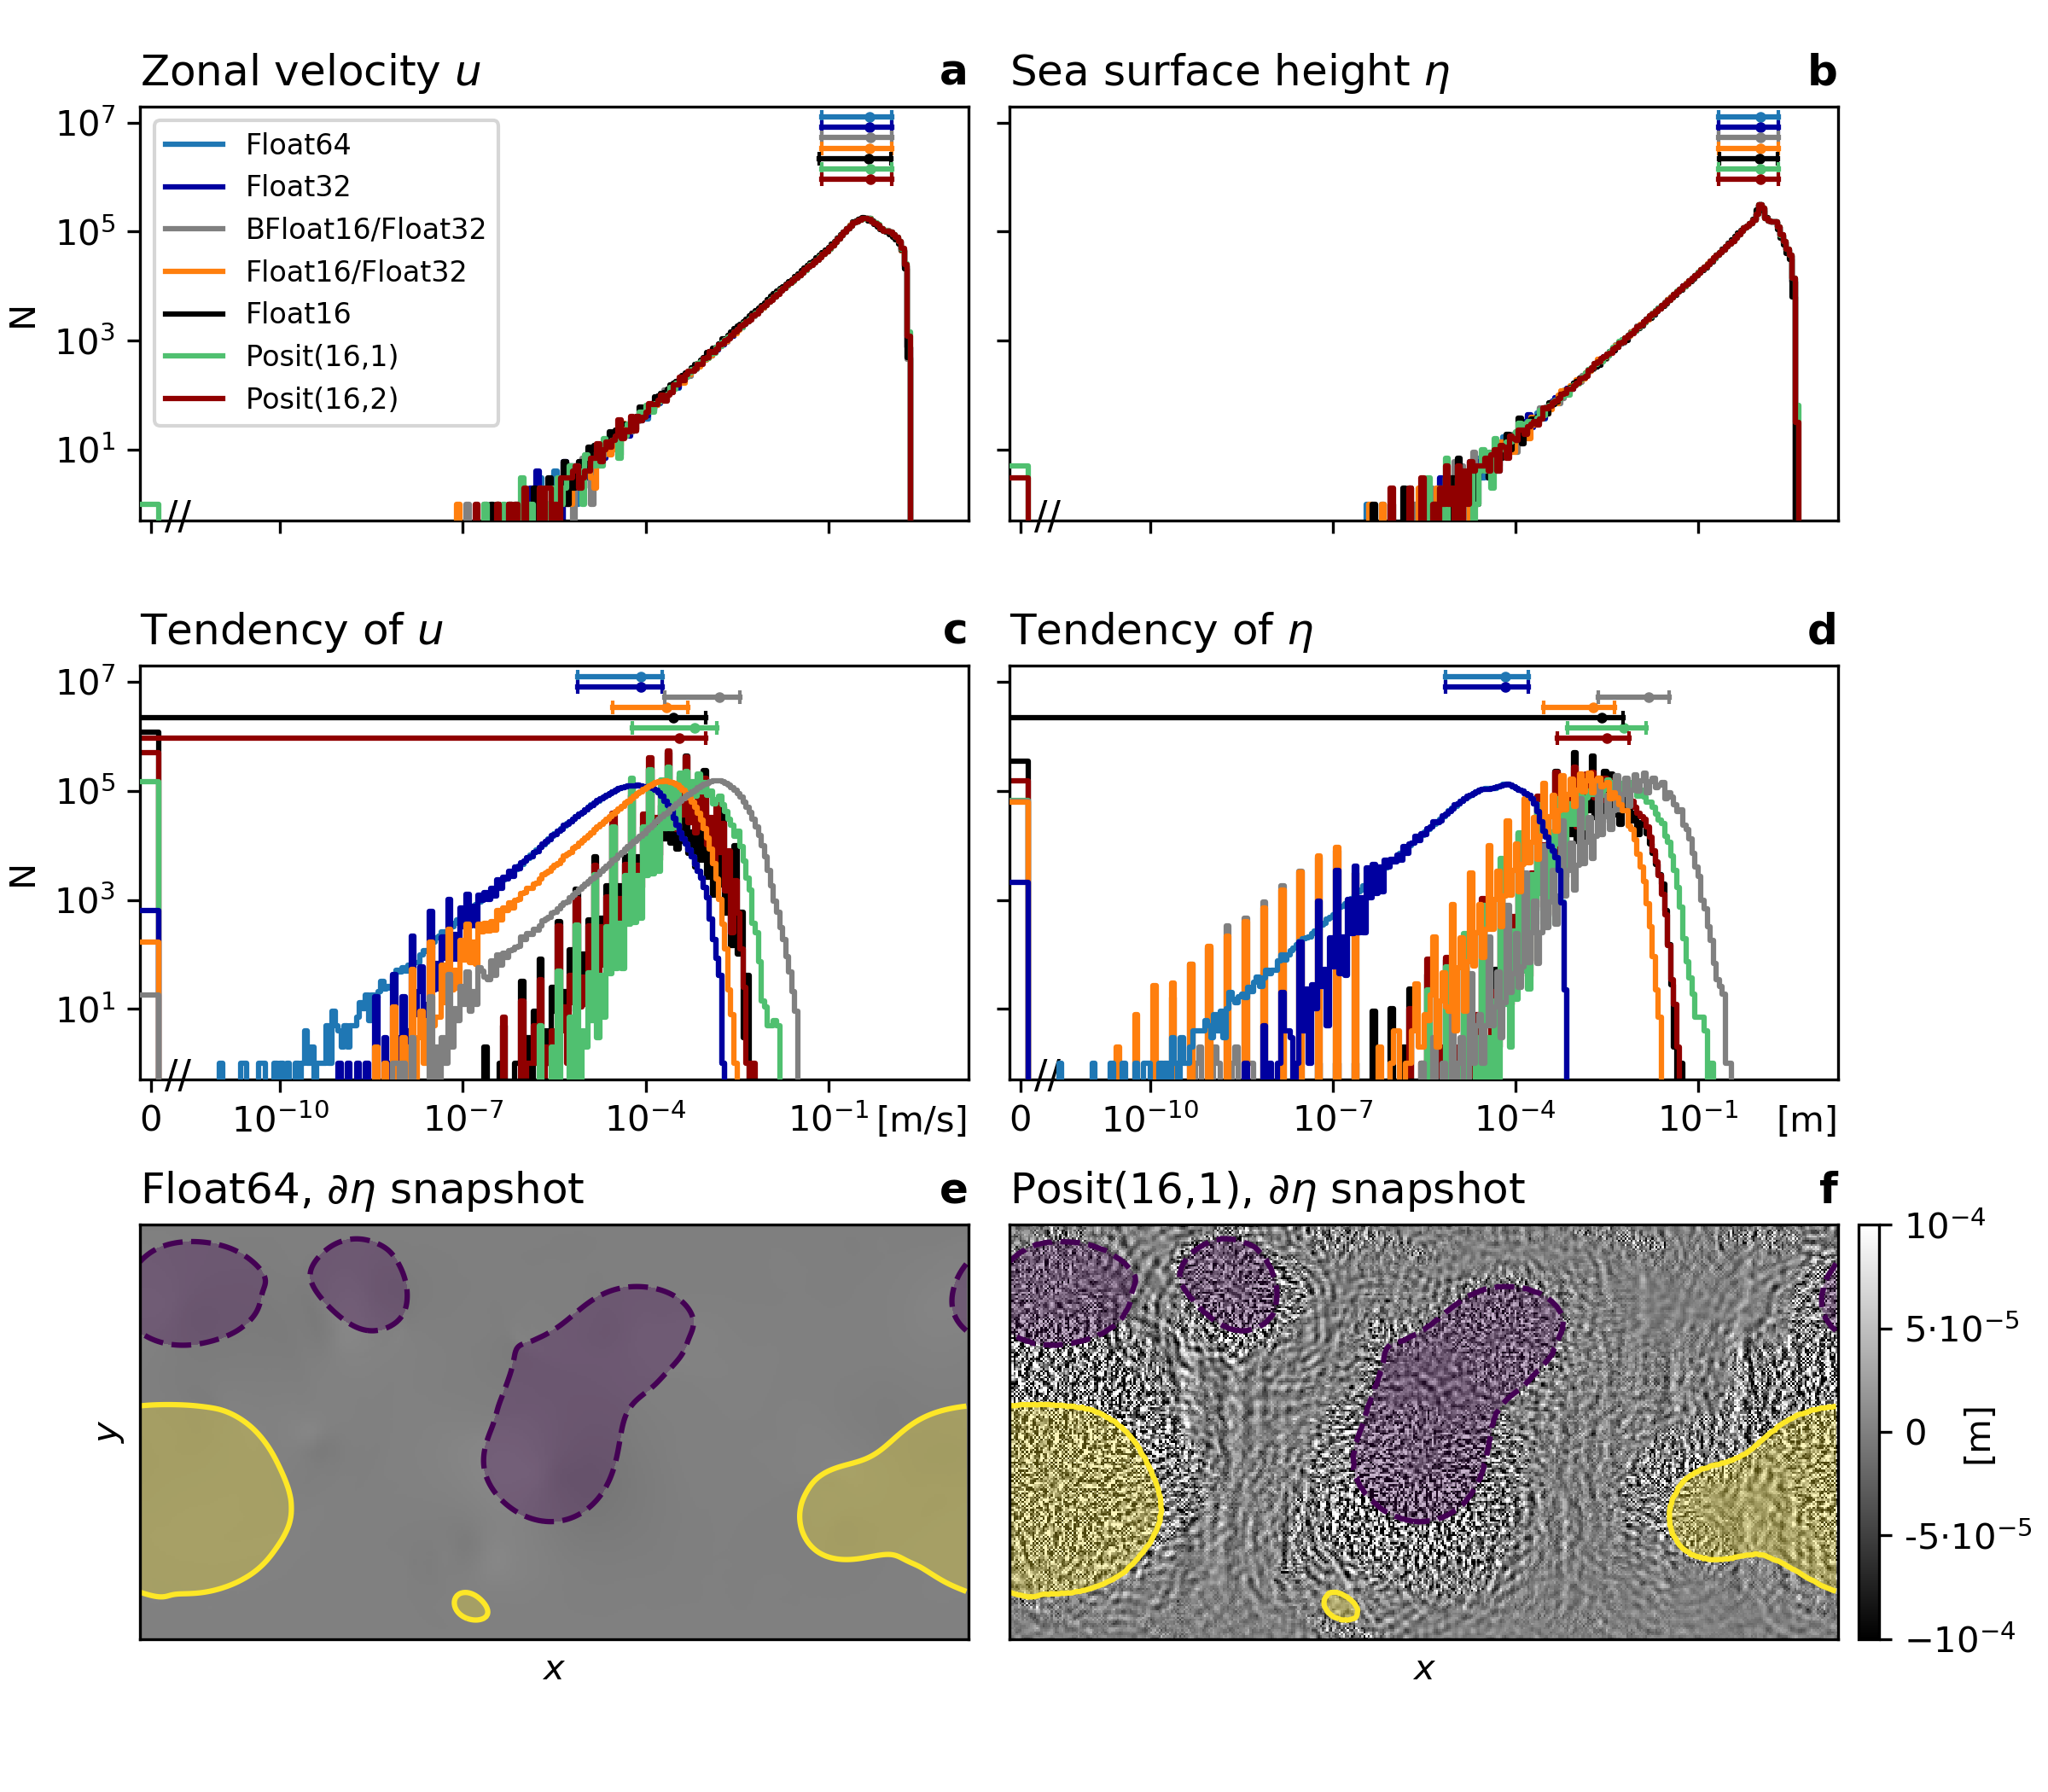
\includegraphics[width=1\textwidth]{Figures/swm/tendency_hist2.png}
\caption{Histograms of the numeric values of the prognostic variables (a) zonal
velocity $u$, (b) sea surface height $\eta$, and the respective tendencies of
(c) $u$ and (d) $\eta$, simulated with different 16, 32
and 64-bit number formats. Mean, 10th and 90th percentile are shown above the
histograms in respective colors. Snapshots of the tendencies of $\eta$ simulated
with (e) Float64 and (f) Posit(16,1). Snapshots are similar for other 16-bit formats
(not shown here). Areas of sea surface height anomalies exceeding $\pm1.4$~m are
shown in purple (negative) and
yellow (positive). Note the break on the x-axis close to zero in (a,b,d) and (e).}
\label{fig:tend}
\end{figure}

As 16-bit arithmetics have no significant impact on the climatological mean state,
histograms of prognostic variables are also not changed (Fig. \ref{fig:tend}a and b).
However, the tendencies are increased by orders of magnitude with 16-bit arithmetics
(Fig. \ref{fig:tend}d and e), as rounding errors cause gravity waves to radiate
away from eddies (Fig. \ref{fig:tend}f). Gravity waves are identified from the
tendency of sea surface height. Comparing their propagation to the location of
anomalous sea surface height, which is used as a proxy to locate eddies, we
assume that rounding errors in regions of high eddy activity lead to instabilities
that propagate away in the form of gravity waves. These gravity waves are not
present in Float64 simulations (Fig. \ref{fig:tend}c) and tend to have only a
small impact on quasi-geostrophic dynamics, as they act on different time and
length scales. It is unclear but possible that gravity waves cause the observed
increased ageostrophic velocities for 16-bit arithmetic.

Tendencies are about 4 orders of magnitude smaller than the prognostic variables.
This poses a problem for number formats with a machine epsilon, measured as decimal
precision, significantly lower than 4 decimal places (Table \ref{tab:formats}).
Float16 has a machine epsilon of 3.7, which is presumably close to the lower limit
beyond which the addition of tendencies will be round back. The BFloat16 number
format has a machine epsilon of 2.8, which explains why flow is stalling when
simulated with BFloat16.

In the previous simulations the entire shallow water simulation was performed
with the specified number format. As the addition of tendencies to the prognostic
variables was identified as a key calculation that is error-prone, we investigate
now the benefits of mixed precision arithmetic, where Float32 is used for the
prognostic variables but the tendencies are computed with either Float16 or
BFloat16, two number formats that have the lowest decimal precision around 1.
The prognostic variables are now reduced to Float16 or BFloat16 before calculations
of the right-hand side and every term of the tendencies is converted back before
addition to the prognostic variables. Using subscripts 16 and 32 to denote variables
held at 16 and 32-bit precision, respectively, and let Float32() be the conversion
function. The continuity equation (Eq. \ref{eq:swe}b) then becomes
\begin{equation}
\frac{\partial \eta_{32}}{\partial t} = -\op{Float32}( \partial_x(u_{16}h_{16})
+ \partial_y(v_{16}h_{16} ))
\label{eq:conversion}
\end{equation}
and similar for $u$ and $v$ in Eq. \ref{eq:swe}a.

Snapshots of tracer concentration reveal well simulated geostrophic turbulence
(Fig. \ref{fig:snapshot}e and f) with Float16/Float32 or BFloat16/Float32 and
instabilities at fronts or in filaments are visibly reduced compared to pure
16-bit arithmetic. The forecast error is strongly reduced once the prognostic
variables are kept as Float32 (Fig. \ref{fig:rmse}a), supporting the hypothesis
that the addition of tendencies to the prognostic variables is a key computation
with low rounding error-tolerance. Despite BFloat16 not being suitable for shallow
water simulations when applied to all computations, mixing BFloat16 with Float32
arithmetic yields a similar error growth to posits, which is well below the
discretization error. Mean state or variability are virtually identical for both
mixed precision cases (Fig. \ref{fig:mean}) compared to the Float64 reference.
The geostrophic balance is largely unaffected, but ageostrophic velocities increase
in variance, especially for BFloat16 (Fig. \ref{fig:geo}). Gravity waves are
similarly present for mixed precision although weaker for tendencies computed
with Float16 (Fig. \ref{fig:tend}d) and, as discussed, they tend to not interact
with the geostrophic time and length scales. Although the results show that Float16
is generally a preferable number format over BFloat16 for the applications presented
here, we acknowledge that the conversion between Float32 and Float16 will come
with some computational cost. In contrast, the conversion between BFloat16 and
Float32 is computationally very cheap as both formats have the same number of
exponent bits. Removing significant bits, applying rounding, and padding
trailing zeros, are the only operations for this conversion. Following the
results here, mixing 16 and 32-bit precision is found to be an attractive solution
to circumvent spurious behaviour due to 16-bit floating-point arithmetics.
Performance benefits are still possible as most calculations are performed with
16 bit, with error-critical computations in 32 bit to reduce the overall error.

Using mixed-precision in our shallow water model, 77\% of the arithmetic
operations are performed in 16 bit and the remaining 23\% in 32 bit. Assuming
Float16/BFloat16 to be two times faster than Float32 and conversion costs to
be negligible this would yield another 40\% reduction in computing time on top
of a reduction from Float64 to Float32. However, this depends on the soft
and hardware implementation considered. Some of the 16-bit accelerators (GPU/TPU)
can increase the flop rate by more than a factor of 2 when compared to Float32.
In addition, the shallow water model regarded here has a comparably simple
right-hand side, such that more complex models will spend more time to compute
tendencies which will come with a larger performance increase.

Mixed-precision is an attractive solution as hardware-accelerated 16-bit
floating-point arithmetic is already available on graphic or tensor processing
units and implementations therefore do not rely on the development of future
computing hardware, which is the case for posits.

\begin{figure}
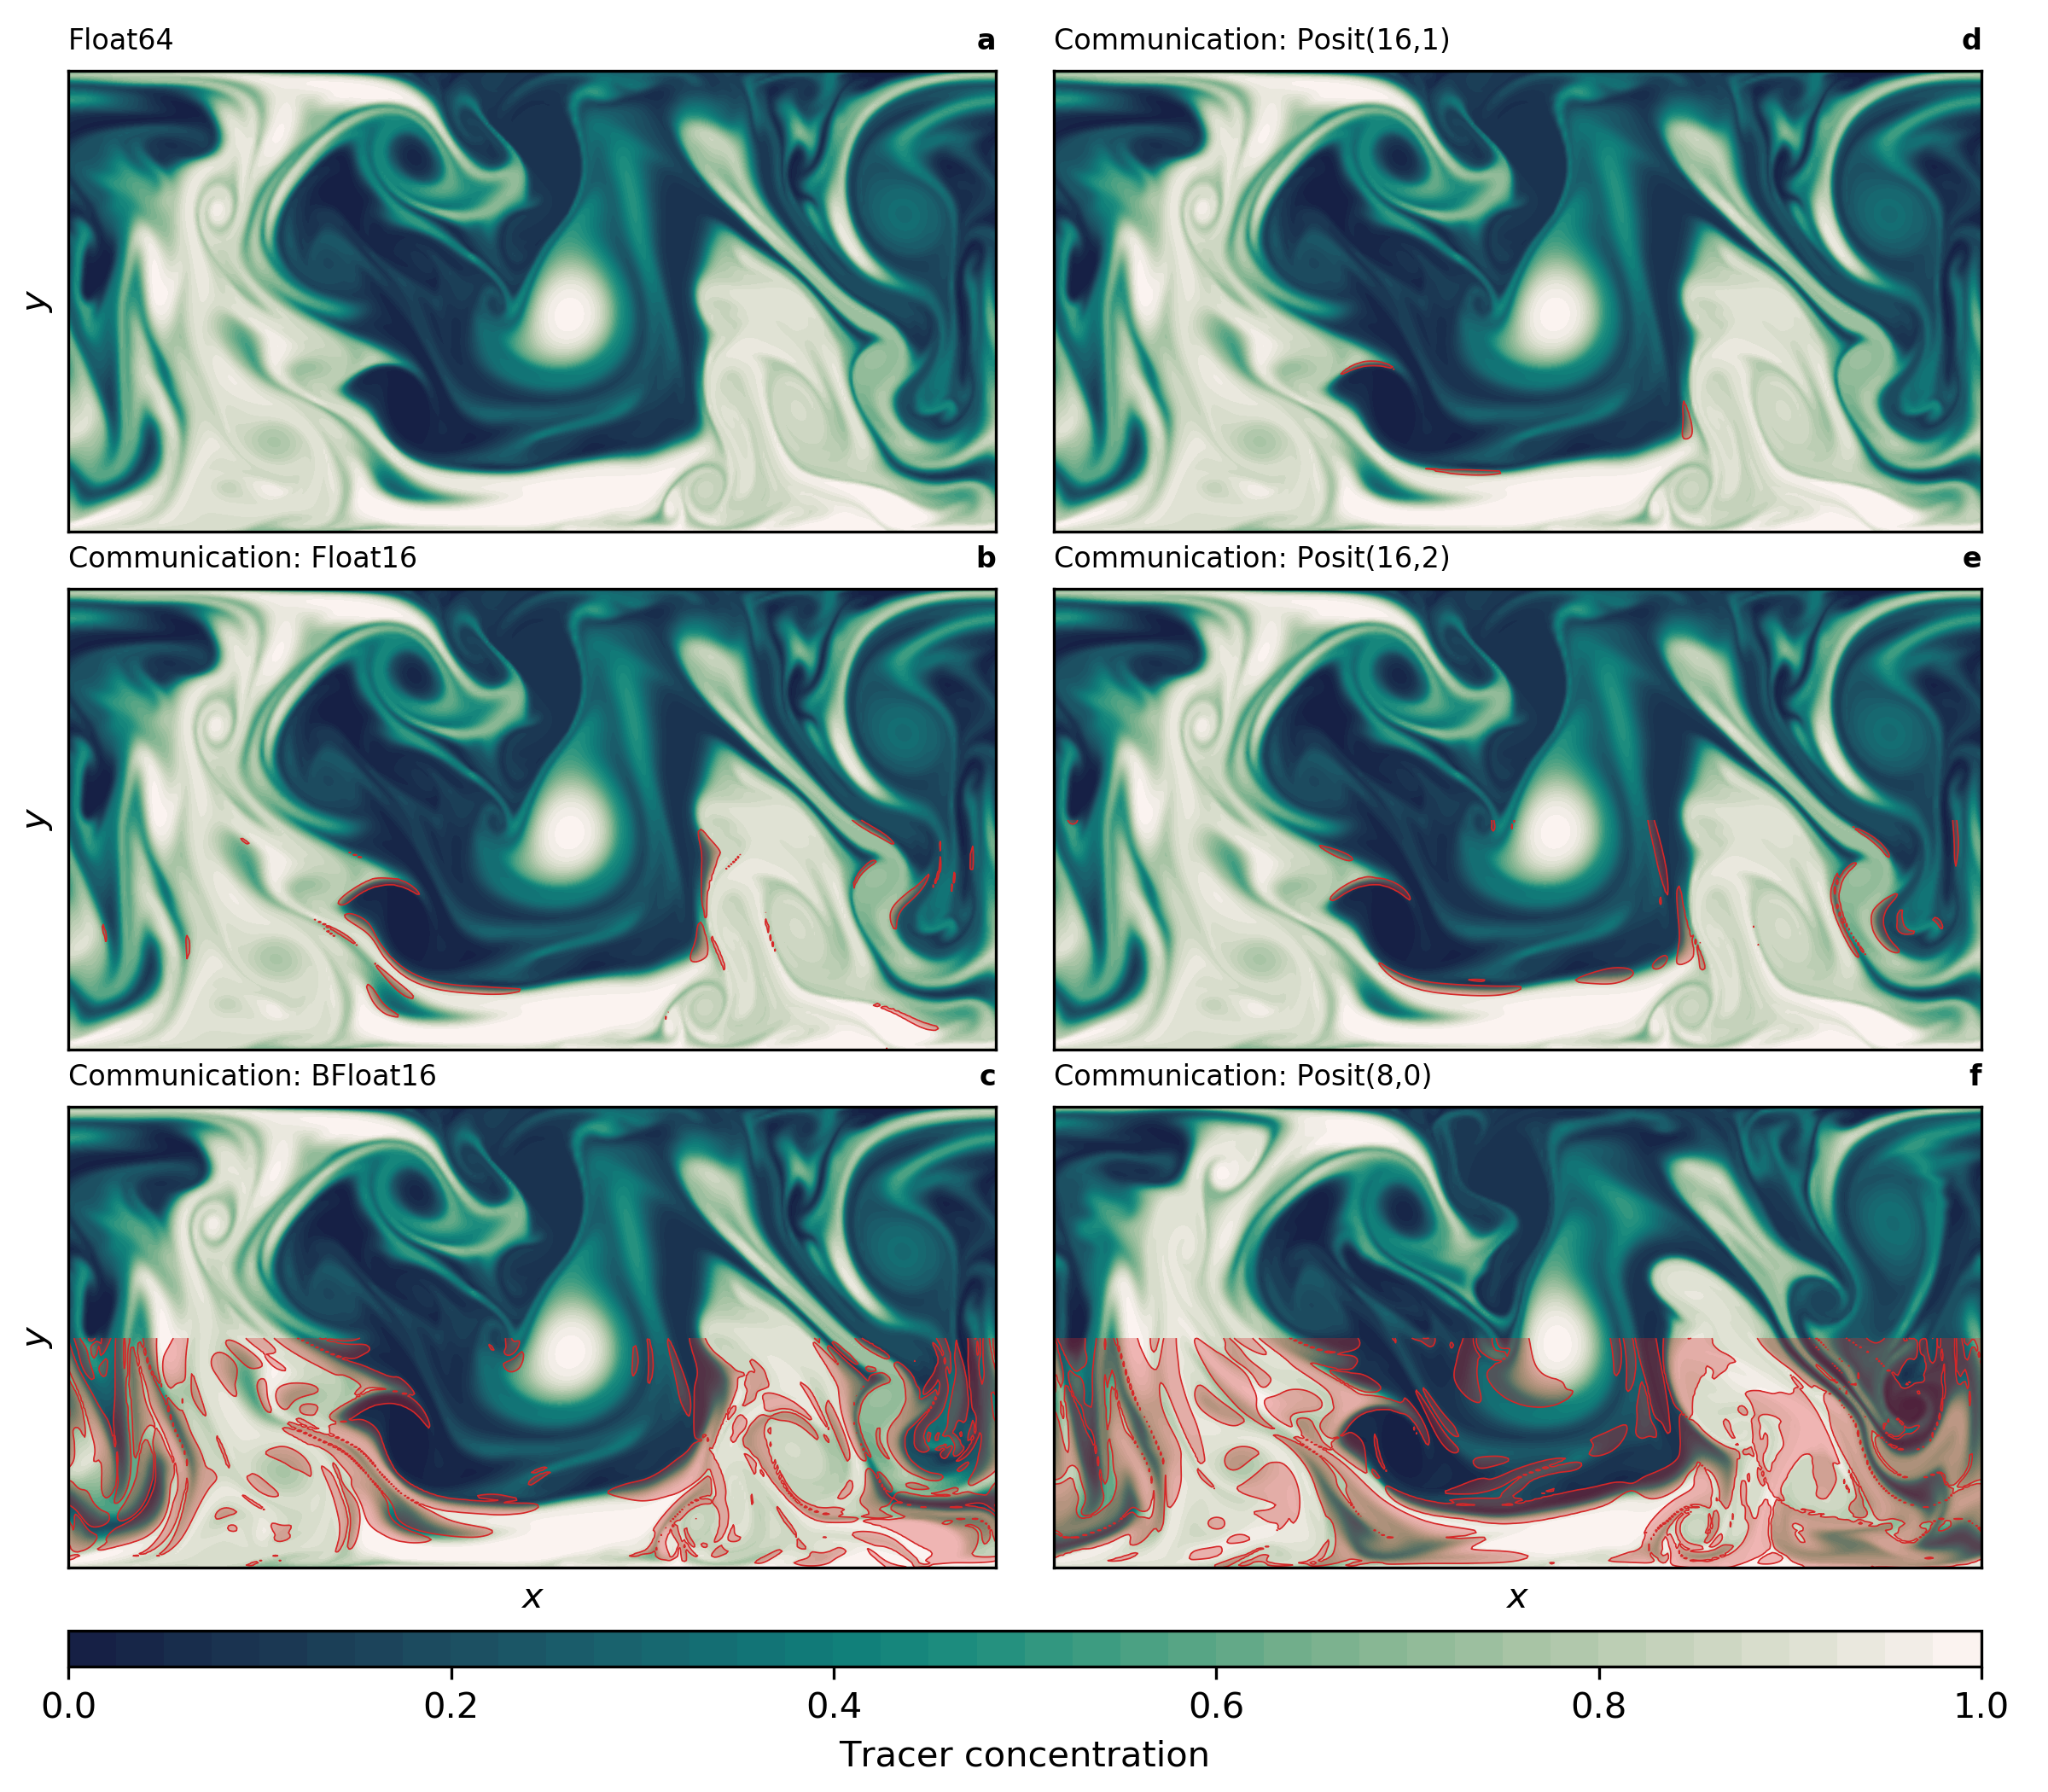
\includegraphics[width=1\textwidth]{Figures/swm/snapshot_comm.png}
\caption{Snapshot of tracer concentration simulated by the shallow water model
using reduced precision communication. The communication of boundary values occurs
at every time step for the prognostic variables. Float64 was used for all calculations.
Areas where the absolute error exceeds 0.05 are shaded in red only in the lower
half of the domain. The tracer was injected uniformly in the lower half of the
domain 50 days before. This simulation was run in the high-resolution
configuration ($\Delta = 5$km).}
\label{fig:snapshot_comm}
\end{figure}

A standard method to parallelise simulations is the distributed-memory parallelism
via Message Passing Interface (MPI). We emulate MPI-like communication in the
shallow water model with the copying of boundary values between the right and
left boundary (periodic boundary conditions). Although the shallow water model
does not run in parallel, reducing the precision in the copying of boundary values
introduces an equivalent error as if reduced precision MPI communication was used
between subdomains. Reduced precision is applied for the communication of the
prognostic variables at every Runge-Kutta substep.

Regarding snapshots of tracer concentration simulated with reduced precision
communication shows a negligible error for Float16 and posits (Fig. \ref{fig:snapshot_comm}).
The error is largest at fronts and not concentrated around the boundaries.
Encoding the communication with BFloat16 introduces a larger error than for the
other 16-bit formats as the decimal precision is with 2.8 clearly lower
(Table \ref{tab:formats}) for the range of values occurring within the prognostic
variables (Fig. \ref{fig:tend}a and b). The errors are quantified by the RMSE of
surface height $\eta$ as before and are up to about two orders of magnitude smaller
than the errors that result from 16-bit arithmetic. As even the worst 16-bit
communication format, BFloat16, has a smaller error than the best mixed precision
formats, Float16 with Float32, we extend the short-term forecast experiments to
include two 8-bit formats, Posit(8,0) and Float8 (see Table \ref{tab:formats} for
a description). Both formats are found to be suitable for reduced precision
communication here and do not introduce an error that is larger than the
discretization error. Having said that, Float8 communication introduces an error
that is comparably large in the first days but growths only linearly in the first
50 days of the simulation, which is in contrast to the exponential error growth
observed for 16-bit arithmetic.

\subsection{Error growth}
\subsection{Mean and variability}
\subsection{Geostrophy}
\subsection{Gravity waves}
\subsection{Mass and tracer conservation}

\section{Discussion}
Future high performance computing architecture will support some 16-bit
arithmetics. The wall-clock time for weather and climate simulations could
be greatly reduced if computationally demanding algorithms were run at such
reduced precision. We tested a number of options for 16-bit arithmetic for
weather and climate applications in a shallow water model. The best results
were achieved with 16-bit posits (with either 1 or 2 exponent bits) which appear
very promising for application in high performance computing for Earth System
modelling. Float16 can be used to perform forecasts with the shallow water model
while the application of BFloat16 or integer arithmetic was not successful.

In general, 16-bit arithmetics were not found to alter the climatological mean
state or the large-scale dynamics. However, variability and ageostrophic velocities
were increased, such that second and higher-order statistics should undergo
testing to assess the models reliability. Depending on the application, an increased
variability does not necessarily deteriorate the model, especially for more
realistic model set-ups than considered here. However, our findings suggest that
reduced precision changes need to be done carefully as specific simulation features
can change without obvious impact on mean diagnostics.

Shallow water simulations with 16-bit arithmetic required rescaling of some terms
but no major revisions of the model code or algorithms. Given that only floats are
currently hardware-supported, we investigated mixed precision approaches.
Keeping the prognostic variables at 32 bit while computing the tendencies in 16 bit
reduced the rounding errors significantly. We also showed that numerical precision
for communication between compute nodes can be greatly reduced down to 16 or
even 8-bit without introducing a large error. Reduced precision communication was
not found to have a significant impact on either mean state, variability,
geostrophy or tendencies.

A \emph{perfect model} is used in this study, such that any form
of model or initial condition error is ignored and only the number format is
changed between simulations. Solely discretisation errors are estimated by
lowering the spatial resolution by a factor of 2. Although this is essential
here to analyse the impact of rounding errors isolated from other errors, it
is in general not a realistic configuration for weather or climate models. More
complex models include many other sources of forecast error, such that the
contribution of rounding errors from 16-bit arithmetic would likely be dwarfed by
model, discretisation or initial condition errors.

Only the most common discretisation method for fluid dynamics was used in
this study: Finite differences with an explicit time stepping scheme. But various
other discretisation methods exist, such as finite element or volume, spectral
methods and implicit time stepping. These methods come with different algorithms
and associated precision requirements. Consequently, some might be
less tolerant to rounding errors than the method used in this study.

There is currently no hardware available for posit arithmetic that we could have used
for performance testing and it is seems impossible to make credible estimates
whether such hardware would be faster or slower when compared to hardware
optimised for Float16 arithmetic (as this does not only depend on theoretical
considerations but also on investments into chip design). We therefore cannot
draw any conclusion about the performance of posit arithmetic operations in
comparison to Float16 or the other formats.

Until progress is made on hardware implementations for posits, the results here
suggest that also 16-bit float arithmetic can successfully be used for parts of
complex weather and climate models with the potential for acceleration on graphic
and tensor processing units. It is therefore recommended to adapt a type-flexible
programming paradigm, ideally in a language that supports portability, with
algorithms written to reduce the dynamic range of arithmetic results. Hardware
progress on central, graphic or tensor processing units, with various numbers
formats supported, can subsequently be utilised to accelerate weather and
climate simulations.

\chapter{Running on 16-bit hardware}
\label{chap:hardware}

%% CONTRIBUTION
\small
\paragraph{Contributions} This chapter is largely based on the following publication\footnote{with the following author contributions.
Conceptualisation: MK, SH, MC. Data curation: MK. Formal Analysis: MK. Methodology: MK. Visualisation: MK. Writing – original draft:
MK. Writing – review \& editing: MK, SH, MC, PDD, TNP.}

\vspace{\baselineskip}
\indent M Klöwer, S Hatfield, M Croci, PD Düben and TN Palmer, 2021. \emph{Fluid simulations accelerated with 16 bit:
Approaching 4x speedup on A64FX by squeezing ShallowWaters.jl into Float16}, \textbf{Journal of Advances in Modeling
Earth Systems}, in review. Preprint \href{https://doi.org/10.1002/essoar.10507472.2}{10.1002/essoar.10507472.2}
\vspace{\baselineskip}
\hrule
\vspace{\baselineskip}
\normalsize

\paragraph{Abstract.} Most Earth-system simulations run on conventional CPUs in 64-bit double-precision floating-point numbers
Float64, although the need for high-precision calculations in the presence of large uncertainties has been questioned. Fugaku,
currently the world’s fastest supercomputer, is based on A64FX microprocessors, which also support the 16-bit low-precision format
Float16. We investigate the Float16 performance on A64FX with ShallowWaters.jl, the first fluid circulation model that runs entirely
with 16-bit arithmetic. The model implements techniques that address precision and dynamic range issues in 16 bit. The precision-critical
time integration is augmented to include compensated summation to minimize rounding errors. Such a compensated time integration is
as precise but faster than mixed precision with 16 and 32-bit floats. As subnormals are inefficiently supported on A64FX the very
limited range available in Float16 is $6 \cdot 10^{-5}$ to $65504$. We develop the analysis-number format Sherlogs.jl to log the arithmetic results
during the simulation. The equations in ShallowWaters.jl are then systematically rescaled to fit into Float16, using 97\% of the available
representable numbers. Consequently, we benchmark speedups of 3.8x on A64FX with Float16. Adding a compensated time integration
the speedup is 3.6x. Although ShallowWaters.jl is simplified compared to large Earth-system models, it shares essential algorithms and
therefore shows that 16-bit calculations are indeed a competitive way to accelerate Earth-system simulations on available hardware.


\section{Introduction}

The first numerical weather prediction models have recently moved away from 64-bit double-precision floating-point numbers
for higher computational efficiency in lower precision \citep{Govett2017,Nakano2018,Rudisuhli2013,Vana2017}. While both Float32
and Float64 formats are widely available for high-performance computing, support for 16-bit arithmetic is only available on mainstream
hardware for a few years, due to the demand for low precision by the deep learning community. The transition towards 16 bit is challenging
for an existing application: Rounding errors from low precision have to be controlled and a limited range of representable numbers
cannot be exceeded without causing often catastrophic under and overflows. But the potential performance gains are promising,
with 4x speedups compared to 64-bit calculations, not to mention the reduced energy consumption.

The current boom in machine learning applications is supported by advances in microprocessors. Instead of conventional central
processing units (CPU), graphic and tensor processing units GPU, TPU \citep{Jouppi2018,Jouppi2018a,Jouppi2017,Steinkraus2005}
are used, which are better suited for the workloads of machine learning. While most supercomputers from \href{https://top500.org}{TOP500.org}
are based on Intel CPUs with the x86-64 architecture \citep{Dongarra2011}, many new installations transition towards GPUs or alternative
microprocessor architectures \citep{Zheng2020}. The trend is towards heterogeneous computing with specialised hardware, which is
both a challenge and an opportunity for weather and climate models \citep{Bauer2021,Bauer2021a}. Fugaku, the world’s fastest supercomputer
as of 2020, is based on Fujitsu’s A64FX processors with ARM architecture \citep{Odajima2020,Sato2020}. The A64FX also implements the
Float16 format (1 sign, 5 exponent and 10 mantissa bits) and Fujitsu promises a 4x increase in the number of floating-point
operations per second. 

Float16 is the 16-bit variant of Float32 and Float64 and is defined in the 2008 revision of the IEEE-754 standard on floating-point arithmetic
\citep{IEEE1985,IEEE2008}. Alternatives such as BFloat16 \citep{Burgess2019, Kalamkar2019}, minifloats \citep{Fox2020}, logarithmic
fixed-point numbers \citep{Johnson2020,Johnson2018,Sun2020}, posits
\citep{Gustafson2017a,Chaurasiya2018,Klower2019a,Klower2020a,Langroudi2019,Zhang2020} and stochastic rounding
\citep{Croci2020,Hopkins2020,Mikaitis2020,Paxton2021} have been investigated, but most of these are not available on
standard supercomputing hardware. Currently only floats (and integers) enjoy a widely available support in terms of hardware,
libraries and compilers that ultimately make it possible to execute complex computational applications.

The use of low-precision number formats is motivated as in the presence of large uncertainties in the climate system rounding
errors are masked by other sources of error \citep{Palmer2015}. Typical rounding errors from high-precision calculations are
many orders of magnitude smaller than errors in the observations, from coarse resolution or underrepresented physical processes.
Low-precision calculations are therefore, at least in theory, sufficient without a loss in accuracy for a weather forecast or a climate prediction.
Emulated in parts of weather and climate models, 16-bit half precision has been shown to be a potential route to accelerated simulations
\citep{Dawson2018,Chantry2019, Hatfield2019, Klower2020a}.

Although weather and climate model data often comes with large uncertainties, many intermediate calculations inside a model simulation
require a higher precision. Time integration is often a precision-critical part of numerical simulations of dynamical systems. Stability constraints
require small time steps such that tendencies are often several times smaller than the prognostic variables \citep{Courant1967}.
Adding the two yields a loss of precision from the tendency as small increments can only be poorly resolved in low precision
\citep{Gill1951,Kahan1965,Moller1965}. In extreme cases this can lead to a model stagnation \citep{Croci2020}, and is often
dealt with using mixed-precision approaches \citep{Dawson2018,Klower2020a,TintoPrims2019}, where the tendencies are computed
in low precision, but converted to a high-precision format before addition. This is beneficial as a large share of computing time is
accelerated with low precision, while precision-critical operations are kept in high precision.

Precision loss in calculations can be analysed with a variety of available tools, like FPBench \citep{Damouche2017},
CADNA \citep{Jezequel2008}, Verrou \citep{Fevotte2019}, and Verificarlo \citep{Denis2016}. Such tools are often either
based on interval arithmetic, providing rigid rounding error bounds, or on stochastic arithmetic to assess the rounding error growth.
While these can be useful to identify the minimal decimal precision for simulating chaotic systems, analysing the limited dynamic range
of low-precision number formats is largely unaddressed in these tools.

In this chapter, we present, to our knowledge, the first modern fluid circulation model that runs entirely in hardware-accelerated 16-bit floats on the
ARM architecture-based microprocessor A64FX. Strategies are presented to solve precision and range issues with 16-bit arithmetic:
In section \ref{sec:hardware_methods} we scale the shallow water equations, and an appropriate scale is found with the
newly-developed analysis-number format Sherlogs.jl. Additionally, a compensated time integration is presented to minimise
precision issues. Section \ref{sec:hardware_speedup} analyses the rounding errors of Float16 in ShallowWaters.jl and
benchmarks the performance compared to Float64. Section \ref{sec:hardware_discussion} discusses the results.

\begin{figure}[tbhp]
	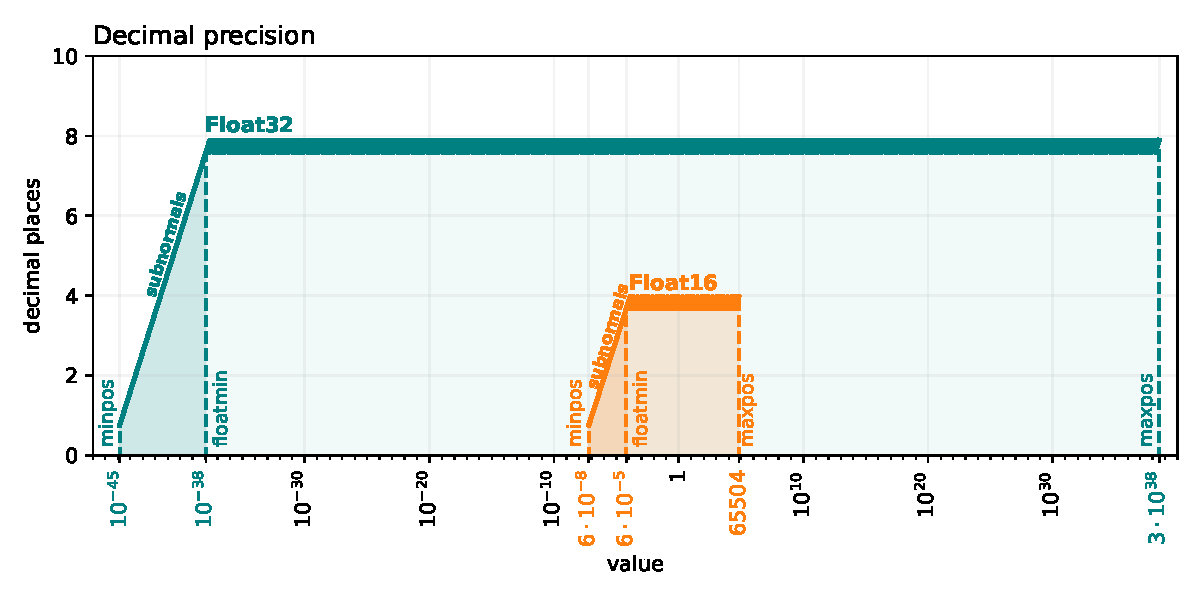
\includegraphics[width=1\textwidth]{Figures/a64fx/float32_16_decprec.pdf}
	\caption{\textbf{Decimal precision of Float16 and Float32 over the range of representable numbers.}
	The decimal precision is worst-case, i.e. given in terms of decimal places that are at least correct after rounding (see section
	\ref{sec:decimal_precision}). The smallest representable number ($minpos$, see section \ref{sec:floats}), the smallest normal
	number ($floatmin$) and the largest representable number ($maxpos$) are denoted with vertical dashed lines. The subnormal
	range is between $minpos$ and $floatmin$.}
	\label{fig:a64fx_decprec}
\end{figure}

\section{Methods}
\label{sec:hardware_methods}

 The following methods describe in section \ref{sec:swm_scaling} the scaling of the shallow water equations, which is extended from 
 the dimensionless gradients introduced in section \ref{sec:swm_scale}. The shallow water model presented here is an updated
 version from the one presented in chapter \ref{chap:shallow_water}. Section \ref{sec:scale_sherlogs} describes how to choose a scale
 guided by an analysis number format, a concept introduced in section \ref{sec:analysis_number_formats}. To reduce rounding errors
 in the time integration we describe the compensated time integration in section \ref{sec:compensated_time_integration}.

\subsection{Scaling the shallow water equations}
\label{sec:swm_scaling}

The shallow water equations describe an oceanic flow idealised to two horizontal dimensions. They result from
a vertical integration of the Navier-Stokes equations \citep{Gill1982,Vallis2006} after several approximations.
The shallow water equations are simplified but representative of many weather and climate models, which are
usually solved with many vertically-coupled horizontal layers. They describe the time
evolution of the prognostic variables velocity $\mathbf{u} = (u,v)$, and interface height $\eta$  in the following form 
\begin{align}
\partial_t\mathbf{u} &+ \mathbf{u} \cdot \nabla \mathbf{u} + f\mathbf{z} \times \mathbf{u} =
-g\nabla \eta + \nu_B \nabla^4 \mathbf{u} - r \mathbf{u} + \mathbf{F}, \nonumber \\
\partial_t\eta &+ \nabla \cdot (\mathbf{u}h) = 0 \nonumber \\ 
\partial_tq &+ \mathbf{u} \cdot \nabla q = -\tau(q-q_0),
\label{eq:swm_a64fx}
\end{align}
The shallow water model and its discretisation is explained in more detail in Appendix \ref{sec:swm_appendix}. Here we
discuss the parameter choices relevant for this chapter and in contrast to the previous chapter which used an older version
of the same model. The shallow water equations are defined over a rectangular domain
with zonal and meridional coordinates $x,y$ of size $L_x = 8000\op{km}$, $L_y  = 4000\op{km}$, respectively. The domain
is a zonal channel with boundary conditions being periodic in $x$. The channel setup is motivated by zonal oceanic flows like
the Antarctic Circumpolar Current but highly idealised \citep{Jansen2015,Jansen2015a}.

In contrast to the barotropic model setup in chapter \ref{chap:shallow_water}, we reduce the gravitational acceleration to
$g = 0.1\op{ms}^{-2}$. A reduced gravity is usually chosen to represent baroclinic dynamics in a two-layer ocean
with a rigid surface and an interface $\eta$ between them. The lower layer is motionless. Despite its physical representation,
here the main motivation to reduce gravity is to slow down gravity waves which allows for longer time steps.
The shallow water gravity wave speed is with $c_{ph} = 7 \mathrm{ms}^{-1}$ a factor of 10 slower than in
chapter \ref{chap:shallow_water}, which allows for 10 times longer time steps.

The Rossby number $Ro$ is small for basin-wide motions, $Ro < 0.01$, but unity is approached for dynamics near the grid scale,
which is here on the order of kilometres. The Coriolis parameter changes from $f=7\cdot10^{-5}~\mathrm{s}^{-1}$ at the southern boundary
to $f=1.4\cdot10^{-4}~\mathrm{s}^{-1}$ at the northern boundary. The Rossby radius of deformation $L_R = \tfrac{c_{ph}}{f}$ is
between 50 and 100~km and in comparison to chapter \ref{chap:shallow_water} smaller due to slower gravity waves.

To increase the turbulence throughout the domain, the zonal wind forcing $\mathbf{F} = (F_x,0)$ is a meridional shear
$F_x = F_0\sin(\omega t) \tanh(2\pi(yL_y^{-1} - \tfrac{1}{2}))$ which reverses seasonally ($\omega^{-1} = 365\op{days}$). 
In comparison to chapter \ref{chap:shallow_water} this effectively reduces the spin-up time, requiring fewer computational
resources at higher resolution. Similarly, four meridional ridges on the seafloor have been added, irregularly spaced in the zonal direction,
in comparison to chapter \ref{chap:shallow_water} to trigger more instabilities in the zonal flow. All mountain ridges have
a height of $H_1 = 100~\mathrm{m}$ compared to the fluid depth of $H_0 = 500~\mathrm{m}$.

To better visualise the turbulence throughout the domain, the advection for the passive tracer $q$ (Eq. \ref{eq:swm_a64fx})c)
includes a relaxation term, which slowly restores the tracer field to the reference $q_0$ at the time scale of $\tau^{-1} = 100\op{days}$.
Bottom friction is disabled in simulations in this chapter ($c_D = 0$ in Eq. \ref{eq:diss}), but for illustrative purposes we retain
a linear bottom friction term $-r\mathbf{u}$ in the scaling of the shallow water equations. 

In order to control the range of numbers occurring in the simulation, the shallow water equations are scaled with a multiplicative
constant. The evaluation of linear terms is not affected, but the non-linear terms involve an unscaling. The same constant $s$
is chosen for zonal velocity $u$  and meridional velocity $v$, such that $\hat{u} = su$ and $\hat{v} = sv$.
Additionally, we use dimensionless spatial gradients $\hat{\partial_x} = \Delta x \partial_x, \hat{\nabla} = \Delta x \nabla$, etc.
by scaling the equations with the grid spacing $\Delta x$. For simplicity, we use the same $\Delta x$ in $x$ and $y$-direction
but generalisation to less regular grids is possible. The grid spacing $\Delta x$ is then combined with the time step
$\widehat{\Delta t} = \tfrac{\Delta t}{\Delta x}$ and $\hat{\partial_t} = \Delta x \partial_t$. Due to the 4th-order gradient in the
viscosity, we scale its coefficient as $\hat{\nu_B} = \Delta x^{-3}\nu_B$. Using the potential vorticity $h^{-1}(f + \zeta)$,
with the relative vorticity $\zeta = \partial_xv - \partial_yu$, and the Bernoulli potential $\tfrac{1}{2}(u^2 + v^2) + g\eta$,
the shallow water equations can be written into a vector-invariant form (section \ref{sec:vector_invariant}). A scaled version
of this form is solved by the numerical model and reads as
\begin{align}
\hat{\partial_t}\hat{u} &= \frac{[s\Delta x f]+ \hat{\zeta}}{\hat{h}}\frac{\hat{v}\hat{h}}{s} -\hat{\partial_x}
\left([\frac{1}{2s}](\hat{u}^2 + \hat{v}^2) + [\frac{sg}{s_\eta}]\hat{\eta} \right) + \hat{\nu_B} \hat{\nabla}^4 \hat{u}
- [r\Delta x]\hat{u} + [s\Delta x F_x], \nonumber \\
\hat{\partial_t}\hat{v} &= - \frac{[s\Delta x f]+ \hat{\zeta}}{\hat{h}}\frac{\hat{u}\hat{h}}{s} -\hat{\partial_y}
\left([\frac{1}{2s}](\hat{u}^2 + \hat{v}^2) + [\frac{sg}{s_\eta}]\hat{\eta} \right) + \hat{\nu_B} \hat{\nabla}^4 \hat{v}
- [r\Delta x]\hat{v} + [s\Delta x F_y].
\end{align}
Square brackets denote pre-computed constants and only the volume fluxes $uh,vh$ have to be unscaled on every time step.
As the volume fluxes are quadratic terms, the evaluation of $\hat{u}\hat{h}$ scales as $s^2$, which therefore has to be
partly unscaled with $s^{-1}$. The continuity equation is rescaled with $s_\eta$, i.e. $\hat{\eta} = s_\eta \eta$ as well as
$\hat{h} = \hat{\eta} + s_\eta H$, and the tracer advection equation is rescaled with $s_q$, so that $\hat{q} = s_q q$.
\begin{align}
\hat{\partial_t} \hat{\eta} &= -\hat{\partial_x}(\frac{\hat{u}\hat{h}}{s}) - \hat{\partial_y}(\frac{\hat{v}\hat{h}}{s}), \nonumber \\
[s\hat{\partial_t}] \hat{q} &= \left(-\hat{u}\hat{\partial_x} \hat{q} - \hat{v}\hat{\partial_y} \hat{q}\right) - [\tau \Delta x](\hat{q} - \hat{q_0}).
\end{align}
ShallowWaters.jl solves these scaled shallow water equations with 2nd order finite differencing on a regular,
but staggered Arakawa C-grid \citep{Arakawa1977}. The advection of potential vorticity uses the energy
and enstrophy-conserving scheme of \cite{Arakawa1990}. The tracer advection equation for $q$ is solved
with a semi-Lagrangian advection scheme \citep{Diamantakis2013,Smolarkiewicz1992}. This scheme calculates
a departure point for every arrival grid point one time step ago. The tracer field is then interpolated onto the departure point,
which is used as the tracer concentration at the arrival point for the next time step. More details on the implementation of
the semi-Lagrangian advection scheme is described in section \ref{sec:swm_semilagrange}. The time integration of
ShallowWaters.jl is discussed in section \ref{sec:compensated_time_integration}.

\subsection{Choosing a scale with Sherlogs}
\label{sec:scale_sherlogs}

The scaling of equations has to be implemented carefully when using number formats with a limited dynamic range,
such as Float16 (Fig. \ref{fig:a64fx_decprec}). Subnormals for Float16 are in the range of $6 \cdot 10^{-8}$ to
$6 \cdot 10^{-5}$ (see section \ref{sec:floats}) and are inefficiently supported on some hardware, such that their occurrence
causes large performance penalties. This reduces the available range of Float16 even further and a simulation
has to fit as best as possible in the remaining 9 orders of magnitude between $6.104 \cdot 10^{-5}$ and $65504$.
A single overflow, i.e. a result above $65504$, will abort the simulation. Understanding the range of numbers
that occur in all operations and ideally in which lines of the code is therefore very important. 
For most algorithms this is very difficult to achieve unless the numbers are directly measured within the simulation. 

\begin{figure}[tbhp]
\begin{lstlisting}[language=JuliaLocal, label=lst:sherlogs, caption={\textbf{Example usage and output of Sherlogs.jl,
a package for Sherlogs and DrWatson, two analysis-number formats that can be combined with type-flexible
functions in Julia.} Using Sherlog16 as the first argument of \texttt{run\_model} runs ShallowWaters.jl with Float16 but
also logs the bitpattern of every arithmetic result into a \emph{logbook} of length $2^{16}=65536$ to create a bitpattern
histogram. \texttt{DrWatson16\{f\}} uses Float16 but also records a stack trace (a list of calling functions and respective
lines of code) every time the function \texttt{f(x)} evaluates to \texttt{true} with the arithmetic result \texttt{x}.
Here, a subnormal arises in a multiplication ($*$ in line 14 here) in line 320 of the code in script \texttt{time\_integration.jl.}}]
julia> using ShallowWaters, Sherlogs       # load packages
julia> # run ShallowWaters with Sherlog16 which logs all arithmetic results
julia> run_model(Sherlog16)                # use Sherlog16 as number format

julia> get_logbook()                       # retrieve the bitpattern histogram
65536-element LogBook(1112720887, 1484631, 1378491, 1024411, ... , 0, 0, 0)

julia> # run ShallowWaters with DrWatson16 recording a stack trace when f=true
julia> f(x) = 0 < abs(x) < floatmin(Float16)  # true for subnormals
julia> run_model(DrWatson16{f})            # use DrWatson16 as number format

julia> get_stacktrace(1)                   # retrieve the first stack trace
3-element Vector{Base.StackTraces.StackFrame}:
* at DrWatson16.jl:52 [inlined]            # subnormal occurred in *
caxb!(...) at time_integration.jl:320      # inside this function
time_integration(...) at time_integration.jl:82 # called from here
\end{lstlisting}
\end{figure}

We therefore developed the analysis number format Sherlogs. See section \ref{sec:analysis_number_formats} for a general
description of code composability and analysis number formats. Sherlog16, for example, uses Float16 to compute,
but after every arithmetic operation the result is also logged into a bitpattern histogram. Running a simulation with
Sherlogs will take considerably longer due to the overhead from logging the arithmetic results, which can be obtained
in the form of a bitpattern histogram upon completion. The bitpattern histogram will reveal information such as the
smallest and largest occurring numbers or how well an algorithm fits into a smaller dynamic range.
An example usage of Sherlogs is given in Listing \ref{lst:sherlogs}.

Sherlogs are implemented in the package Sherlogs.jl, which makes use of the type-flexible
programming paradigm in Julia \citep{Bezanson2017}. A function is written in an abstract form,
which is then dynamically dispatched to the number format provided and compiled just-in-time.
Such a number format can therefore be, for example, Float64 or Float16, but also any user-defined
number format such as Sherlogs.

An appropriate scaling $s,s_\eta,s_q$ has to be chosen for a given set of parameters. The bitpattern
histogram of the entirely unscaled shallow water equations simulated with Float32 reveals range issues
that would arise with Float16 (Fig. \ref{fig:a64fx_bitpatternhist}a). A large share (10\%) of the arithmetic
results would be below the representable range of Float16. Consequently, running the model without
any scaling modifications in Float16 would round many numbers to 0, causing so-called underflows
that deteriorate the simulated dynamics \citep{Klower2020a}. Most of these underflows occur in the
calculation of gradients, which consequently have to be non-dimensionalised as previously suggested
\citep{Klower2019a}. This also largely removes a resolution-dependence of the bitpattern histograms,
such that Float16 simulations are possible across a wide range of resolutions. Dimensionless gradients
are a major improvement to fit ShallowWaters.jl into the available range with Float16, yet 3\% of the
arithmetic results are subnormals (Fig. \ref{fig:a64fx_bitpatternhist}b). On A64FX a flag can be set to
avoid the performance penalty from subnormals by flushing every occurring subnormal to zero.
The smallest representable number is therefore $6.104 \cdot 10^{-5}$.

\begin{figure}[tbhp]
	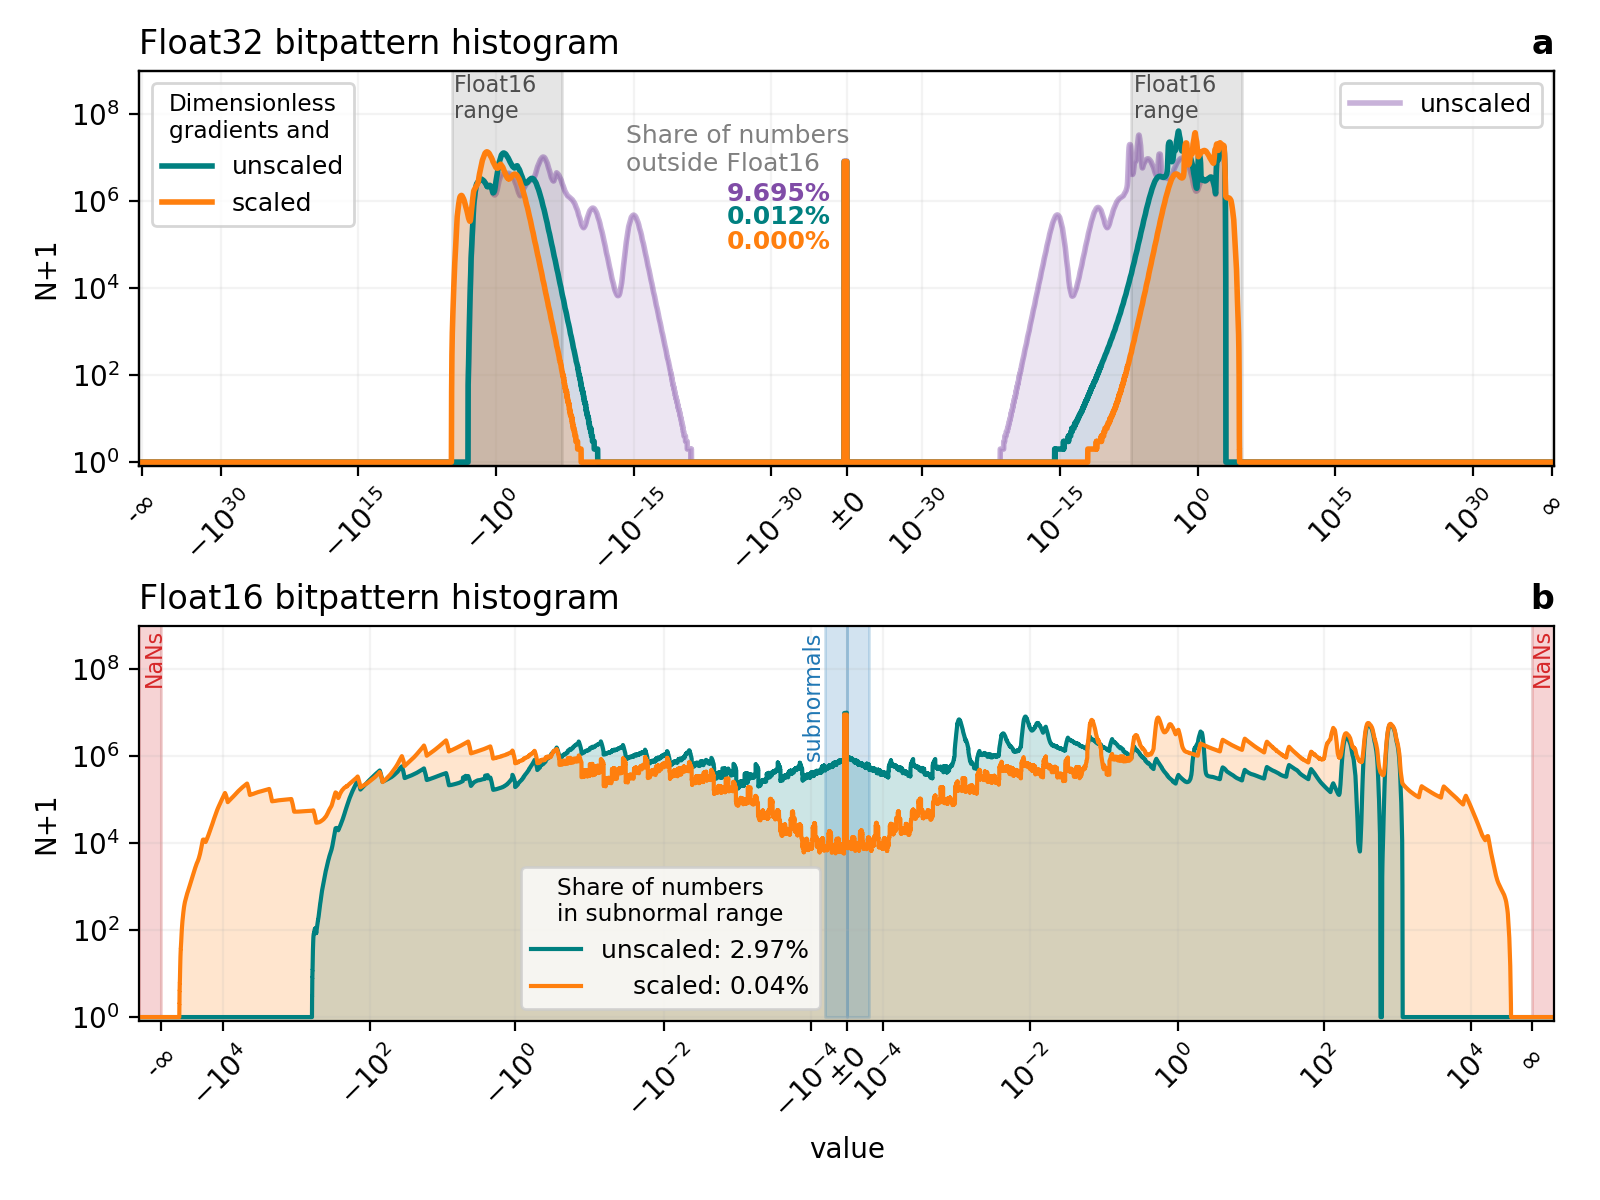
\includegraphics[width=1\textwidth]{Figures/a64fx/bitpattern_hist.png}
	\caption{\textbf{Bitpattern histogram of all arithmetic results in ShallowWaters.jl. a}
	200-day simulation at $\Delta x = 20\op{km}$ based on Float32 arithmetic. The share of numbers
	outside the Float16 range (grey shading) are colour-coded to the respective histograms. \textbf{b} as \textbf{a}
	but based on Float16. Bitpattern histograms are created with Sherlogs.jl. The logarithmic y-axis denotes the
	number of occurrences $N$ of the respective bitpattern during the simulation. The histograms span all
	available bitpatterns (\texttt{0x0000} to \texttt{0xffff} in hexadecimal) in the respective formats evenly
	but are sorted and relabelled with the corresponding values for readability. The range of bitpatterns that
	are subnormals or interpreted as Not-A-Number (NaN) are marked. Bitpatterns histograms are without
	compensated time integration.}
	\label{fig:a64fx_bitpatternhist}
\end{figure}

Using the DrWatson number format from Sherlogs.jl identifies the addition of the tendencies to the
prognostic variables $u,v,\eta$ as prone to produce subnormals (Listing \ref{lst:sherlogs}). We therefore
increase the scales  to scale up the prognostic variables and consequently their tendencies. Choosing
$s = 2^6, s_\eta = 1$ reduces the amount of subnormals to 0.04\%, while leaving about a factor two
headspace between the largest occurring numbers (about $30000$) to avoid overflows beyond $65504$
(Fig. \ref{fig:a64fx_bitpatternhist}b). The compensated time integration (see section
\ref{sec:compensated_time_integration}) increases this share to about 0.2\%.

The idealised tracer in ShallowWaters.jl takes values in (-1,1), so we scale this variable by $s_q = 2^{15}$
in order to use most of the Float16 range. This is to allow as many bitpatterns as possible for the interpolation
in the semi-Lagrangian advection scheme, which uses non-dimensional departure points on a locally relative
grid for 16-bit arithmetic, as described in section \ref{sec:swm_semilagrange}.

Consequently, the fully scaled shallow water equations are squeezed well into Float16, making near-optimal
use of the available bitpatterns, of which only 3\% are unused (NaNs excluded). In contrast, a simulation with
Float32 does not make use of at least 81\% of available bitpatterns (Fig. \ref{fig:a64fx_bitpatternhist}), assuming
that for a simulation run long enough all bitpatterns within the used range occur eventually. Extrapolating this
to Float64 with a representable range of $5 \cdot 10^{-324}$ to $2 \cdot 10^{308}$ the share of unused bitpatterns
is at least 97.5\%. This computational inefficiency can be overcome with 16-bit number formats and systematic
scaling as presented in this chapter. However, scaling leaves the precision issues with low-precision formats
unaddressed, for which we present the compensated time integration in the next section.

\subsection{A compensated time integration}
\label{sec:compensated_time_integration}

To minimise the precision loss in the time-integration, we adopt compensated summation as an alternative approach
to mixing precision. Compensated summation is a simple, yet powerful technique that prevents the accumulation of
rounding errors in the computation of large sums. Since the addition of multiple terms is ubiquitous in scientific computing,
compensated summation can be used to improve the accuracy of many algorithms such as numerical linear algebra
operations, integration or optimisation. Here we use compensated summation to augment the resilience to rounding
errors of our half-precision time-stepping method. 

The first version of compensated summation was used by \cite{Gill1951} in a Runge-Kutta integrator scheme in
fixed-point arithmetic, and the idea was subsequently extended to floating-point arithmetic by \cite{Kahan1965},
\cite{Moller1965} and others \citep{Vitasek1969,Linnainmaa1974,Higham1993}. That we are aware of, our paper
is the first work in which compensated summation is used in a fluid circulation model with 16-bit arithmetic.
To understand compensated summation, consider the following naïve algorithm for the summation of all the
entries of a length-$n$ vector $a$ with elements $a_i, i = 1,...,n$

\vspace{11pt}
\begin{lstlisting}[language=JuliaLocal,caption={\textbf{A naïve summation algorithm.}}]
sum = 0             # variable to store the sum
for ai in a         # loop over all elements of a
	sum += ai       # accumulate each element into sum   
end
return sum
\end{lstlisting}

This algorithm is prone to rounding errors, which accumulate at a rate proportional to $n$ \citep{Higham1993}.
Furthermore, the algorithm might cause stagnation, a phenomenon for which the partial sum becomes too large,
causing each subsequent addition to be neglected due to rounding. Compensated summation offers a much
better alternative at the cost of introducing an additional compensation variable \texttt{c} (Listing \ref{lst:compensated_summation})

\vspace{11pt}
\begin{lstlisting}[language=JuliaLocal,caption={\textbf{An algorithm for compensated summation.}},label=lst:compensated_summation]
c = 0                      # compensation, initially 0
sum = 0                    # variable to store the sum
for ai in a                # loop over all elements of a
	aic = ai - c           # compensate rounding error from previous iteration
 	temp = sum + aic       # add next element of a, but store in temp
	c = (temp-sum) - aic   # rounding error from sum+aic
 	sum = temp             # copy addition back to sum
end
return sum
\end{lstlisting}

At infinite precision, the compensation \texttt{c} will remain 0. At finite precision, however, calculating \texttt{c = (temp-sum) - aic}
will estimate the rounding error in the addition \texttt{sum + aic} and subsequently attempt to compensate for it in the next iteration
through \texttt{aic = ai - c}. For base-2 floating point arithmetic we have exactly \texttt{sum + ai = temp + c}, i.e. the compensation
variable \texttt{c} correctly captures the rounding errors in the addition. Compensated summation prevents the rounding errors
from accumulating, and the overall summation error will stay a mere multiple of machine precision \citep{Higham1993}. Overall,
the compensation \texttt{c} can be interpreted as a storage variable for rounding errors and effectively prevents rounding errors
in the summation from growing beyond machine precision.

Compensated summation is especially useful in settings in which the order of summation cannot be manipulated to prevent
rounding error growth. Time integration schemes, for which the state variables are updated sequentially, are especially
amenable to augmentation by compensated summation. Over a time period $T$ the number of terms to be added scales
as $T\Delta t^{-1}$, proportional to one for each time step. The naÏve algorithm would cause rounding errors to grow like
$\mathcal{O}(T\Delta t^{-1}\varepsilon)$, causing errors to counter-intuitively grow as the time-step is refined.
With compensated summation the rounding errors will stay $\mathcal{O}(\varepsilon)$.

ShallowWaters.jl uses the 4th-order Runge-Kutta scheme \citep{Butcher2008} to integrate the non-dissipative terms in time:
The momentum advection $\mathbf{u} \cdot \nabla \mathbf{u}$;
the Coriolis force $f\mathbf{\hat{z}} \times \mathbf{u}$;
the pressure gradient $-g\nabla \eta$;
the wind forcing $\mathbf{F}$;
and the conservation of volume $-\nabla \cdot (\mathbf{u} h)$ are summarised as the right-hand side function $\op{rhs}$.
The time integration is now augmented with compensated summation. The rounding error $c_u$ that occurs in the addition
of the total tendency $du$ to the previous time step $u_n$ is calculated and stored. On the next time step, this rounding error
is subtracted from the total tendency $du$ in an attempt to compensate for the rounding error from the previous time step.
This is illustrated here for the zonal velocity $u$ in isolation, although in practice the time integration has to update the
prognostic variables $u,v,\eta$ simultaneously. A compensated time integration for $u$ with RK4 can be written as
\begin{align}
k_1 &= \op{rhs}(u + \tfrac{\Delta t}{2}k_1), \nonumber \\
k_2 &= \op{rhs}(u + \tfrac{\Delta t}{2}k_2), \nonumber \\
k_3 &= \op{rhs}(u + \tfrac{\Delta t}{2}k_3), \nonumber \\
k_4 &= \op{rhs}(u + \Delta t k_3), \nonumber \\
du &= \tfrac{\Delta t}{6}(k_1 + 2k_2 + 2k_3 + k_4), \nonumber \\
u_{n+1}^* &= u_n + du, \nonumber \\
c_u &= (u^*_{n+1} - u_n) - du,
\label{eq:RK4_compensated}
\end{align}
with $c_u = 0$ as initial condition. The addition $u_n + du$ usually suffers from rounding errors as described above.
The loss of precision in $du$ is calculated in $c_u$ (which is only 0 in exact arithmetic). The compensation is analogously
implemented with $c_v,c_\eta$  for the other prognostic variables.  

The dissipative terms, i.e. biharmonic diffusion of momentum $\nu_B\nabla^4\mathbf{u}$ and bottom friction $-r\mathbf{u}$,
are integrated with a single forward step after the Runge-Kutta integration in ShallowWaters.jl and summarized as 
$\op{rhs}_{\op{diss}}$. To compensate for rounding errors for both the dissipative and non-dissipative terms simultaneously,
$c_u$ from Eq. \ref{eq:RK4_compensated} is subtracted from the total dissipative tendency $du_{\op{diss}}$.
In that sense, the rounding error from Eq. \ref{eq:RK4_compensated} is attempted to be compensated subsequently
in Eq. \ref{eq:RK4_compensated2}, and vice versa.
\begin{align}
du_{\op{diss}} &= \Delta t \op{rhs}_{\op{diss}}(u_{n+1}^*) - c_u, \nonumber \\
u_{n+1} &= u^*_{n+1} + du_{\op{diss}}, \nonumber \\
c_u &= (u_{n+1} - u_{n+1}^*) - du_{\op{diss}}.
\label{eq:RK4_compensated2}
\end{align}
Only the addition of the total tendency is compensated here to minimise the amount of additional calculations, which
increases when also compensating the 3 sub steps in RK4.

The compensated time integration is an alternative to mixed-precision approaches. While those aim to keep the precision
high in the precision-critical calculations, the compensated time integration introduces a new variable to compensate for
the rounding errors in one precision-critical calculation. With compensated time integration all variables can be kept in 16 bit,
and no conversions between number formats are necessary.

\begin{figure}[tbhp]
	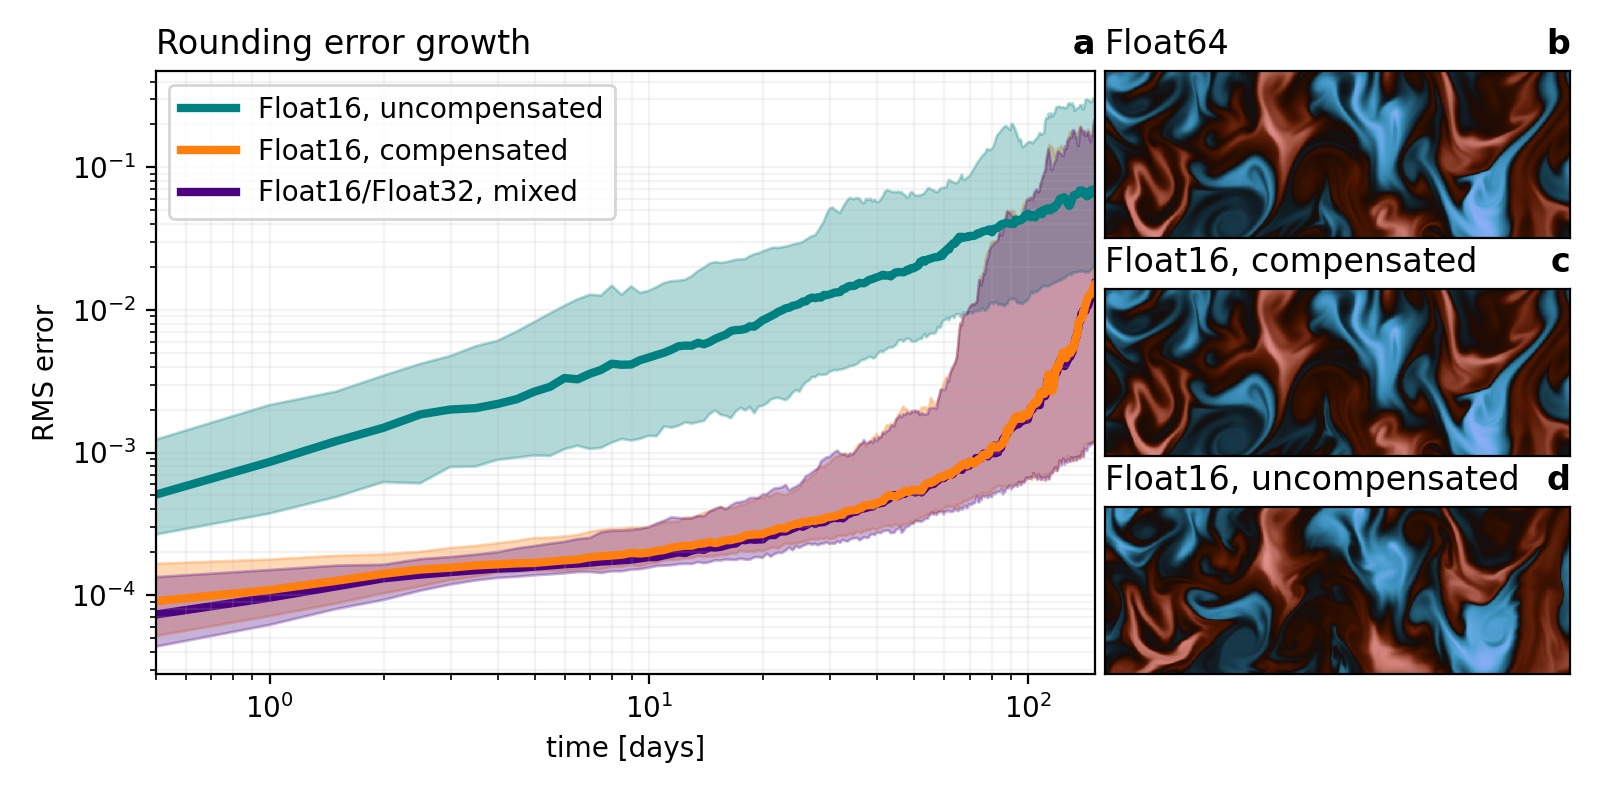
\includegraphics[width=1\textwidth]{Figures/a64fx/error_growth.png}
	\caption{\textbf{Rounding error growth with Float16 in ShallowWaters.jl
	using compensated time integration or mixed precision. a}
	Errors are root-mean square (RMS) errors of zonal velocity $u$ relative to Float64. Solid lines denote the median
	and shadings the interdecile confidence interval. \textbf{b,c} Snapshots of tracer $q$ from a zoom into
	Fig. \ref{fig:a64fx_tracermixing} after 100 days of simulation and \textbf{d} as \textbf{c} but without
	compensated time integration.}
	\label{fig:a64fx_error_growth}
\end{figure}

\section{Results}
\label{sec:hardware_speedup}

\subsection{Minimizing precision issues in 16 bit}
The accumulated rounding error from mixing precision and compensated time integration is now assessed.
ShallowWaters.jl is started from identical, in Float16 perfectly representable, initial conditions in a domain of
8000~km by 4000~km. The model is spun-up to reach a turbulent flow domain-wide, while the tracer starts from
an idealised checkerboard pattern to better highlight the turbulence everywhere in the domain.  The grid consists
of 3000x1500 points at about 2.7~km grid-spacing. With Float16 and without compensated time integration,
the accumulated rounding error for zonal velocity $u$ compared to Float64 exponentially increases 100-fold in
the first 150 days (Fig. \ref{fig:a64fx_error_growth}a). With mixed precision, using Float16 for the tendencies
and Float32 for the prognostic variables (see section \ref{sec:swm_results_mixed}), this rounding error growth
is strongly reduced. Errors after a few time steps without mixed precision are reached after about 100 days
(about 25,000 time steps) of integration. After that the error growth accelerates and chaos removes the
information of the initial conditions.

Using a compensated time integration, the rounding error from Float16 is strongly reduced and matches well with the
error growth of mixed precision. From the perspective of rounding errors the two methods are therefore equivalently
suited to reduce rounding errors with 16-bit arithmetic. The rounding error growth of the other prognostic variables is
similar. The positive effect of compensated time integration is well illustrated in snapshots of tracer mixing where even
after 100 days of simulation only a very slight deviation from the Float64 reference is observable
(Fig. \ref{fig:a64fx_error_growth}b, c and d).

\begin{figure}[tbhp]
	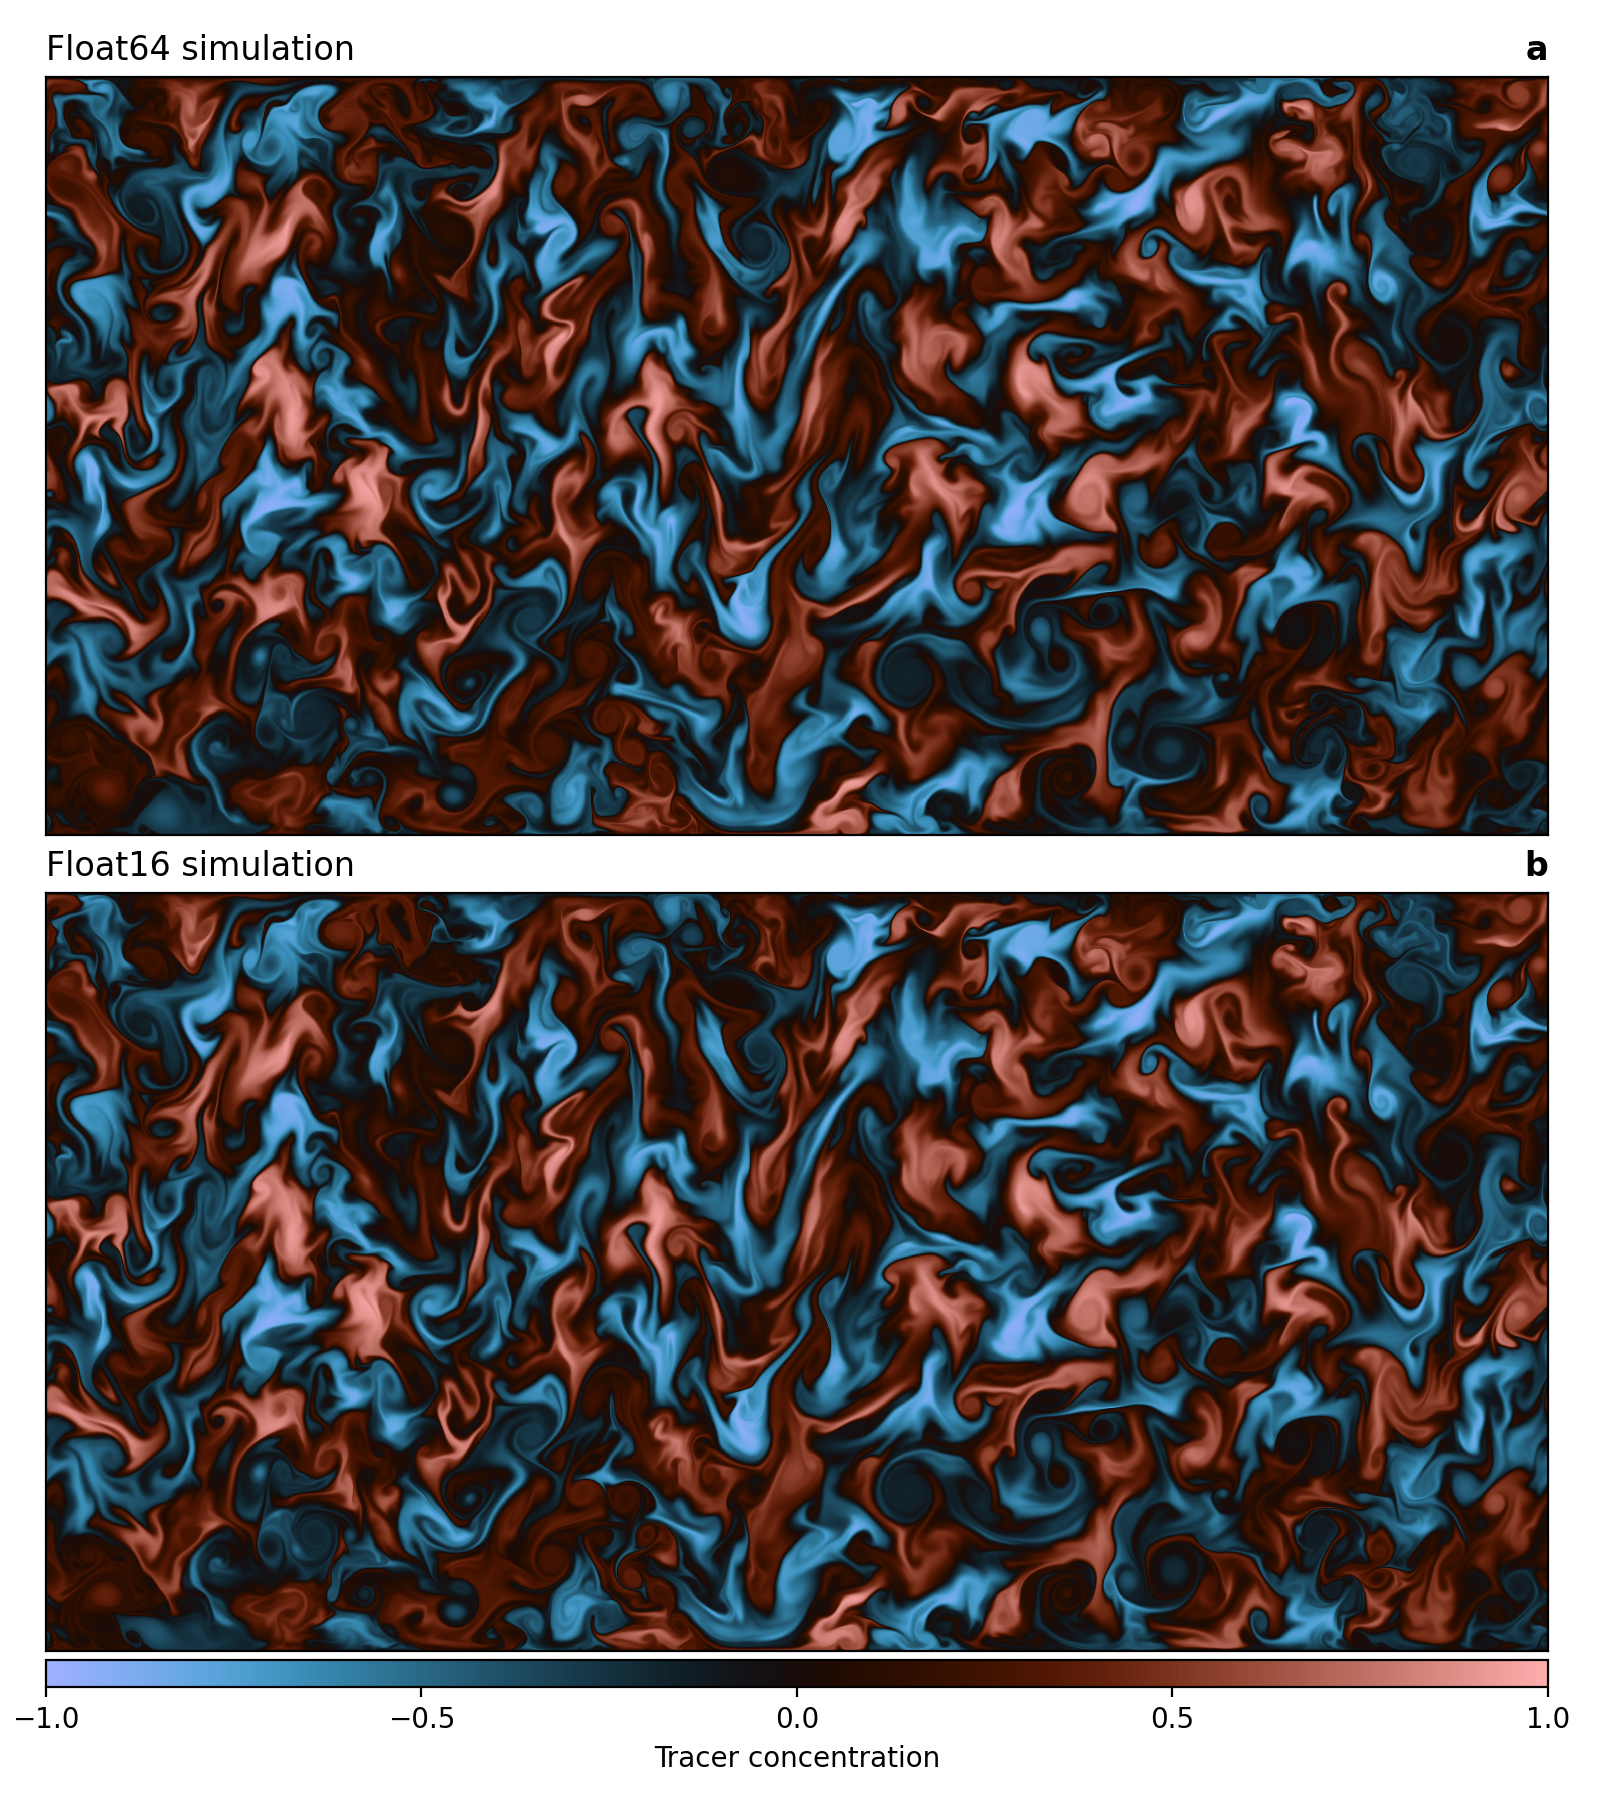
\includegraphics[width=1\textwidth]{Figures/a64fx/frame_hr_0199.png}
	\caption{\textbf{Turbulent tracer mixing as simulated by ShallowWaters.jl. a}
	Simulation based on Float64 arithmetic and \textbf{b} Float16 with compensated time integration.
	Snapshot is taken after 100 days of simulation (about 25,000 time steps) with 3000x1500 grid points
	starting from identical initial conditions. Remaining errors between \textbf{a} and \textbf{b} from
	low-precision Float16 are tolerable and will be masked by other sources of error in a less
	idealised model setup.}
	\label{fig:a64fx_tracermixing}
\end{figure}

Even after 100 days of simulation a large simulation (3000x1500 grid points) with Float16 shows minimal errors in
the tracer mixing compared to Float64 (Fig. \ref{fig:a64fx_tracermixing}). Only at regions near the boundaries,
where the mixing is enhanced, a difference is visible. The remaining rounding error is small and will be masked
in a more realistic setup by model or discretization errors. Reducing the precision in calculations raises concerns
about the numerical conservation of physically conserved quantities like mass. The compensated time integration
conserves the mass in the shallow water equations with Float16 (<0.002\% change within 500 days compared to Float64),
similar to mixed precision (Fig. \ref{fig:a64fx_conservation}). Without compensated time integration for Float16 the conservation is with
0.05\% change over 500 days less accurate. Similar results were obtained for the conservation of the tracer.
We will now assess the speedups with Float16 compared to Float64 on A64FX.

\begin{figure}[tbhp]
	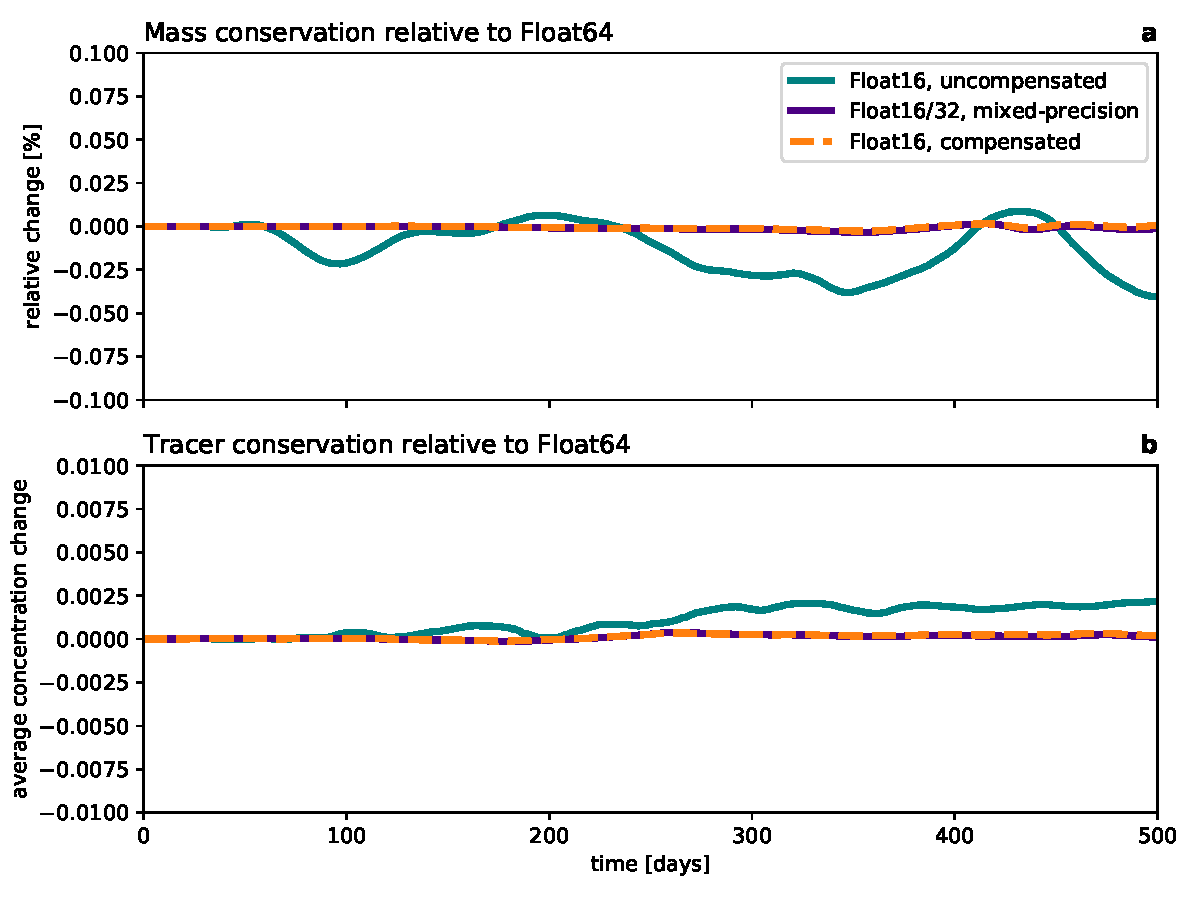
\includegraphics[width=1\textwidth]{Figures/a64fx/conservation.pdf}
	\caption{\textbf{Mass and tracer conservation with Float16 arithmetic. a}
	Mass conservation relative to Float64. \textbf{b} Tracer conservation relative to Float64 in units of tracer
	concentration with initial conditions in (-1,1), see Fig. \ref{fig:a64fx_tracermixing}. Both mass and tracer
	are well conserved with Float16 arithmetic. Best conservations are obtained with compensated time
	integration or mixed precision.}
	\label{fig:a64fx_conservation}
\end{figure}

\subsection{Approaching 4x speedup on A64FX}
The A64FX is a microprocessor developed by Fujitsu based on the ARM-architecture. It powers not just the fastest
supercomputer in the world as of June 2021 (measured by \href{https://top500.org}{TOP500}, \cite{Dongarra2011}),
Fugaku, but also a number of smaller systems around the world, including Isambard 2 which we use here. The A64FX
has a number of features intended to accelerate machine learning applications. Notably, it allows not just Float32 and
Float64 arithmetic but also Float16. Official benchmarks of the A64FX demonstrate a cost increase which is linear
with the number of bits. In that sense, Float32 can be twice as fast in applications than Float64, while Float16 can
be four times as fast, when optimized well. In practice, speedups in complex applications are due to a mix of factors:
In compute-bound applications, the wall-clock time is largely given by the clock rate of the processor and the
vectorization of arithmetic operations (such that small sets of them are performed in parallel on a single processor core).
Using Float16 instead of Float64 allows to put four times as many numbers through the vectorization, theoretically
allowing for 4x speedups. The performance of memory-bound applications, on the other hand, is largely determined
by the data transfer rate between the processor and its various levels of caches that increase in size but decrease
in bandwidth. Using Float16 instead of Float64 allows to load four times as many numbers from memory,
which theoretically translates to 4x speedup as well. 

\begin{figure}[tbhp]
	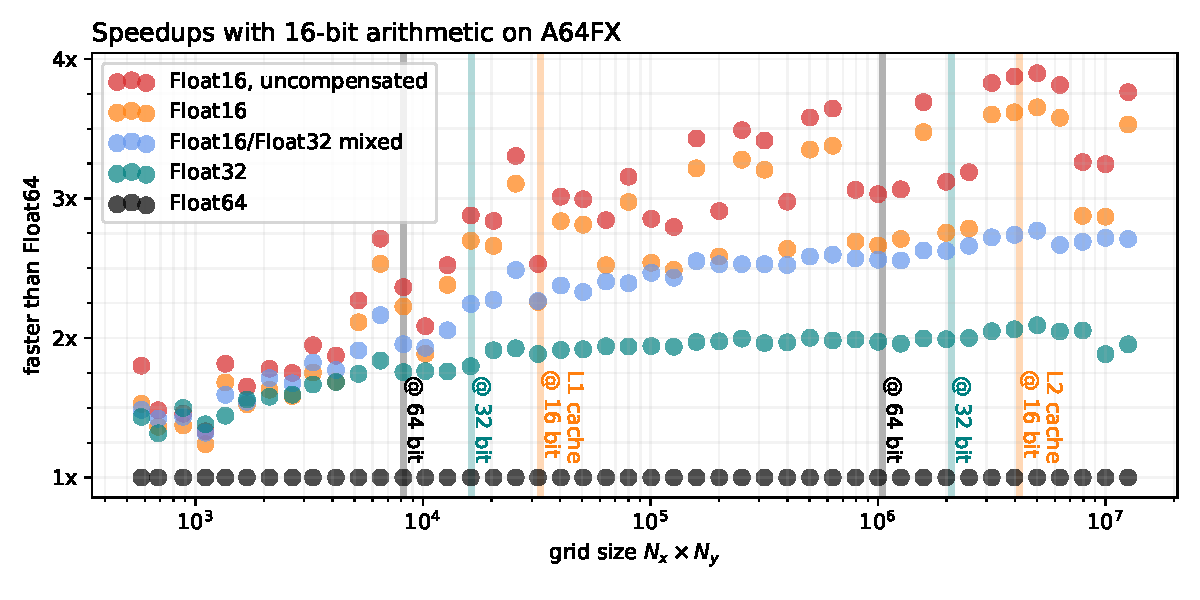
\includegraphics[width=1\textwidth]{Figures/a64fx/speedup.pdf}
	\caption{\textbf{Performance increase from Float16 when running ShallowWaters.jl at varying grid sizes
	on A64FX.} The grid size is the total number of grid points $N_x \times N_y$. All timings are single-threaded
	median wall clock times relative to Float64, excluding compilation, model initialisation and memory pre-allocation.
	The corresponding size of the L1 and L2 cache (64KiB, 8 MiB) of A64FX is given as vertical lines for arrays
	of 16, 32 and 64-bit floats.}
	\label{fig:a64fx_speedup}
\end{figure}

ShallowWaters.jl is a memory-bound application for which the biggest benefit from Float16 will be the reduction of
the size of the arrays by a factor of four when compared to Float64. The arrays can therefore be read faster from
memory with a potential speedup of 4x. We benchmark ShallowWaters.jl at varying grid sizes, excluding compilation,
model initialisation and memory pre-allocation. With grid sizes of $10^5$ (about 450x225 grid points) and larger,
there is a clear improvement from using Float32 instead of Float64 which approaches 2x speedups (Fig.
\ref{fig:a64fx_speedup}). Using Float16 these speedups reach up to 3.8x for grid sizes beyond $3 \cdot 10^6$
(about 2450x1225 grid points). The dependency of the speedup on the grid size is complicated:
While larger grids usually experience more acceleration on A64FX in Float16, there are ranges where the speedup
drops to 3-3.25x. This is likely due to peculiarities in the memory and cache hierarchy of the
A64FX, such that the performance benefit of Float16 cannot always be fully realised. A detailed assessment of these
peculiarities is beyond the scope of this chapter, but it is nevertheless reassuring that, even in the worst case, Float16
is still at least three times faster than Float64 for these large grids. 

As discussed in previous sections, using a compensated time integration can be used to minimise the rounding errors,
which comes with a small additional computational cost: Using the compensated time integration the speedups drop to
about 3.6x for large grids. Nevertheless, a compensated time integration yields higher performances than mixing the
precision of Float16 and Float32, which approaches only 2.75x here. Consequently, a compensated time integration
for Float16 is, although as precise, faster than mixed precision.

\section{Discussion}
\label{sec:hardware_discussion}

Low-precision calculations for weather and climate simulations are a potential that is not yet fully exploited.
While the first weather forecast models are moving towards Float32, 16-bit arithmetics will likely find increasing
support on future supercomputers. Before the prevalence of 64-bit computing started in the 1990s, fluid models
were written for available 16 or 32-bit hardware. Since then scientific computing has focused on 64-bit precision
as higher performance through higher clock rates was expected to increase continuously \citep{Moore1998}.
We present, to our knowledge, the first modern fluid simulation that runs entirely in hardware-accelerated 16 bits
with minimal rounding errors but at almost 4x the speed. The simulations were performed on A64FX, the microprocessor
that is used in Fugaku, the fastest supercomputer as of November 2020 (\href{https://top500.org}{TOP500}, \cite{Dongarra2011}).

The complex partial differential equations underlying weather and climate simulations are difficult to fit into the
limited range of Float16, but here we have presented a method to do this more systematically. We present 
Sherlogs.jl to analyse number formats. Sherlogs.jl allows to assess any changes to the scaling of the equations
to minimise underflows while making the most of the available representable numbers. In our case,
subnormal floating-point numbers had to be avoided and scaling of the equations dropped the amount of
subnormals occurring from 10 to below 0.2\%.

Using 16-bit floats will likely cause precision issues in fluid simulations. While mixed precision has been
used to minimise rounding errors in precision-critical calculations, we have presented here an approach
that compensates for rounding errors to allow for simulations entirely within 16-bit arithmetic.
The compensated time integration minimises rounding errors from this precision-critical part of a simulation
at a slightly higher cost. Benchmarking in comparison to mixed precision shows that the compensated
time integration is faster in ShallowWaters.jl while being as precise as mixed precision.

Alternatives to floats have been discussed for weather and climate simulations previously \citep{Klower2019a,Klower2020a}.
Although posit numbers \citep{Gustafson2017a} are more precise in these applications, the improvement from floats to
posits is smaller than using mixed precision and therefore also smaller than the compensated time integration.
In that sense, algorithms that are low precision-resilient are far more important than the actual choice of the
number format, especially given that only floats are widely hardware-supported.

The work in this chapter shows that a naive translation of the mathematical equations into code will likely fail with 16-bit arithmetic.
However, this does not mean that 16-bit arithmetic is unsuited for the numerical solution of complex partial differential
equations such as the shallow water equations. But it means that both precision and range issues have to be addressed
in the design of the algorithms used. A compensated time integration is a low precision-resilient algorithm,
and scaling is essential to fit the very limited range of Float16. 

While 16-bit hardware is largely designed for machine learning, its potential to increase computational efficiency
extends to weather and climate applications too. 16-bit calculations are indeed a competitive way to also accelerate
Earth-system simulations on available hardware.


\chapter{Conclusions}
\label{chap:conclusions}
\section{Summary}

Numerical models of weather and climate are high-performance applications for the world's largest supercomputers, producing very large amounts of data. 
While 32 and 64-bit floating-point numbers are the only widely available number formats for scientific computing, this thesis investigates the potential
for lower precision computations and data compression for weather and climate modelling. An information-preserving compression for climate data
is derived, presented and discussed that distinguishes between the real and false information in data.



Low-precision climate computing can accelerate simulations
such that freed resources can be reinvested into improving 


\section{Discussion}
% \chapter{Outlook}
\label{chap:outlook}

%\chapter{Thesis outline}
\label{chap:outline}



\backmatter % book mode only
\appendix
\chapter{Appendix}
\markboth{\sc{Appendix}}{\sc{Appendix}}
\renewcommand{\thechapter}{A}

\section{Open-source software developments}
\label{sec:open}

\subsection{SoftPosit.jl}

\begin{itemize}
    \setlength\itemsep{-5pt}
    \item Authors: M Kloewer, M Giordano, C Leong
    \item URL: github.com/milankl/SoftPosit.jl
    \item License: MIT
    \item Version: 0.3.0
\end{itemize}

SoftPosit.jl is a software emulator for posit arithmetic. The package exports the Posit8, Posit16, Posit32 number types among other non-standard types, as well as arithmetic operations, conversions and additional functionality. The package is a wrapper for the SoftPosit C-library written by C Leong.

\subsection{StochasticRounding.jl}

\begin{itemize}
    \setlength\itemsep{-5pt}
    \item Authors: M Kloewer
    \item URL: github.com/milankl/StochasticRounding.jl
    \item License: MIT
    \item Version: 0.1.0
\end{itemize}

StochasticRounding.jl is a software emulator for stochastic rounding in the Float32, Float16 and BFloat16 number formats. Both 16bit implementations rely on conversion to and from Float32 and stochastic rounding is only applied for arithmetic operations in the conversion back to 16bit. Float32 with stochastic rounding uses Float64 internally. Xoroshio128Plus is used as a high-performance random number generator.

\subsection{ShallowWaters.jl}

\begin{itemize}
    \setlength\itemsep{-5pt}
    \item Authors: M Kloewer
    \item URL: github.com/milankl/ShallowWaters.jl
    \item License: MIT
    \item Version: 0.3.0
\end{itemize}

ShallowWaters.jl is a shallow water model with a focus on type-flexibility and 16bit number formats, which allows for integration of the shallow water equations with arbitrary number formats as long as arithmetics and conversions are implemented. ShallowWaters also allows for mixed-precision and reduced precision communication.

ShallowWaters is fully-explicit with an energy and enstrophy conserving advection scheme and a Smagorinsky-like biharmonic diffusion operator. Tracer advection is implemented with a semi-Lagrangian advection scheme. Runge-Kutta 4th-order is used for pressure, advective and Coriolis terms and the continuity equation. Semi-implicit time stepping for diffusion and bottom friction. Boundary conditions are either periodic (only in x direction) or non-periodic super-slip, free-slip, partial-slip, or no-slip. Output via NetCDF.

\subsection{Sherlogs.jl}

\begin{itemize}
    \setlength\itemsep{-5pt}
    \item Authors: M Kloewer
    \item URL: github.com/milankl/Sherlogs.jl
    \item License: MIT
    \item Version: 0.1.0
\end{itemize}

Sherlogs.jl provides a number format Sherlog64 that behaves like Float64, but inspects your code by logging all arithmetic results into a 16bit bitpattern histogram during calculation. Sherlogs can be used to identify the largest or smallest number occuring in your functions, and where algorithmic bottlenecks are that limit the ability for your functions to run in low precision. A 32bit version is provided as Sherlog32, which behaves like Float32. A 16bit version is provided as Sherlog16{T}, which uses T for computations as well as for logging.

\subsection{Sonums.jl}

\begin{itemize}
    \setlength\itemsep{-5pt}
    \item Authors: M Kloewer
    \item URL: github.com/milankl/Sonums.jl
    \item License: MIT
    \item Version: 0.2.0
\end{itemize}

Sonums.jl is a software emulator for Sonums - the Self-Organizing NUMbers. A number format that learns from data. Sonum8 is the 8bit version, Sonum16 for 16bit computations.  The package exports number types, conversions and arithmetics. Sonums conversions are based on binary tree search, and arithmetics are based on table lookups. Training can be done via maximum entropy or minimising the rounding error.

\subsection{Float8s.jl}

\begin{itemize}
    \setlength\itemsep{-5pt}
    \item Authors: M Kloewer, J Sarnoff
    \item URL: github.com/milankl/Float8s.jl
    \item License: MIT
    \item Version: 0.1.0
\end{itemize}

Float8s.jl is a software emulator for a 8bit floating-point format, with 3 exponent and 4 significant bits. The package provides the \texttt{Float8} number type, as well as arithmetic operations, conversions and additional functionality. The software emulator is based on conversion to and from Float32, which is used for arithmetic operations.

\subsection{LogFixPoint16s.jl}

\begin{itemize}
    \setlength\itemsep{-5pt}
    \item Authors: M Kloewer
    \item URL: github.com/milankl/LogFixPoint16s.jl
    \item License: MIT
    \item Version: 0.1.0
\end{itemize}

LogFixPoint16s.jl is a software emulator for 16-bit logarithmic fixed-point numbers with 7 signed integer bits and 8 fraction bits. The package provides the \texttt{LogFixPoint16} number type, as well as arithmetic operations, conversions and additional functionality. The software emulator is based on either integer addition or look-up tables and is therefore a comparably fast emulator.

\subsection{Lorenz96.jl}

\begin{itemize}
    \setlength\itemsep{-5pt}
    \item Authors: M Kloewer
    \item URL: github.com/milankl/Lorenz96.jl
    \item License: MIT
    \item Version: 0.3.0
\end{itemize}

Lorenz96.jl is a type-flexible one-level Lorenz 1996 model, which supports any number type, as long as conversions to and from Float64 and arithmetics are defined. Different number types can be defined for prognostic variables and calculations on the right-hand side, with automatic conversion on every time step. The equations are scaled such that the dynamic range of numbers can be changed. The scaled equations are written division-free.

\subsection{Lorenz63.jl}

\begin{itemize}
    \setlength\itemsep{-5pt}
    \item Authors: M Kloewer
    \item URL: github.com/milankl/Lorenz63.jl
    \item License: MIT
    \item Version: 0.2.0
\end{itemize}

Lorenz63.jl is a type-flexible Lorenz 1963 model, which supports any number type, as long as conversions to and from Float64 and arithmetics are defined. The Lorenz equations are scaled such that the dynamic range of numbers can be changed. The scaled equations are written division-free.

\subsection{Jenks.jl}

\begin{itemize}
    \setlength\itemsep{-5pt}
    \item Authors: M Kloewer
    \item URL: github.com/milankl/Jenks.jl
    \item License: MIT
    \item Version: 0.1.0
\end{itemize}

Jenks.jl is the Jenks Natural Breaks Optimization, a data clustering method to minimise in-class variance or L1 rounding error. Jenks provides a data classification algorithm that groups one dimensional data to minimize an in-class error norm from the class mean but maximizes the same error norm between different classes.

%\chapter{Appendix B}
\ifpdf
    \graphicspath{{Appendix2/Appendix2Figs/PNG/}{Appendix2/Appendix2Figs/PDF/}{Appendix2/Appendix2Figs/}}
\else
    \graphicspath{{Appendix2/Appendix2Figs/EPS/}{Appendix2/Appendix2Figs/}}
\fi

\markboth{Appendix B}{Appendix B}

\section{Derivations}

%\bibliographystyle{plainnat}
%\bibliographystyle{Classes/CUEDbiblio}
\bibliographystyle{Classes/jmb} % bibliography style

\addcontentsline{toc}{chapter}{Acknowledgements}
\begin{acknowledgements}

I am very grateful for the support and very fruitful discussions with my supervisors Tim Palmer and Peter D\"{u}ben, and especially for the freedom to develop my own ideas.

 I would like to thank the whole Julia community for an uncountable effort to develop a very modern high performance computing language that is high-level, easy to learn and was proven to be increadibly useful for reduced precision simulations. I also would like to thank everybody who developed the matplotlib plotting library, which was used for every figure in this report.
 
\end{acknowledgements}


\addcontentsline{toc}{chapter}{Funding}
\begin{funding}

I gratefully acknowledge funding from
 
\begin{itemize}
\item[$\triangleright$] The European Research Council ERC under grant number 741112 \emph{An Information Theoretic Approach to Improving the Reliability of Weather and Climate Simulations}
\item[$\triangleright$] The UK Natural Environmental Research Council NERC under grant number NE/L002612/1.
\item[$\triangleright$] The Copernicus Programme (EU Commission) through the ECMWF Summer of Weather Code 2020 and 2021
\item[$\triangleright$] The Graduate Research Allowance provided by Jesus College Oxford in 2018 and 2019
\end{itemize}

\end{funding}


\newtotcounter{citnum}
\def\oldbibitem{} \let\oldbibitem=\bibitem
\def\bibitem{\stepcounter{citnum}\oldbibitem}

\renewcommand{\bibname}{References} % changes default name Bibliography to References
\bibliography{References/bibliography} % References file

\vspace{10pt}
\noindent \total{citnum} references in total.
\end{document}
